% Copyright (C) 2014-2016 by Thomas Auzinger <thomas@auzinger.name>

\documentclass[draft,final]{vutinfth} % Remove option 'final' to obtain debug information.

% Load packages to allow in- and output of non-ASCII characters.
\usepackage{lmodern}        % Use an extension of the original Computer Modern font to minimize the use of bitmapped letters.
\usepackage[T1]{fontenc}    % Determines font encoding of the output. Font packages have to be included before this line.
\usepackage[utf8]{inputenc} % Determines encoding of the input. All input files have to use UTF8 encoding.

% Extended LaTeX functionality is enables by including packages with \usepackage{...}.
\usepackage{amsmath}    % Extended typesetting of mathematical expression.
\usepackage{amssymb}    % Provides a multitude of mathematical symbols.
\usepackage{mathtools}  % Further extensions of mathematical typesetting.
\usepackage{microtype}  % Small-scale typographic enhancements.
\usepackage[inline]{enumitem} % User control over the layout of lists (itemize, enumerate, description).
\usepackage{multirow}   % Allows table elements to span several rows.
\usepackage{booktabs}   % Improves the typesettings of tables.
\usepackage{subcaption} % Allows the use of subfigures and enables their referencing.
\usepackage[ruled,linesnumbered,algochapter]{algorithm2e} % Enables the writing of pseudo code.
\usepackage[usenames,dvipsnames,table]{xcolor} % Allows the definition and use of colors. This package has to be included before tikz.
\usepackage{nag}       % Issues warnings when best practices in writing LaTeX documents are violated.
\usepackage{todonotes} % Provides tooltip-like todo notes.
\usepackage{rotating}  % Support for sideways figures
\usepackage{hyperref}  % Enables cross linking in the electronic document version. This package has to be included second to last.
\usepackage[acronym,toc]{glossaries} % Enables the generation of glossaries and lists fo acronyms. This package has to be included last.

% Define convenience functions to use the author name and the thesis title in the PDF document properties.
\newcommand{\authorname}{Robert Thurnher} % The author name without titles.
\newcommand{\thesistitle}{TempMunger} % The title of the thesis. The English version should be used, if it exists.

\DeclareMathOperator*{\argmin}{arg\,min}

% Set PDF document properties
\hypersetup{
    pdfpagelayout   = TwoPageRight,           % How the document is shown in PDF viewers (optional).
    linkbordercolor = {Melon},                % The color of the borders of boxes around crosslinks (optional).
    pdfauthor       = {\authorname},          % The author's name in the document properties (optional).
    pdftitle        = {\thesistitle},         % The document's title in the document properties (optional).
    pdfsubject      = {TempMunger},              % The document's subject in the document properties (optional).
    pdfkeywords     = {data wrangling, visual analytics, visual data transformation} % The document's keywords in the document properties (optional).
}

\setpnumwidth{2.5em}        % Avoid overfull hboxes in the table of contents (see memoir manual).
\setsecnumdepth{subsection} % Enumerate subsections.

\nonzeroparskip             % Create space between paragraphs (optional).
\setlength{\parindent}{0pt} % Remove paragraph identation (optional).

\makeindex      % Use an optional index.
\makeglossaries % Use an optional glossary.
%\glstocfalse   % Remove the glossaries from the table of contents.

% Set persons with 4 arguments:
%  {title before name}{name}{title after name}{gender}
%  where both titles are optional (i.e. can be given as empty brackets {}).
\setauthor{}{\authorname}{Bakk.}{male}
\setadvisor{Univ.Prof. Dr.}{Silvia Miksch}{}{female}

% For bachelor and master theses:
\setfirstassistant{Dr.}{Theresia Gschwandtner}{}{female}
%\setsecondassistant{Pretitle}{Forename Surname}{Posttitle}{male}
%\setthirdassistant{Pretitle}{Forename Surname}{Posttitle}{male}

% For dissertations:
%\setfirstreviewer{Pretitle}{Forename Surname}{Posttitle}{male}
%\setsecondreviewer{Pretitle}{Forename Surname}{Posttitle}{male}

% For dissertations at the PhD School and optionally for dissertations:
%\setsecondadvisor{Pretitle}{Forename Surname}{Posttitle}{male} % Comment to remove.

% Required data.
\setaddress{Neubaugasse 64-66, A-1070 Wien; \textcolor{blue}{\href{mailto:robert@thurnher.email}{robert[at]thurnher.email}}}
\setregnumber{0004297}
\setdate{13}{04}{2017} % Set date with 3 arguments: {day}{month}{year}.
\settitle{\thesistitle}{TempMunger} % Sets English and German version of the title (both can be English or German).
\setsubtitle{A Visual Analytics Approach Supporting Transformations of Time-Oriented Data}{Ein Visual Analytics Ansatz zur Transformation Zeitorientierter Daten} % Sets English and German version of the subtitle (both can be English or German).

% Select the thesis type: bachelor / master / doctor / phd-school.
% Bachelor:
%\setthesis{bachelor}
%
% Master:
\setthesis{master}
\setmasterdegree{dipl.} % dipl. / rer.nat. / rer.soc.oec. / master
%
% Doctor:
%\setthesis{doctor}
%\setdoctordegree{rer.soc.oec.}% rer.nat. / techn. / rer.soc.oec.
%
% Doctor at the PhD School
%\setthesis{phd-school} % Deactivate non-English title pages (see below)

% For bachelor and master:
\setcurriculum{Information \& Knowledge Management}{Information \& Knowledge Management} % Sets the English and German name of the curriculum.

% For dissertations at the PhD School:
%\setfirstreviewerdata{Affiliation, Country}
%\setsecondreviewerdata{Affiliation, Country}


\begin{document}

\frontmatter % Switches to roman numbering.
% The structure of the thesis has to conform to
%  http://www.informatik.tuwien.ac.at/dekanat

\addtitlepage{naustrian} % German title page (not for dissertations at the PhD School).
\addtitlepage{english} % English title page.
\addstatementpage

%\begin{danksagung*}
%\todo{Ihr Text hier.}
%\end{danksagung*}

\newcommand{\heart}{\ensuremath\heartsuit}

\begin{acknowledgements*}
Dedicated to my \textbf{father}\footnote{\emph{\textbf{RIP.}}}, my \textbf{mother}, and my \textbf{wife}. \\
This wouldn't have been possible if it weren't for you. \\
May it also motivate my \textbf{sister} pursuing her dreams. \\
\heart \\

I'd like to thank \emph{Theresia Gschwandtner} for her supervision, understanding, and patience.

Further thanks go out to my \textbf{brother} and \emph{Michael Jakl} for their support and inspiration.

Generally, I'm grateful to everyone who has test-driven the prototype, proofread drafts, and/or provided feedback -- particularly, my \textbf{sister-in-law} and \emph{CVAST} research staff.

\textbf{Thank you!}
\end{acknowledgements*}

\begin{kurzfassung}
\emph{Data-Wrangling} ist im Allgemeinen die mühevolle Aufbereitung von Daten um diese für nachfolgende Analysen nutzbar zu machen.
Normalerweise bedeutet das handgefertigte Skripte anzuwenden, was einen gewissen Grad an technischer Expertise verlangt.
Um derartiges Aufbereiten von Daten auch für User, die eher einer ``Casual''-Kategorie zuordenbar sind, zugänglich zu machen haben wir zur Erleichterung damit verbundener Aufgaben, im Kontext dieser Arbeit einen \emph{Visual-Analytics}-Prototypen erstellt.

Unser Ansatz ist ein interdisziplinärer, der zeitgemäße Konzepte und Ideen aus diversen Gebieten kombiniert:
\emph{Mensch-Computer-Interaktion} und \emph{Usability-Engineering} mit \emph{Information-Retrieval}, \emph{Data-Mining}, \emph{Machine-Learning} sowie \emph{Informationsvisualisierung}.

In diesem Zusammenhang konzentrieren wir uns speziell auf oftmals nötige Transformationsschritte von zeitorientierten Daten.
Diese Art von Daten weist einzigartige Charakteristika auf, die bei verschiedenen Lösungsansätzen gesondert berücksichtigt werden müssen.
Basierend auf den Ergebnissen einer Analyse des State-of-the-Art in diesem Bereich, haben wir offene Fragestellungen sowie einige Anforderungen für einen solchen Prototypen abgeleitet und folglich einen Software-Prototyp namens \textbf{\emph{TempMunger}} in einer agilen Art und Weise iterativ sowohl designt als auch entwickelt.
Der Prozess sowie dazugehörige Artefakte werden umfassend dokumentiert und dargestellt.

Unser Prototyp ist eine web-basierte Anwendung, die für den Gebrauch mittels Desktop-Browser zugeschnitten ist.
Genauer gesagt, bietet sie interaktive Dashboard-Visualisierung-en für möglichst intuitive sowie explorative Transformationsoperationen zeitorientierter Daten.
Eine qualitative Evaluierung des Prototypen zeigte, dass diese Funktionalität als nützlich empfunden wird.
Außerdem ergaben sich verschiedene Ideen für künftige, weiterführende Arbeiten.

Abschließend kann man sagen, dass Data-Wrangling ein spannendes Forschungsgebiet bleibt, in dem es noch viel zu entdecken gilt.
\end{kurzfassung}

\begin{abstract}
\emph{Data wrangling} generally denotes the cumbersome task of making data useful for analysis.
Usually, this means applying hand-crafted scripts, requiring at least a certain degree of technical expertise.
In order to make suchlike data preparation accessible for rather casual users as well, we have built a \emph{visual analytics} prototype in the context of this thesis, easing related tasks.

Our approach is an interdisciplinary one, combining contemporary concepts and ideas from various fields:
\emph{human-computer interaction} and \emph{usability engineering} with \emph{information retrieval}, \emph{data mining}, \emph{machine learning}, plus \emph{information visualization}.

In particular we focus on supporting transformations of time-oriented data since this kind of data exhibits unique characteristics which demand for special consideration.
After analyzing related state of the art we identified open issues and derived requirements for such a system. We followed an iterative design process to develop a software prototype called \textbf{\emph{TempMunger}}, in an agile manner.
The process as well as corresponding artifacts are documented and presented in this thesis.

Our prototype is a web-based application, tailored for desktop browser usage.
More concretely, it offers interactive dashboard visualizations for preferably intuitive and exploratory transformation operations of time-oriented data.
A qualitative evaluation of the prototype demonstrates its usefulness and reveals opportunities for future work.

Concluding it is safe to say that data wrangling continues to be an exciting field of research where much is yet to be discovered.
\end{abstract}

% Select the language of the thesis, e.g., english or naustrian.
\selectlanguage{english}

% Add a table of contents (toc).
\tableofcontents % Starred version, i.e., \tableofcontents*, removes the self-entry.

% Switch to arabic numbering and start the enumeration of chapters in the table of content.
\mainmatter

%%%%%%%%%%%%%%%%%%%%%%%%%%%%%%%%%%%%%%%%%
\chapter{Introduction}
\label{ch:intro}
%%%%%%%%%%%%%%%%%%%%%%%%%%%%%%%%%%%%%%%%%

\newacronym{va}{VA}{Visual Analytics}
\newacronym{ml}{ML}{Machine Learning}
\newacronym{hci}{HCI}{Human-Computer Interaction}
\newacronym{ux}{UX}{User Experience}
\newacronym{ui}{UI}{User Interface}
\newacronym{ir}{IR}{Information Retrieval}
\newacronym{infovis}{InfoVis}{Information Visualization}
\newacronym{cvast}{CVAST}{Centre for Visual Analytics Science and Technology}

\newglossaryentry{datascience}
{
  name={data science},
  description={concerns itself with gaining insights from data scientifically}
}
\newglossaryentry{datawrangling}
{
  name={data wrangling},
  description={consists of techniques being applied to transform data}
}
\newglossaryentry{datamunging}
{
  name={data munging},
  description={is a synonym for \gls{datawrangling}}
}
\newglossaryentry{datamining}
{
  name={data mining},
  description={consists of techniques being applied, mainly , for \gls{ml}}
}


\section{Motivation}

Applied work within \gls{datascience}, and more specifically \textbf{\gls{va}}, \emph{``the science of
analytical reasoning facilitated by interactive visual interfaces''}~\cite{Thomas2005} (p. 4), can be seen to roughly consist of three main basic building blocks~\cite{Web:DataScience}:
\begin{enumerate}
  \item \textbf{\Gls{datawrangling}} a.k.a. \textbf{\glslink{datamunging}{munging}}
  \item Statistics\index{statistics} \& \Gls{ml}
  \item Visualization \& analysis\index{analysis} itself
\end{enumerate}

While the second and last mentioned fields are constantly evolving related tools and techniques, the first one is comparatively still lacking in terms of high-level support.
This is when it comes down to actually wrangle\index{wrangle} usually messy real-world data into a format prepping it useful for analysis\index{analysis}.

To this day, it mostly means fiddling around with the data manually, applying hand-crafted transformation\index{transformation} scripts.
This is a tedious task and discourages analyzing data altogether, especially if the ones intending to work with the data are technically unversed (for instance, journalists or business analysts).

However, combining contemporary knowledge and technology from the domains of \emph{\gls{hci}}~\cite{Cooper2004} \& \emph{\gls{ux}}~\cite{Norman2002} as well as \emph{\gls{ir}}~\cite{Manning2008}, \emph{\gls{datamining}} / \emph{\Gls{ml}}~\cite{Witten2011}, and \emph{\gls{infovis}}~\cite{Tufte2001}~\cite{Card1999}, could yield substantial improvements here.

Namely, making \gls{datawrangling} accessible to a wider audience, mainly by providing interactive analytical visualizations allowing for easy data transformations\index{transformation} and giving immediate visual feedback.

In this thesis we are investigating the field of \gls{datawrangling}, plus, designing\index{design}, and prototypically\index{prototype} implementing a \gls{va} approach\index{approach} to support the tasks involved.
That is, iteratively creating a software prototype\index{prototype} which enables users to wrangle\index{wrangle} data suitable for analysis\index{analysis} in an intuitive, interactive, and visual way.

\Gls{va} and \gls{infovis} enable uncovering the non-obvious by using interactive visualizations.
Consequently, this approach is especially useful when applied to complex tasks where clear overview and structuring is necessary in order to achieve effective results efficiently.
That is also why employing related techniques can generally be expected to be more successful for the outlined use case than fully automated ones.
Hence, an ideal solution would probably be a blend of automated suggestions, augmenting an interactive interface driven by visualizations.

Additionally, the to-be-developed prototype\index{prototype} shall, in particular, make it convenient to work on time-oriented\index{time-oriented} datasets. Time itself and time-oriented\index{time-oriented} data, specifically, possess distinct characteristics (for instance, regarding scale, scope, structure, viewpoint, and granularity) that make it worthwhile to dedicatedly treat it as a separate data type, as suggested by Aigner et al.~\cite{Aigner2011}.
This is why time-oriented\index{time-oriented} data demands for special \gls{datawrangling} solutions which have not been adequately tackled yet.


\section{Problem Statement}

The main research question in the context of this work is:

\textbf{\emph{How can we support \gls{datawrangling} with \gls{va} techniques?}}
\\\\
More particular, we are to tackle the following subquestions:

\begin{itemize}
  \item \emph{Which data transformations\index{transformation} are best supported by analytical methods and for which transformations\index{transformation} is visual support beneficial?}
  \item \emph{How do concrete \gls{datawrangling} workflow processes look like and how can these processes be supported by \gls{va} methods?}
  \item \emph{What \gls{datawrangling} tasks need to be tackled in particular when dealing with time-oriented\index{time-oriented} data and how can we support them with \gls{va} methods?}
\end{itemize}

The emphasis of this thesis is put on evaluating the feasibility of corresponding concepts via iterative design\index{design}, implementation, and evaluation of a software prototype\index{prototype}.


\section{Aim of the Work}

Results to be achieved are:

\begin{itemize}
  \item Design\index{design} and implementation of a research prototype\index{prototype}
  \item Evaluation of the prototype to answer research questions
  \item Detailed documentation of these
\end{itemize}

At the end of the project, it should be known whether developing such a \textbf{prototype}\index{prototype} supporting these tasks is feasible and if so, how in detail.
As mentioned above, the approach\index{approach} shall combine concepts from \gls{hci} \& \gls{ux} with ones from \gls{ir}, \gls{ml}, and \gls{va}.
Special focus will be laid on crafting the \textbf{\gls{ui}} and an underlying \textbf{analytical inference engine}, interactively providing the user with respective data quality and potential issue suggestions visually. Furthermore, \textbf{direct manipulation} of data should be easy.
Plus, transformations\index{transformation} shall, generally, be easily applicable to \textbf{batches of data} by making use of bulk operations, while again being visual-interactively supported.
A central challenge is making this all work in the context of \textbf{time-oriented\index{time-oriented} data}.

Answers to the stated research questions are intended to be given by designing\index{design}, implementing, and evaluating a research prototype\index{prototype} which provides \gls{va} techniques to improve and support \gls{datawrangling} tasks.


\section{Methodological Approach}

In order to answer our research questions we follow the nested model by Munzner~\cite{Munzner2009}. In particular we include the following steps:

\begin{enumerate}
  \item \textbf{State of the art review}: giving an overview of the topic, spanning from scientific foundation to various approaches\index{approach}, and serving as first input to our approach\index{approach}.
  \item \textbf{Requirements analysis\index{analysis}}: determining which features to implement, directed to answering why, what, and how.
  \item \textbf{Design\index{design} of interactive visualizations}: subsequent iterative design\index{design} process, making use of state-of-the-art tools.
  \item \textbf{Iterative prototypical\index{prototype} implementation}: following an agile approach\index{approach} until satisfying results are achieved.
  \item \textbf{Qualitative evaluation of results}: for validating fulfillment of goals and, consequently, leading to answering our research questions.
\end{enumerate}

In the context of this work, we also consider the \emph{data--users--tasks} triangle for \gls{va}.
This triangle can be seen in Figure~\ref{fig:cvast-triangle} and is introduced in \cite{Miksch2014}.
It is particularly useful for initial requirements analysis\index{analysis} of a visualization project.
Consequently, we apply it as a starting point.
Its basic notion is to think of a product for \gls{va} within the three dimensions of data, users, and tasks separately, first, and then in interplay.
The latter, thus, defines effectiveness, expressiveness, and appropriateness of the to-be-chosen interactive \gls{va} methods, as visualized in the diagram.

\begin{figure}[h]
  \centering
  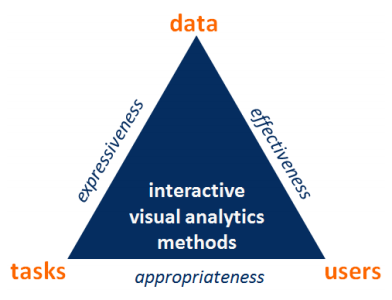
\includegraphics[width=0.725\textwidth]{figures/introduction/cvast-triangle}
  \caption{The \emph{data--users--tasks} triangle as presented in \cite{Miksch2014}.}
  \label{fig:cvast-triangle}
\end{figure}

All steps are accurately documented, emphasizing findings of the evaluation and lessons learned.
The thesis covers all aspects and results of the design\index{design}, development, and evaluation of the prototype\index{prototype}, from mockups and architectural\index{architecture} diagrams to test results.


\section{Structure of the Work}

The thesis is structured as follows:

\begin{enumerate}
  \item An \textbf{introduction} to the topic and thesis itself: this presents the motivation, problem statement, and methodological approach\index{approach}.
  \item A \textbf{state of the art} review: this is laying out the scientific foundation regarding our topic and showing various approaches\index{approach}. The latter are, thus, analyzed and compared. It is closed by a crossover to the requirements analysis\index{analysis} for our approach\index{approach}, fueled with preceding input.
  \item A \textbf{design\index{design} and implementation} chapter: this is describing, explaining, and documenting all connected steps thoroughly. The design\index{design} section consists of creating personas, wireframing with mockups, and consequently deriving our requirements. The implementation section walks through the developed prototype\index{prototype}, looking at it from varied angles, and presents its qualitative evaluation.
  \item A concluding section with \textbf{critical reflection} of the achieved work: this includes comparing with related work, discussing open issues, and answering our research questions. It is also concerning the requirements we have previously derived.
  \item Finally, closing the thesis with a \textbf{summary and future work} section: this is just briefly summing up our work and offering an outlook.
  \item At the end, there is an \textbf{appendix}: this contains a detailed presentation of the software design\index{design} and architecture\index{architecture} of our prototype\index{prototype} as well as scientific background, plus further implementation details.
\end{enumerate}



%%%%%%%%%%%%%%%%%%%%%%%%%%%%%%%%%%%%%%%%%
\chapter{State of the Art}
\label{ch:state-of-the-art}
%%%%%%%%%%%%%%%%%%%%%%%%%%%%%%%%%%%%%%%%%

\newacronym{rnd}{R\&D}{Research and Development}
\newacronym{etl}{ETL}{Extract, Transform, Load}
\newacronym{rdbms}{RDBMS}{Relational Database Management System}
\newacronym{pbe}{PBE}{Programming by Example}
\newacronym{lpbd}{L/PBD}{Learning/Programming by Demonstration}
\newacronym{gui}{GUI}{Graphical User Interface}
\newacronym{dsl}{DSL}{Domain-Specific Language}
\newacronym{ide}{IDE}{Integrated Development Environment}
\newacronym{rdf}{RDF}{Resource Description Framework}
\newacronym{rcp}{RCP}{Rich Client Platform}
\newacronym{cli}{CLI}{Command Line Interface}
\newacronym{repl}{REPL}{Read--Eval--Print Loop}

\newglossaryentry{datawarehousing}
{
  name={data warehousing},
  description={is a classic approach to analytical reporting based on data marts mostly periodically fed from multiple sources}
}

\newglossaryentry{semanticweb}
{
  name={semantic web},
  description={is a buzzword term commonly subsuming approaches and technologies supporting the notion of making the mainly text-based, unstructured data on the \textsc{WWW} more accessible by enriching it with machine-readable semantics}
}


The report or review contained in this chapter focuses on summarizing and comparing approaches\index{approach}, techniques, and related work within the field which can generally be subsumed by the term \emph{``\textbf{\gls{datawrangling}}''} with an emphasis on \textbf{visual-interactive\index{visual-interactive} support}.
This is a relatively young field of interdisciplinary \gls{rnd}.
It is basically about the process of making any data useful for analysis\index{analysis}.
This reviewing report is mainly geared towards offering an overview of the topic in order to comprehensively show differences of existing approaches\index{approach} as well as commonalities shared between them.
Furthermore, special attention is paid to setting it all into the historic evolutionary context of the field.
In the end, we can see that there is still some need for exploration and improvements here, particularly regarding visual-interactive\index{visual-interactive} components and the support for time-oriented\index{time-oriented} data.

This chapter gives a brief overview of related work, i.e., its scientific underpinnings, followed by a walkthrough of different concrete approaches\index{approach}, techniques, and related tools.

\section{Literature Study}

Generally, \cite{Kandel2011a} was used as a point of origin to find other relevant references.
Then, going through the list of references of these papers, relevance was determined via personal evaluation.
Plus, we scanned the reference lists of thus relevant papers.

Moreover, we searched the archives of topic-related journals (i.e., \emph{Information Visualization Journal} and \emph{ACM Journal of Data and Information Quality}) as well as scientific, electronic databases (\emph{ACM Digital Library}, \emph{IEEE Xplore}, and also \emph{Google Scholar}) and proceedings of relevant conferences (\emph{International Conference on Information Visualization}, \emph{IEEE Conference on Visual Analytics}, \emph{ACM SIGCHI Conference on Human Factors in Computing Systems}, etc.).

Our search terms included \emph{``data wrangling''}, \emph{``data cleansing''}, and variations of these phrases.
\emph{Mendeley}\footnote{\textcolor{blue}{\href{https://www.mendeley.com/}{www.mendeley.com}}} was used as a tool to conveniently keep track of references and organize our bibliography.

We want to span a comprehensive overview of different approaches\index{approach} to the topic, focusing on the evolution over time here.

Basics of the field are laid out in \cite{Dasu2003}, mainly relating to \textbf{\gls{etl}} processes as classically known from \textbf{\gls{datawarehousing}}.
General theoretical foundation of transforming\index{transformation} large amounts of data interactively can be found in \cite{Dasu2002} and more recently \cite{Hellerstein2008}.
While the former can be seen as a valuable general resource on the topic with focus on \gls{rdbms}, the latter is especially interesting as a contemporary specimen spanning a rather wide range of scientific ground.
In particular, \cite{Hellerstein2008} explains the statistics\index{statistics} theory backing things like outlier detection and puts it into applied context, e.g., via showing corresponding \textsc{SQL} queries implementing this.
In the end, there is a section focusing on actual interface design\index{design} principles regarding the topic of exploratory quantitative data cleaning.
To complete the selection here, basic algorithmic theory of interactive schema mapping and its application is covered, e.g., by \cite{Chiticariu2008}.
The matter is relevant in this regard as it is concerned with interactively (and usually visually) transforming\index{transformation} data (schemas in this case) as well.

More recently, another interesting field of research commonly referred to as \emph{``Learning by \textbf{Example}''} or more concretely \emph{``\textbf{\gls{pbe}}''} has emerged.
Traditionally, there has been the approach\index{approach} of \emph{``\gls{lpbd}''} which requires users to specify start, end, as well as intermediate states of the respective task at hand to be automated.
See \cite{Gulwani2010} for an overview survey of the foundations of this research area, more generally called \emph{``\textbf{program synthesis}''}.
Based on the work of \cite{Gulwani2011}, Microsoft Excel 2013 is incorporating such concepts (i.e., particularly applied \gls{pbe}) into commercial software for end-users.
That is, users can show the application which parts of the data they are interested in by simply marking or highlighting examples and an underlying engine infers corresponding wrangling\index{wrangle} transformations\index{transformation} from that -- without requiring demonstration of any intermediary steps.


\section{Analysis}

This section presents more concrete approaches\index{approach} and examples, historically aligned, followed by a comparison and outlook for our prototype\index{prototype}.

\subsection{Potter's Wheel: A Pioneer}

A system pioneering this area is called \emph{Potter's Wheel}, ~\cite{Raman2001a}. It offers a spreadsheet-like \gls{gui} for interactively specifying and executing data transformations\index{transformation} (see Figure~\ref{fig:potters-wheel-screenshot} for a screenshot, as presented in the paper).

This can be done either via \emph{\gls{lpbd}} (i.e., the user ``shows'' what he wants to achieve and the system tries to infer actions from this) or somewhat direct manipulation via corresponding menus.
Yet, among other things, it does not support ``fill'' transform\index{transformation} operations (that is, automatically filling certain fields with certain data, batch-wise).
Plus, naturally, its usability is not up to modern standards.

On the \textbf{pro} arguments side: important step into the direction of visual-interactively\index{visual-interactive} supporting users in \gls{datawrangling} tasks.

On the \textbf{con} arguments side: as stated above, raw (also due to its pioneering status) implementation with room for improvements and there is no real charting support.

\begin{figure}[h]
  \centering
  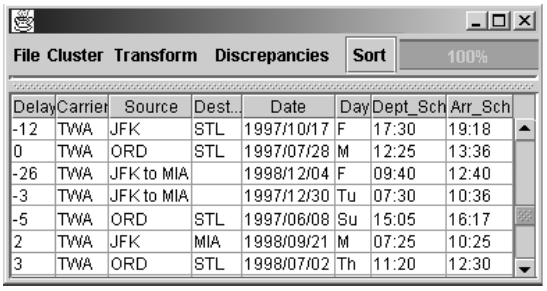
\includegraphics[width=0.7\textwidth]{figures/state-of-the-art/potters-wheel}
  \caption{Showing Potter's Wheel spreadsheet-like \gls{gui} approach\index{approach}. Transform operations are accessible via menu bar~\cite{Raman2001a}.}
  \label{fig:potters-wheel-screenshot}
\end{figure}


\subsection{PADS: A Domain-Specific Language Approach}

The system of \cite{Fisher2005} approaches\index{approach} the topic of transforming\index{transformation} large amounts of semi-structured data via a descriptive \textbf{\gls{dsl}}.
Consequently, it is lacking a visual-interactive\index{visual-interactive} component altogether and taken into consideration here for the sake of completeness and demonstrating a different solution view.
Users describe the data that is to be transformed\index{transformation} in the \gls{dsl}.
Then the \emph{PADS} compiler allows for generating (\textsc{C}-based) parser libraries and built-upon tools for further processing of such data.
The project was conducted at \emph{AT\&T} and focuses on specific data transformation\index{transformation} requirements of the company at that time.
Target output data formats are in particular \textsc{XML} and ones for loading the data into \gls{rdbms}es (i.e., \textsc{SQL}).
Mainly supported input formats are of \textsc{ASCII} (log files), binary (legacy networking protocols), and Cobol kind.
\\\\
Here is some exemplary web server access logs input data as shown in the paper:

{\tiny
  \begin{verbatim}
    207.136.97.49 - - [15/Oct/1997:18:46:51 -0700] "GET /tk/p.txt HTTP/1.0" 200 30
    tj62.aol.com - - [16/Oct/1997:14:32:22 -0700] "POST /scpt/dd@grp.org/confirm HTTP/1.0" 200 941
  \end{verbatim}
}

A \textbf{pro} argument for this approach\index{approach} is that the \gls{dsl} is relatively concise and easily graspable due to its declarative nature.
Furthermore, it frees its users from manually writing parsers and constructive tools as these are generated from the \gls{dsl} definitions of a concrete data format to work with.
Finally, the quality and range of tools can be improved and extended in a convenient way being quite independent from the generated parsers.

If we wanted to find a \textbf{con} argument here it could be that while being useful and a general step forward at the time of development, we believe that there are probably better ways to support certain kinds of end-users in these tasks, namely of the visual-interactive\index{visual-interactive} kind which we want to evaluate with this thesis after all.


\subsection{Microsoft BizTalk Schema Mapper Research}

In the approach\index{approach} of ~\cite{Robertson2005}, Microsoft's \emph{BizTalk} schema mapper application is attempted to be improved.
Main use case being visual and interactive support of mapping two differing \textsc{XML} schemas.
Moreover, the schemas are of considerable big size (i.e., thousands of elements in each schema) to be not processable in a usable way within the traditional \gls{ui}.
That is, too many connections between the schemas are shown in a too complex way to be useful.
To improve the \gls{ui} some \gls{infovis} techniques are applied (Figure~\ref{fig:biztalk-research-screenshot} presents a screenshot showing this).

As described by the authors, these techniques are:

\begin{itemize}
  \item \textbf{Highlight propagation:} \\(de-)emphasizing areas of interest within the mapping \gls{ui}
  \item \textbf{Auto-scrolling:} \\automatically scrolling to selected items (comparable to \glslink{ide}{IDEs}) etc.
  \item \textbf{Coalescing trees:} \\somewhat relating to highlight propagation hiding irrelevant nodes
  \item \textbf{Multi-select:} \\reasonable support for multi-selection of nodes concerted with general visualization
  \item \textbf{Incremental search:} live search results updating the \gls{ui} while typing
  \item \textbf{Bendable links:} enabling the user to see connections when actually overlayed
  \item \textbf{Focus on linked elements:} improved default behavior of up/down keys usage
\end{itemize}

The results are evaluated via a user study and have proven to be useful which can be seen as a \textbf{pro} argument here as well.

There is little to mention on the \textbf{con} side regarding the approach\index{approach} of ~\cite{Robertson2005} as it overall demonstrates an advancement in the area of interactive schema mapping.

\begin{figure}[h]
  \centering
  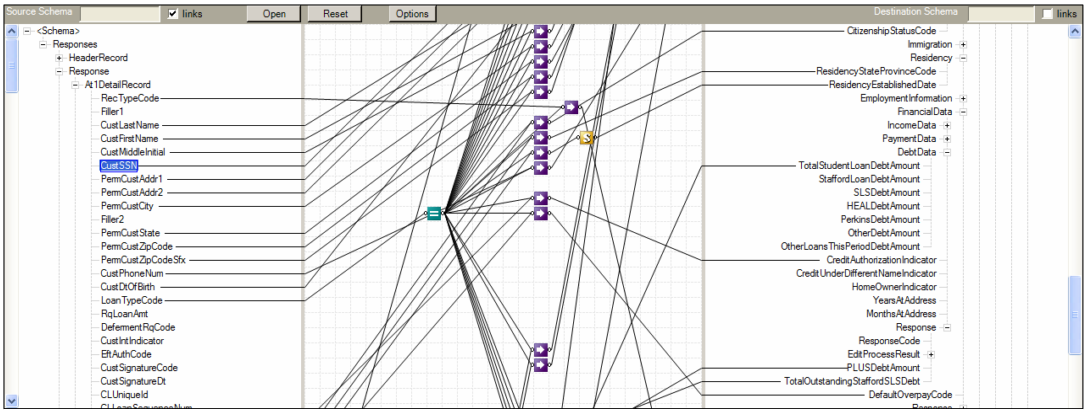
\includegraphics[width=1.0\textwidth]{figures/state-of-the-art/biztalk-research}
  \caption{BizTalk research GUI demonstrating some applied InfoVis techniques. On each vertical side of the visible pane, elements of a respective schema are represented by a tree-like structure. Mappings between them are visualized as arcs. Center nodes are used for displaying more complex (m:n-like) mappings~\cite{Robertson2005}.}
  \label{fig:biztalk-research-screenshot}
\end{figure}


\subsection{Clio: From Research Prototype to Industrial Tool}

In ~\cite{Haas2005} the authors outline the evolution of an IBM research prototype\index{prototype} to an industrial-strength tool.
\emph{Clio} is an application for descriptive specification of schema mappings.
It is mainly targeted towards \textsc{XML} and relational schemas (see Figure~\ref{fig:clio-screenshot}).
So, in this respect it is quite similar both by field and application to the aforementioned Microsoft \emph{``BizTalk''} schema mapper product, adding \gls{rdbms}/\textsc{SQL} mapping to the mix.
Mappings are represented by an abstract query graph allowing for translation of data transformations\index{transformation} into specific query languages.
This is what makes it interesting and distinguishing, again, when compared with Microsoft's \emph{BizTalk} schema mapping application.

Finally, the paper focuses on revisiting the architecture\index{architecture} and algorithms behind the software and then explains issues and solutions on the way to applying industrial usage.
Consequently, it is a useful real-world example of transferring science in practice.

\begin{figure}[h]
  \centering
  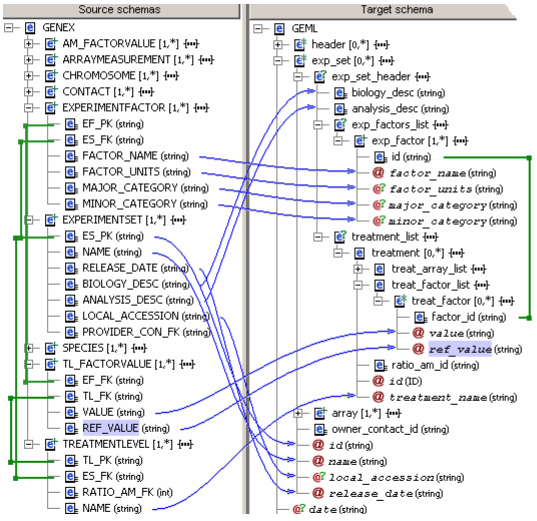
\includegraphics[width=0.66\textwidth]{figures/state-of-the-art/clio-grown-up}
  \caption{Clio GUI, also showing similarities with the MS BizTalk one. Consequentially, again, data schemas (this time from relational DBs, though) on the left and right-hand sides with mappings as arrowed lines~\cite{Haas2005}.}
  \label{fig:clio-screenshot}
\end{figure}


\subsection{Potluck: A Semantic Web Approach}

The research prototype\index{prototype} in \cite{Huynh2007} focuses on making heterogeneous \textbf{\emph{\gls{semanticweb}}} data accessible to casual users.
It provides a web interface for visual and interactive wrangling\index{wrangle} of data mainly relating to \gls{rdf}.
An interesting feature is allowing users to tag and visualize data with physical locations via a map view (see Figure~\ref{fig:potluck-map-screenshot}).
What is also interesting in this approach\index{approach} is its demonstration of increased interest respectively shift towards web technologies at that time.
Furthermore, it delivers some kind of preview how far web-based approaches\index{approach} would go in this area.
Plus, it illustrates the general trend in the direction of casual end-user applications (enabling non-expert users to operate actually complex tasks).

\begin{figure}[h]
  \centering
  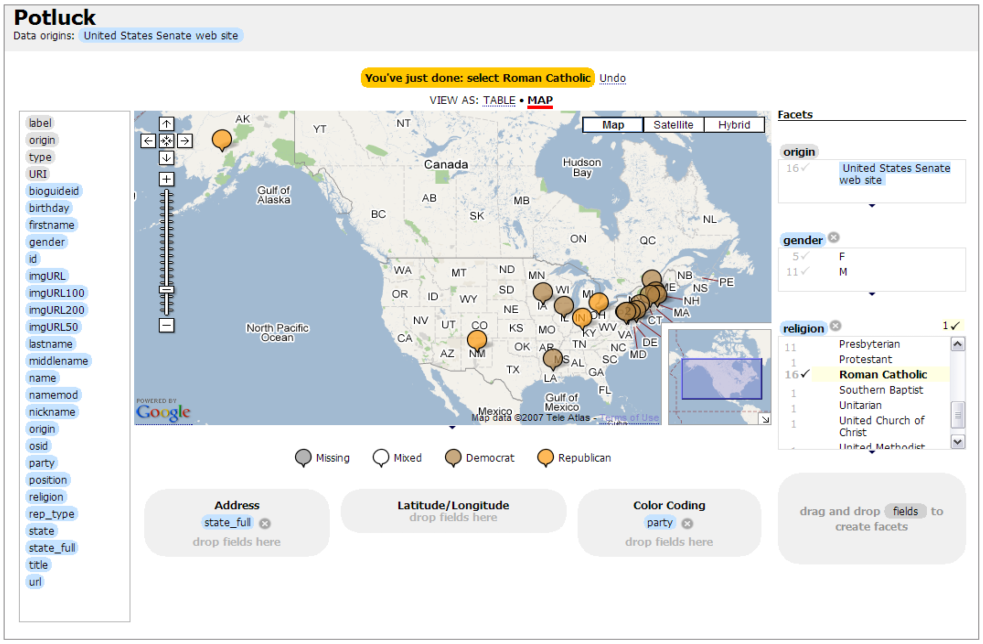
\includegraphics[width=1.0\textwidth]{figures/state-of-the-art/potluck-map-view}
  \caption{Potluck map view which can be seen as a back then innovative visualization in the field. Data is displayed geospatially~\cite{Huynh2007}.}
  \label{fig:potluck-map-screenshot}
\end{figure}

\newpage


\subsection{\gls{rnd} Veterans: DataWrangler \& OpenRefine}

The two systems that can be the seen to have set the benchmark in this space are:

\begin{enumerate}
  \item \textbf{\emph{DataWrangler}} (\emph{Stanford Visualization Group} research project\footnote{\textcolor{blue}{\href{http://vis.stanford.edu/wrangler/}{vis.stanford.edu/wrangler/}}})~\cite{Kandel2011a}
  \item \textbf{\emph{OpenRefine}} (open-sourced\footnote{\textcolor{blue}{\href{https://github.com/OpenRefine/OpenRefine}{github.com/OpenRefine/OpenRefine}}} product\footnote{\textcolor{blue}{\href{http://openrefine.org/}{openrefine.org}}} f.k.a. \emph{Google Refine} and \emph{Freebase Gridworks})
\end{enumerate}


\subsubsection{DataWrangler}

\emph{DataWrangler}, cf. Kandel et al. in~\cite{Kandel2011a}, is a web-browser-based application oriented towards a visually interactive approach\index{approach} (see Figure~\ref{fig:data-wrangler-screenshot}).
It contains an inference engine suggesting transforms\index{transformation}, plus, data cleaning sessions can be exported and reused as scripts.
The creators of the project meanwhile moved on to make a commercial product out of it, called \emph{Trifacta Wrangler}\footnote{\textcolor{blue}{\href{https://www.trifacta.com/products/wrangler/}{www.trifacta.com/products/wrangler/}}}.

One thing which is less supported by \emph{Wrangler} is full-control direct manipulation of data.
That is, it is more geared towards \gls{lpbd} than to deliberately changing the content of single values via direct input.

In addition to that, the \gls{ui} is limited which can also be ascribed to the web-based nature of the tool.
Things like not truly responsively, and richly interactive \gls{ux}, especially when the amounts of data that are to be wrangled\index{wrangle} grow.

DataWrangler was evaluated via a user study and has shown to improve productivity of \gls{datawrangling} tasks considerably.

Biggest \textbf{pro} arguments of the approach\index{approach}:

\begin{itemize}
  \item Interactively inferred suggested transforms\index{transformation}
  \item Rich collection of transforms\index{transformation} to be applied
  \item Shows the potential of pursuing the visual-interactive\index{visual-interactive} path
\end{itemize}

Main \textbf{con} argument is performance-wise constrained usefulness of the tool and its generally improvable \gls{ux}.
Also, no real charting support available, yet.

\begin{figure}[h]
  \centering
  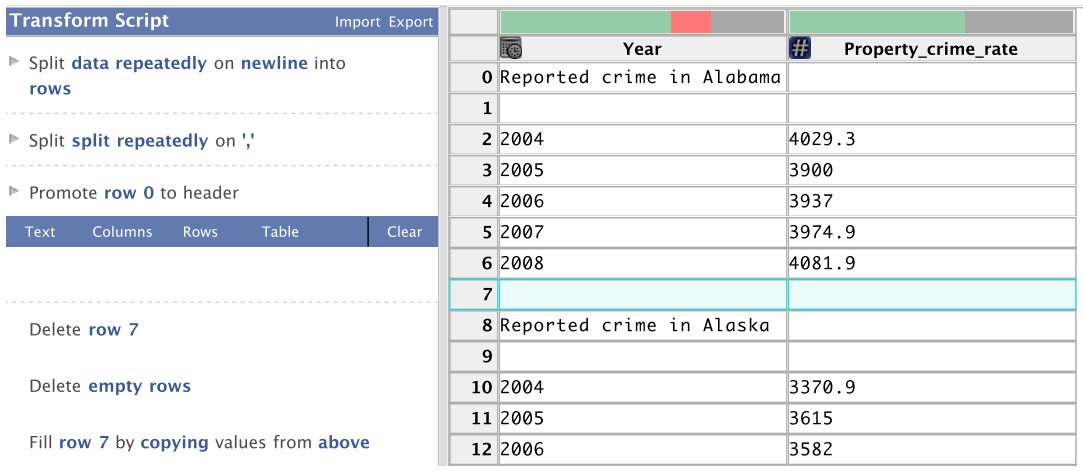
\includegraphics[width=1.0\textwidth]{figures/state-of-the-art/data-wrangler}
  \caption{DataWrangler \gls{ui} as a state of the art shaping, innovative approach\index{approach}. Data transform history and related suggestions are located on the left, tabular interaction pane on the right~\cite{Kandel2011a}.}
  \label{fig:data-wrangler-screenshot}
\end{figure}


\subsubsection{OpenRefine}

\emph{OpenRefine} is a browser-based application as well (but running locally on the user's machine, also due to data protection respectively privacy reasons).
It allows for direct manipulation of data (see Figure~\ref{fig:open-refine-screenshot}), yet, it supports less interaction-driven transform\index{transformation} operations than DataWrangler (which infers appropriate transformation\index{transformation} suggestions from solely pointing the cursor to data in a certain way).

A nice feature is its visual statistical\index{statistics} analytics of data distribution via histograms etc. ($\rightarrow$ \textbf{pro} argument).
But, on the \textbf{con} side, it generally lacks some data transformation\index{transformation} operations which are supported by DataWrangler (particularly reshaping-related, like un/folding -- extracting/merging specific parts of data within a column into/from additional ones).

\begin{figure}[h]
  \centering
  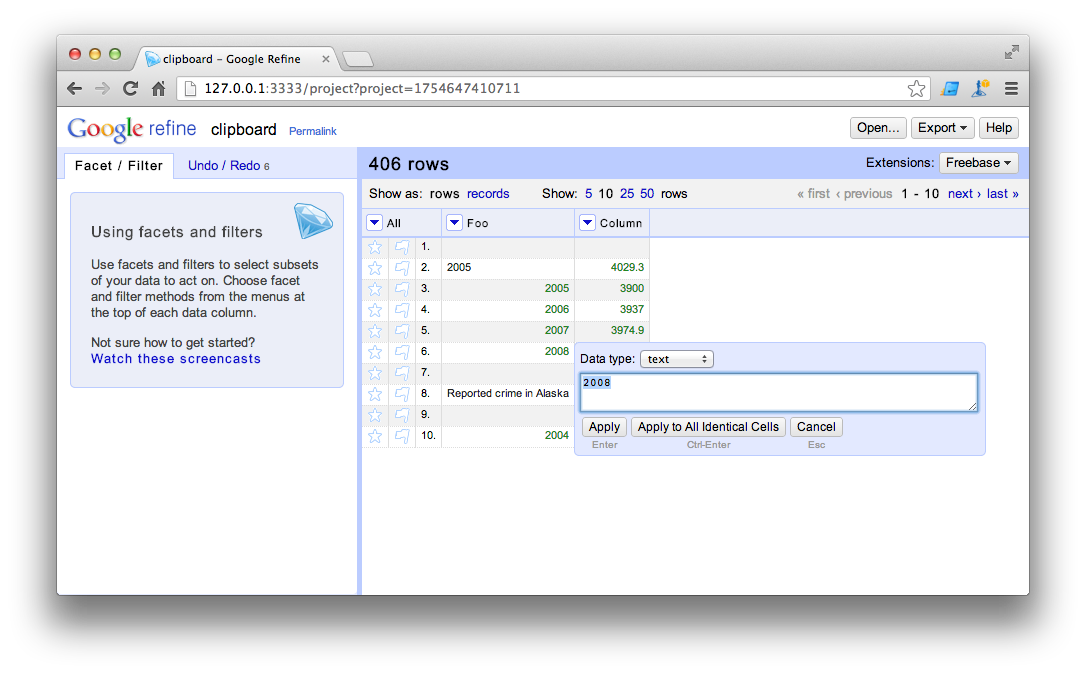
\includegraphics[width=1.0\textwidth]{figures/state-of-the-art/google-refine}
  \caption{Google/OpenRefine \gls{ui} in action, also offering direct manipulation of data. Again, as in DataWrangler, tabular respectively spreadsheet-like interface.}
  \label{fig:open-refine-screenshot}
\end{figure}


\subsection{Temporal Research: On Time Series Data}

The research prototype\index{prototype} in~\cite{Bernard2012} focuses specifically on time-series-based data.
It is tailored for joint usage of a domain and a \gls{datamining} expert.
Technically, a preprocessing pipeline is visual-interactively\index{visual-interactive} created and incrementally adjusted via the tool (see Figure~\ref{fig:time-series-research-screenshot}).

What is interesting here is the application of the domain on time series data.
Moreover, its pipeline-oriented workflow \gls{ui}, offering various statistical\index{statistics} visualizations, is a well-designed\index{design} asset.
Finally, the approach\index{approach} is evaluated by applying it to a case study delivering results proving it useful in its context.


\subsection{The Industry: Talend Open Studio}

Within the industry a well-known collection of enterprise tools is \emph{Talend Open Studio}\footnote{\textcolor{blue}{\href{https://www.talendforge.org/}{www.talendforge.org}}}.
This is an open source software suite with commercial support offerings.
Architecturally\index{architecture}, it is based on \emph{\textbf{Eclipse}} \gls{rcp}.
The product which can be used for \gls{datawrangling} is \emph{Talend Data Quality}\footnote{\textcolor{blue}{\href{https://www.talend.com/products/data-quality/}{www.talend.com/products/data-quality/}}} (see Figure~\ref{fig:talend-open-studio-screenshot} for its \gls{gui}).
It allows for interactive specification and execution of data transformations\index{transformation} with \textbf{visual charting aid}.
I.e., data at hand is visualized via meaningful charts while interactively manipulating it.


\subsection{An Innovative Approach\index{approach}: Kibana Timelion}

\emph{Kibana} is a product by the company \emph{Elastic} which is mainly geared towards visualizing data of their other product \emph{Elasticsearch} in an interactive fashion with charts.
As sort of a research project \emph{Timelion} was born (see \cite{web:Timelion} and Figure~\ref{fig:kibana-timelion}).
It allows for interactive exploration and transformation\index{transformation} of time series data with a programmatic, mathematical \gls{dsl} via a \gls{cli}.
Commands trigger chart visualizations accordingly.
The way these interaction methods are combined is rather unseen before.

Another Elastic product worth mentioning in our context is called \emph{Logstash}\footnote{\textcolor{blue}{\href{https://www.elastic.co/products/logstash}{www.elastic.co/products/logstash}}}.
This is basically a universal data processing engine with transformation\index{transformation} capabilities, historically focused on log event data, mainly driven by filter expressions written in \emph{Ruby}-like syntax.

\begin{figure}[h]
  \centering
  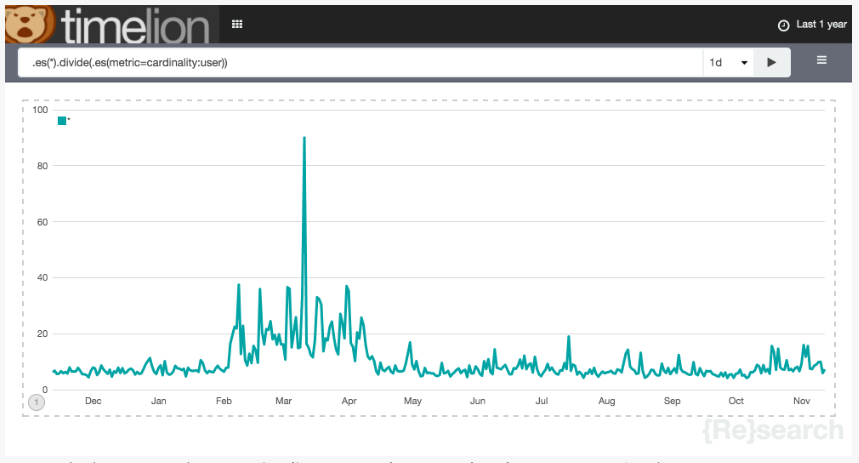
\includegraphics[width=1.0\textwidth]{figures/state-of-the-art/kibana-timelion}
  \caption{Kibana Timelion as an innovative approach to visual-interactively\index{visual-interactive} exploring and transforming time series data~\cite{web:Timelion}.}
  \label{fig:kibana-timelion}
\end{figure}


\subsection{Modern Data Science: Jupyter Notebooks}

\Gls{datascience} nowadays is commonly pursued with \emph{Jupyter Notebooks}\footnote{\textcolor{blue}{\href{https://jupyter.org/}{jupyter.org}}}.

These interactive notebooks are powered by a web-based application, often running locally and connecting to remote data sources.
The technology originally emerged from \emph{IPython}, an interactive \gls{cli} in \gls{repl} style.
It since has moved to the web and supports other popular \gls{datascience} languages, like \emph{R}, as well.
So one can make use of statistical\index{statistics} computations in a scripting manner, interactively creating according chart visualizations, potentially embedded in more standard textual sections.

\begin{figure}[h]
  \centering
  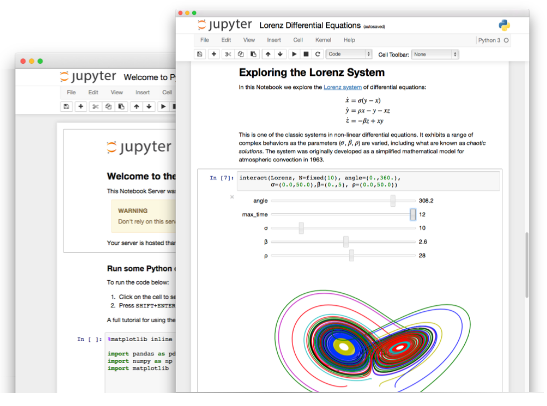
\includegraphics[width=0.85\textwidth]{figures/state-of-the-art/jupyter-notebooks}
  \caption{\Gls{datascience} with Jupyter Notebooks as advertised on their website.}
  \label{fig:jupyter-notebooks}
\end{figure}


\section{Comparison and Summary}

As shown by the presentation of related work, a diverse selection of approaches\index{approach} and tools can be found in this field. Yet, there are also quite some shared aspects to be recognized. For example, basic \gls{gui}s for visual-interactive\index{visual-interactive} schema mapping turned out to develop into pretty similar directions (compare, e.g., the mapping views of \emph{BizTalk} and \emph{Clio} projects as presented in Figure~\ref{fig:biztalk-research-screenshot} and~\ref{fig:clio-screenshot}).

Furthermore, the general \gls{ui} for displaying datasets in this area is spreadsheet-like (see \emph{Potter's Wheel}, \emph{DataWrangler}, \emph{OpenRefine}, and \emph{Talend}).
In addition to that, visual charting aids have started to be incorporated (particularly demonstrated by the more recent time series data related prototype\index{prototype} and commercial tools by \emph{Talend}).
Moreover, modern and innovative approaches\index{approach} are combining classic \emph{\gls{cli}} with scripting, and interactive charting in novel ways (see \emph{Kibana Timelion} and \emph{Jupyter Notebooks}).

Table~\ref{tab:comparison} provides a \textbf{comparison outline} of these projects as well as a preliminary \textbf{requirements list} for our approach.
It should be noted that ``visual interactivity'' is somewhat hard to measure therein, as some approaches\index{approach} lead into quite special directions.

According to these findings there seems to be a need for further research in visual-interactive\index{visual-interactive} aid, for example, via meaningful charts.
Gaps to be filled here are connected to applying interactive \gls{infovis} techniques in order to further improve support of \gls{datawrangling} tasks.
There are approaches\index{approach} already moving into this direction, yet, in particular interactive charting assistance has the potential to substantially facilitate wrangling\index{wrangle} tasks while still needing further research.
As it turns out, visual-interactively\index{visual-interactive} supporting \gls{datawrangling} tasks is currently still in its infancy.
While the general topic of \gls{datawrangling} is not new and quite some research and practice has been done in this field, combining it with \gls{gui}s offering decent \gls{ux} is relatively young.
Especially, incorporating visualization of the to-be-transformed\index{transformation} data and corresponding data transform\index{transformation} operations themselves via meaningful charts is something where further \gls{rnd} is required.

To this end, we are developing a research prototype\index{prototype}, called \emph{\textbf{TempMunger}}, facilitating a visual presentation of the data that enables a better and faster understanding of the data structure and where there is a need for transformation\index{transformation} as well as interactive charts for data manipulation and for giving immediate visual feedback of the transformation\index{transformation}.

\begin{sidewaysfigure}[h]
  \centering
  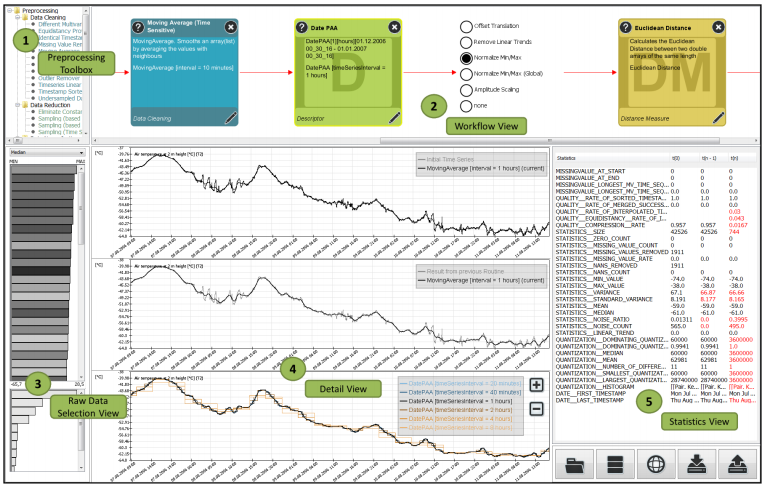
\includegraphics[width=0.95\textwidth]{figures/state-of-the-art/time-series-research}
  \caption{Time series research \gls{ui} with interesting pipeline-based approach (top pane). Various charts (main pane) visualize the data at hand (right pane)~\cite{Bernard2012}.}
  \label{fig:time-series-research-screenshot}
\end{sidewaysfigure}

\begin{sidewaystable}[htb]
  \centering
  \begin{tabular}{|l|c|c|c|c|c|c|c|}
    \hline \textbf{Project} & \textbf{Platform} & \textbf{Domain} & \textbf{GUI Richness} & \textbf{Visual Interactivity} & \textbf{Charts} & \textbf{Time-Oriented} & \textbf{Dashboard}  \\
    \hline
    \hline
    \hline \emph{Potter's Wheel}     & C++, Swing    & Generic         & Medium  & Medium   & No   & No      & No         \\
    \hline \emph{PADS}               & DSL Code, C   & Specific        & N/A     & N/A      & No   & No      & No         \\
    \hline \emph{BizTalk}            & Windows .NET  & Schema Mapping  & Medium  & Medium   & No   & No      & No         \\
    \hline \emph{Clio}               & Java Desktop  & Schema Mapping  & Medium  & Medium   & No   & No      & No         \\
    \hline \emph{Potluck}            & Web           & Semantic Web    & Low     & Medium   & No   & No      & No         \\
    \hline \emph{DataWrangler}       & Web           & Generic         & Medium  & Special  & No   & No      & No         \\
    \hline \emph{OpenRefine}         & Web           & Generic         & Medium  & High     & Yes  & Yes     & No         \\
    \hline \emph{Time Series}        & Unknown       & Specific        & High    & High     & Yes  & Yes     & Partially  \\
    \hline \emph{Talend}             & Eclipse RCP   & Generic         & High    & High     & Yes  & Unknown & Partially  \\
    \hline \emph{Kibana Timelion}    & Web           & Specific        & High    & Special  & Yes  & Yes     & No         \\
    \hline \emph{Jupyter Notebooks}  & Web           & Generic         & High    & Special  & Yes  & Yes     & No         \\
    \hline
    \hline \emph{\textbf{TempMunger}}  & \textbf{Desktop} (Web)  & \textbf{Generic}  & \textbf{High}  & \textbf{High}  & \textbf{Focus}  & \textbf{Highly} & \textbf{Focus}  \\
    \hline
  \end{tabular}
  \caption{Projects comparison serving as a starting point to derive basic requirements.}
  \label{tab:comparison}
\end{sidewaystable}

\begin{sidewaysfigure}[h]
  \centering
  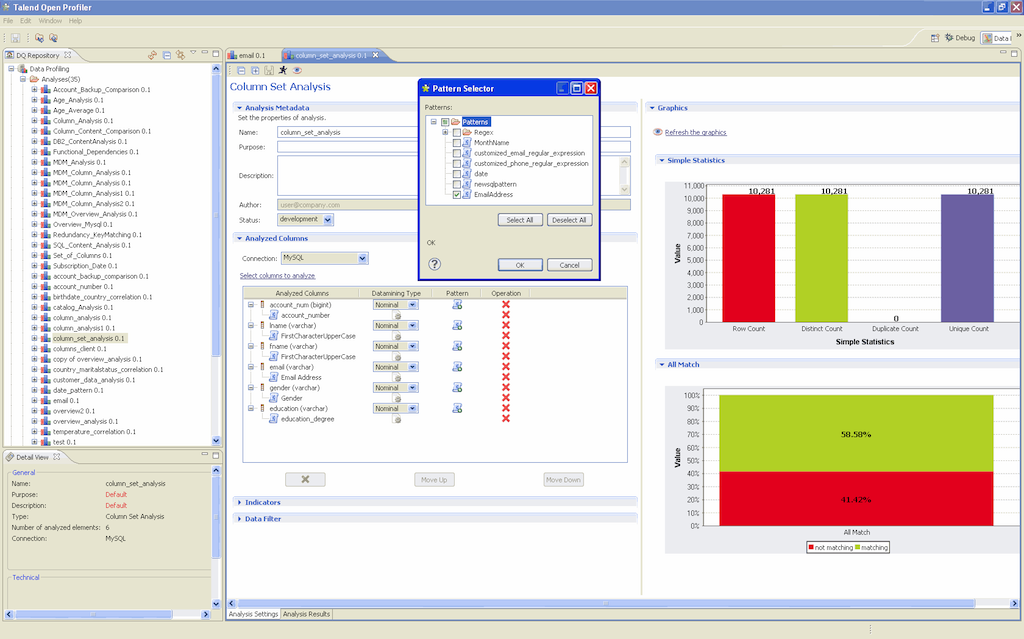
\includegraphics[width=0.95\textwidth]{figures/state-of-the-art/talend-open-studio}
  \caption{Talend Open Studio Data Quality \gls{gui} as an industry-standard solution based on Eclipse \gls{rcp}. Interactively manipulated data (on the left) by transformations (center) is visualized via charting support (right). Screenshot originally taken from product website.}
  \label{fig:talend-open-studio-screenshot}
\end{sidewaysfigure}


\subsection{Our Approach\index{approach}: TempMunger}

Where we are intending to excel with \emph{TempMunger} here is by bringing concepts from both \emph{DataWrangler} and \emph{OpenRefine} together with enhanced visual charting aid as well as our derived requirements (see Section~\ref{sec:requirements-list}) and improved \gls{ux}. The main kind of data to be wrangled\index{wrangle} in particular will be time-oriented\index{time-oriented}. So, focus will be laid on visual-interactive\index{visual-interactive} support of wrangling\index{wrangle} time-oriented\index{time-oriented} data.

More concrete, possible areas of improvement include:

\begin{itemize}
  \item Introduction of modern interaction patterns, like drag \& drop column merging
  \item Visualizing data structures via meaningful charts, presenting transform\index{transformation} suggestions
  \item Directly manipulative interaction with these charts to transform\index{transformation} underlying data
  \item Special focus on supporting time-oriented\index{time-oriented} data with meaningful charts and interactive transformations\index{transformation}
\end{itemize}

Further requirements are derived in Section~\ref{sec:requirements-list} and we expect that more reasonable functionality, features, and constraints will emerge from the iterative \emph{design\index{design} -- implementation -- evaluation} process of the thesis project.

In addition, we are going to tackle the following \gls{datawrangling} challenges as identified by \cite{Kandel2011b}:

\begin{enumerate}
  \item \emph{Diagnosing data problems visually}
  \item \emph{Visualizing ``raw'' data}
  \item \emph{Visual assessment and specification of automated methods}
  \item \emph{Living with dirty data} (visually; i.e., how to display erroneous data best)
\end{enumerate}

While these \gls{infovis} topics are merely directed towards data profiling, we extend upon this by applying it to transformations\index{transformation} connected to \gls{datawrangling}.
\\\\
To sum it up with our main research question, stated once again:

\emph{\textbf{How can we support \gls{datawrangling} with \gls{va} techniques?}}



%%%%%%%%%%%%%%%%%%%%%%%%%%%%%%%%%%%%%%%%%
\chapter{Design and Implementation}
\label{ch:design+impl}
%%%%%%%%%%%%%%%%%%%%%%%%%%%%%%%%%%%%%%%%%

\newacronym{jvm}{JVM}{Java Virtual Machine}
\newacronym{rest}{ReST}{Representational State Transfer}
\newacronym{dx}{DX}{Developer Experience}
\newacronym{vcs}{VCS}{Version Control System}
\newacronym{scm}{SCM}{Source Code Management}
\newacronym{fs}{FS}{File System}
\newacronym{ci}{CI}{Continuous Integration}
\newacronym{saas}{SaaS}{Software as a Service}
\newacronym{rdd}{RDD}{Resilient Distributed Dataset}
\newacronym{soc}{SoC}{Separation of Concerns}
\newacronym{dom}{DOM}{Document Object Model}
\newacronym{spa}{SPA}{Single Page Application}
\newacronym{seo}{SEO}{Search Engine Optimization}
\newacronym{hmr}{HMR}{Hot Module Replacement}
\newacronym{svg}{SVG}{Scalable Vector Graphics}
\newacronym{tf-idf}{TF-IDF}{Term Frequency -- Inverse Document Frequency}
\newacronym{utc}{UTC}{Coordinated Universal Time}
\newacronym{gmt}{GMT}{Greenwich Mean Time}


\section{Requirements Analysis}

This is a vital part and first step of our methodology leading to a proposed solution.


\subsection{UX Personas}

In order to derive a meaningful list of design\index{design} requirements we make use of an instrument from designing\index{design} products called \gls{ux} personas.

It has been pioneered for usage with software development by Cooper~\cite{Cooper2004}. The basic idea is to come up with some stereotypical ``personalities'' described by certain characteristics which represent our target user groups.
An important aspect is the potential creation of empathy with our future users.

Each of these personas is, typically, illustrated with a profile picture and at least a firstname.
The notion is to create some degree of familiarity and identifiability for the \gls{ux} designer\index{design} and other parties involved in the design\index{design} process.
Furthermore, usually, a persona is equipped with some demographical coordinates, some sort of tagline which serves as an executive summary, enhanced with background info, and motivations.
All of this information is normally pointed and rather skimped.
It should support in easily creating a vivid idea and image of the different users of the product in design\index{design}.

Finally, scenarios or user stories briefly describe ways in which these particular user types would use the imaginary product.
In the end, it is important the resulting personas can also be physically tangible -- for instance, printed out on cards and pinned onto a whiteboard.
Personas are a valuable tool for subsequent design\index{design} of \gls{ui} and interactions.

Table~\ref{tab:ux-personas} provides a high-level overview of the personas we came up with for our prototypical\index{prototype} software, focusing on skill set distribution.
As one can see, persona skills range from overall highly to overall lowly skilled as well as individuals with focus on certain different skills.
This makes for an interesting foundation as, all in all, quite a disperse set of potential users has to be catered for. The following pages contain our personas themselves.
The profile pictures were created with an online avatar tool\footnote{\textcolor{blue}{\href{http://avachara.com/avatar/}{avachara.com/avatar/}}}.

\begin{table}
  \centering
  \begin{tabular}{ccccccc}
    \toprule
    \emph{Skills}      & Hugo             & Alice          & Bob              & John    & Jane           & Walter  \\
    \midrule
    Technical          & \textbf{low}  & \textbf{high}  & low              & low     & high           & low     \\
    Scientific         & medium        & \textbf{high}  & \textbf{low}     & medium  & high           & high    \\
    Data-Related       & medium        & high           & \textbf{medium}  & medium  & \textbf{high}  & medium  \\
    Temporal Interest  & medium        & high           & \textbf{low}     & high    & \textbf{high}  & high  \\
    \bottomrule
  \end{tabular}
  \caption{UX personas skill summary and comparison. Edge entries in \textbf{bold}.}
  \label{tab:ux-personas}
\end{table}

\subsection{Requirements List} \label{sec:requirements-list}

Through the creation of our personas we were able to properly visualize and dissect corresponding requirements for our prototype\index{prototype}.
Consequently, we have derived these:

\begin{itemize}
  \item \textbf{R1:} The prototype\index{prototype} must be capable of loading and working with diverse datasets
  \item \textbf{R2:} Moreover, it must be intuitive for casual users (i.e., less technically expertized)
  \item \textbf{R3:} Yet, some shortcuts for rather power users should be supported as well
  \item \textbf{R4:} Focus of our approach\index{approach} has to be on visual-interactive\index{visual-interactive} charting aid
  \item \textbf{R5:} These charts must be centered on applying time-oriented\index{time-oriented} data transformations\index{transformation}
  \item \textbf{R6:} Plus, they should provide extraordinary visual overview of the dataset at hand
  \item \textbf{R7:} Thus, focus has to be put on choosing most effective and efficient visualizations
  \item \textbf{R8:} Furthermore, interactively exploring data must be conveniently possible
  \item \textbf{R9:} A more traditional tabular editor should be available with direct manipulation
  \item \textbf{R10:} Editing time-oriented\index{time-oriented} data should be supported by specific \gls{ui} controls
  \item \textbf{R11:} Data quality issues need to be easily identifiable and effectually addressable
  \item \textbf{R12:} Conveniently spotting data anomalies respectively outliers should be possible
  \item \textbf{R13:} Concrete time-oriented\index{time-oriented} data transformation\index{transformation} operations to be supported:
  \begin{itemize}
    \item Data cleaning regarding missing and erroneous values
    \item Normalization concerning points in time and intervals
    \item Merging columns in an intuitive visual-interactive\index{visual-interactive} way
    \item Formatting cleanup, e.g., inconsistencies or conversion
  \end{itemize}
\end{itemize}


\subsection{Hugo}


\includegraphics[scale=0.5]{figures/requirements/persona-avatar-hugo}

\subsubsection{Demographics}

\begin{itemize}
    \item Age: 35
    \item Location: Vienna, Austria
    \item Job: Business Analyst
    \item Expertise: Marketing \& Statistics\index{statistics}
\end{itemize}

\subsubsection{Tagline}

\textit{``I need to quickly filter out erroneous data from market survey results.''}

\subsubsection{Background}

\begin{itemize}
    \item Studied business administration focusing on marketing and specializing in statistics\index{statistics}
    \item Some years of working experience in the industry
    \item Responsible for pointing out business opportunities through analyses\index{analysis}
\end{itemize}

\subsubsection{Motivations}

\begin{itemize}
    \item Wants to see the ``big picture''
    \item Doesn't want to ``lose'' any time
\end{itemize}

\subsubsection{Scenarios (User Stories)}

\begin{itemize}
    \item Got huge amounts of messy real-world data from various market surveys
    \item Wants to ``scan'' this data quickly for using it in market/business analyses\index{analysis}
    \item Often data is time-oriented\index{time-oriented}, as it denotes market-related developments over time
\end{itemize}


\subsection{Alice}

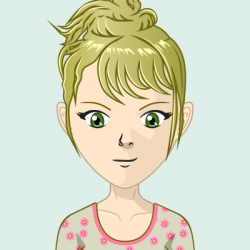
\includegraphics[scale=0.5]{figures/requirements/persona-avatar-alice}

\subsubsection{Demographics}

\begin{itemize}
    \item Age: 31
    \item Location: Vienna, Austria
    \item Job: Academic Researcher
    \item Expertise: Mathematics \& Statistics\index{statistics}
\end{itemize}

\subsubsection{Tagline}

\textit{``I'm interested in spending less time wrangling\index{wrangle} datasets suitable for analysis\index{analysis}.''}

\subsubsection{Background}

\begin{itemize}
    \item Studied mathematics with a focus on statistics\index{statistics} resulting in a research position in the field (post-doctoral)
    \item Special focus of the research group is time-oriented\index{time-oriented} data, being involved in various international projects
\end{itemize}

\subsubsection{Motivations}

\begin{itemize}
    \item Wants to analyze huge datasets, often containing flawed data
    \item She would rather spend time on analysis\index{analysis} than preparation
\end{itemize}

\subsubsection{Scenarios (User Stories)}

\begin{itemize}
    \item Got various sample time-oriented\index{time-oriented} datasets and wants to analyze the data
    \item Furthermore, wrangling\index{wrangle} should take less effort to apply Occam's razor
\end{itemize}


\subsection{Bob}

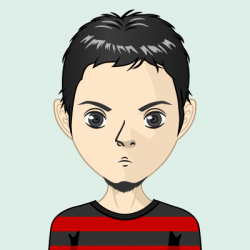
\includegraphics[scale=0.5]{figures/requirements/persona-avatar-bob}

\subsubsection{Demographics}

\begin{itemize}
    \item Age: 34
    \item Location: Graz, Austria
    \item Job: Journalist
    \item Expertise: Journalism \& Politics
\end{itemize}

\subsubsection{Tagline}

\textit{``I would like to be able to handle messy data for analysis\index{analysis} to be used in my articles.''}

\subsubsection{Background}

\begin{itemize}
    \item Graduate of communication studies with a specialization in politics
    \item Worked for several online news agencies
\end{itemize}

\subsubsection{Motivations}

\begin{itemize}
    \item Is held back from doing real ``data journalism'' due to lack of technical skills
    \item Would get into this kind of journalism if tools were better suited to his needs
\end{itemize}

\subsubsection{Scenarios (User Stories)}

\begin{itemize}
    \item Got an idea for a current news story based on some quite untidy political/economic data which is often of time-oriented\index{time-oriented} nature
    \item Is able to conveniently verify justification of story based on respective analysis\index{analysis} of wrangled\index{wrangle} data
\end{itemize}


\subsection{John}

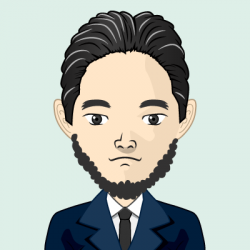
\includegraphics[scale=0.5]{figures/requirements/persona-avatar-john}

\subsubsection{Demographics}

\begin{itemize}
    \item Age: 40
    \item Location: Salzburg, Austria
    \item Job: Political Analyst
    \item Expertise: Politics \& Statistics\index{statistics}
\end{itemize}

\subsubsection{Tagline}

\textit{``I want to conveniently and visually prepare vast amounts of public poll data for analysis\index{analysis}.''}

\subsubsection{Background}

\begin{itemize}
    \item Studied political sciences with a focus on statistics\index{statistics} (Ph.D.)
    \item Works for news agencies, especially analyzing electoral situations
\end{itemize}

\subsubsection{Motivations}

\begin{itemize}
    \item Strong need to be able to get lots of data from various polls into unified schema with as little hassle as possible
    \item Is not particularly technically skilled or interested, just wants to get the data to be able analyzing it
\end{itemize}

\subsubsection{Scenarios (User Stories)}

\begin{itemize}
    \item Electoral poll data, consequently, mainly temporal natured, from various sources needs to get prepared respectively unified for analyzing
    \item Uses the visual-interactive\index{visual-interactive} tool being able to get the job done in a convenient way
\end{itemize}


\subsection{Jane}

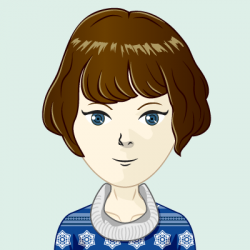
\includegraphics[scale=0.5]{figures/requirements/persona-avatar-jane}

\subsubsection{Demographics}

\begin{itemize}
    \item Age: 37
    \item Location: Munich, Germany
    \item Job: Industrial Researcher
    \item Expertise: Biology \& Statistics\index{statistics}
\end{itemize}

\subsubsection{Tagline}

\textit{``I need a quick(er) and more reliable way to experiment with biological test data.''}

\subsubsection{Background}

\begin{itemize}
    \item Graduated in bio engineering
    \item Works at a pharmaceutical company testing new ways of synthesizing cosmetics
\end{itemize}

\subsubsection{Motivations}

\begin{itemize}
    \item Currently, the whole roundtrip of setting up test labs and analyzing results is cumbersome and takes much time
    \item Wants to be able to iterate in a quicker mode of operation by improving on wrangling\index{wrangle} test data applicable for actual analysis\index{analysis}
\end{itemize}

\subsubsection{Scenarios (User Stories)}

\begin{itemize}
    \item Is able to reduce testing roundtrips by using the visual-interactive\index{visual-interactive} tool for making time series test data useful for analysis\index{analysis}
    \item Based on experience and results from previous iterations she is able to decrease overall throughput time even more
\end{itemize}


\subsection{Walter}

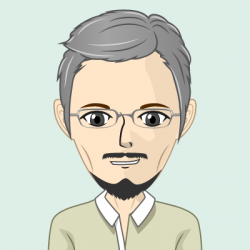
\includegraphics[scale=0.5]{figures/requirements/persona-avatar-walter}

\subsubsection{Demographics}

\begin{itemize}
    \item Age: 46
    \item Location: Vienna, Austria
    \item Job: Medical Doctor
    \item Expertise: Diabetes
\end{itemize}

\subsubsection{Tagline}

\textit{``I want to be able to conveniently visualize temporal therapy data provided by patients.''}

\subsubsection{Background}

\begin{itemize}
    \item Studied medicine, graduating cum laude
    \item Works at special center focusing on diabetics treatment
\end{itemize}

\subsubsection{Motivations}

\begin{itemize}
    \item Often, therapy data provided by patients is rather messy, that is, concerning missing respectively erroneous values, formatting, ...
    \item Wants to be able to visualize data to get to see the ``real'' picture
\end{itemize}

\subsubsection{Scenarios (User Stories)}

\begin{itemize}
    \item Using the tool he is able to reduce time spent on getting time-series-based therapy data provided by his patients ready for analysis\index{analysis} and can focus on actually analyzing
    \item Might even encourage (at least some of) his patients to use the tool themselves to further reduce overhead
\end{itemize}


\section{Design of UI and Interactions}

For designing\index{design} the \gls{ui} and interactions we have created mockups a.k.a. wireframes~\cite{Garrett2011}.

\subsection{UI Mockups}

The design\index{design} of our prototype\index{prototype} should meet our list of requirements. To this end, we created a number of mockups to be able to easily refine our designs\index{design}.

We have created our \gls{ui} mockups using \emph{Balsamiq\footnote{\textcolor{blue}{\href{https://balsamiq.com/}{balsamiq.com}}}} as productive tool.
An important aspect of wireframing is that it should be convenient creating the mockups.
One needs to be able to quickly iterate on ideas and throw away things which did not lead into the right direction.
Often, simply pencil and paper are being used which is already a good way to get to some first scribbles.
A quite common mistake is to skip proper wireframing and jump to design\index{design} screens immediately.
Most of the power within the creative design\index{design} process and flow is lost this way as design\index{design} screens take considerably more effort in producing them.
Consequently, iterating on these is usually more sluggish and throwing results away rather avoided.

The following pages contain our resulting wireframed mockups including some descriptions and further explanations regarding their functionality and respective underlying reasoning.
Mockups were created iteratively and evaluated in qualitative feedback loops until satisfying results have been achieved, that went into prototypical\index{prototype} implementation.

\subsubsection{Design Process}

While iteratively designing\index{design} with the help of mockups we constantly refined our ideas, adapting our approach\index{approach}, and trashing things that did not work out as expected.\\
Some material thereby discovered and/or changed:

\begin{itemize}
  \item Foremost, pie charts are, mostly, not useful in our context of transforming time-oriented\index{time-oriented} data
  \item On the other hand, bar charts are well suited to communicate quantities (e.g., of different table entries)
  \item Line charts, as commonly used for time series data, are not being emphasized on in our approach\index{approach}, mainly since we have found calendar heatmap visualizations to be superior for our use case, as our approach is generally not constrained to time series data but should be suitable for any time-oriented data
  \item Normalization functionality consciously left rather vague, to be fleshed out when actually developing the prototype\index{prototype}
  \item Modal dialogs containing interactive charts make sense for certain actions
  \item Visualizing the context of two different columns next to each other for exploratory comparison is beneficial
  \item A browser-based application is sufficient and a dedicated desktop one not needed in this case
\end{itemize}


\subsubsection{Upload Dialog}

\begin{figure}[h]
  \centering
  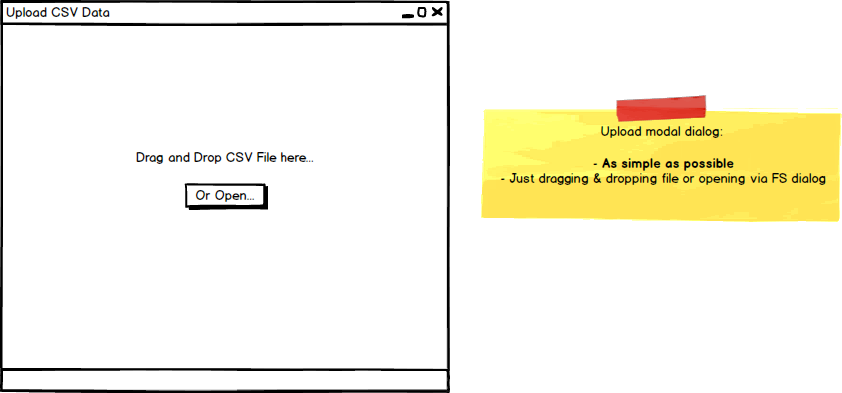
\includegraphics[width=1.125\textwidth]{figures/design/mockup-0}
  \caption{UI mockup of the upload dialog.}
  \label{fig:mockup-0}
\end{figure}

Naturally, the first \gls{ui} component we have designed\index{design} is the one which feeds the application with data to operate on:
the upload dialog (see Figure~\ref{fig:mockup-0}).

\begin{itemize}
  \item \textbf{Description}
  \begin{itemize}
    \item The main goal here was simplicity
    \item Consequently, truly simple dialog
    \item An area for dropping off file
  \end{itemize}
  \item \textbf{Reasoning}
  \begin{itemize}
    \item As it is central to the application, uploading has to be really simple
    \item Thus, with as little effort as possible
    \item That is, affordance has to be intuitive
  \end{itemize}
\end{itemize}

The idea regarding interaction is that as soon as a file is selected, the upload commences automatically, giving visual feedback of its progress to the user via according animation effects, disappearing as soon as it is finished.


\subsubsection{Table Editor}

\begin{figure}[h]
  \centering
  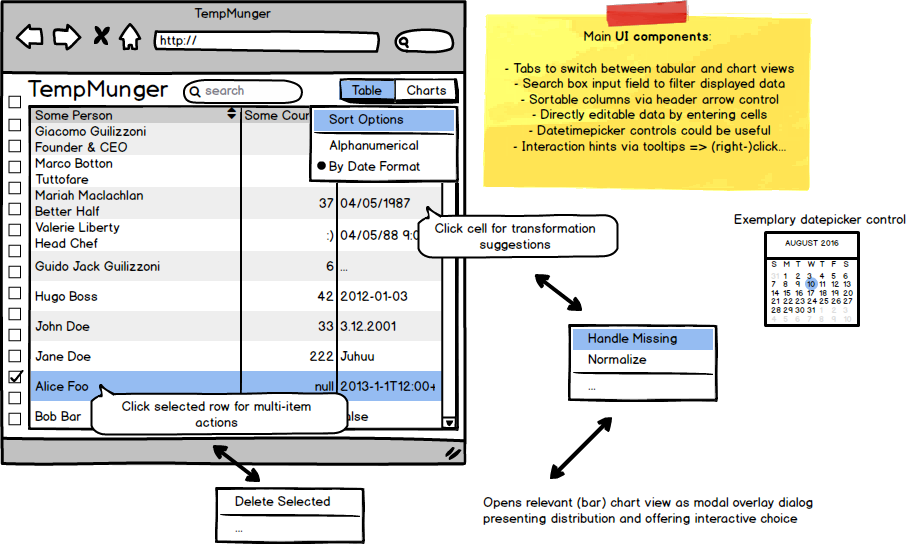
\includegraphics[width=1.2\textwidth]{figures/design/mockup-1}
  \caption{UI mockup of the table editor.}
  \label{fig:mockup-1}
\end{figure}

The table editor page (see Figure~\ref{fig:mockup-1}) has been designed\index{design} to be one of the two main pages of the application, the charts page being the second one, intuitively accessible via tabbed navigation in the upper right of the screen.

\begin{itemize}
  \item \textbf{Description}
  \begin{itemize}
    \item Enables direct manipulation editing of data
    \item Supports multi-row actions via check box selection
    \item Various search, sorting, and filtering options are available
    \item Provides menu access to further and more specialized dialogs
  \end{itemize}
  \item \textbf{Reasoning}
  \begin{itemize}
    \item The table editor is a well-known \gls{ui} metaphor for this use case
    \item Many users are familiar with editing tabular data from MS Excel \& co.
    \item It supplies the user with a straightforward and efficient mode of interaction
  \end{itemize}
\end{itemize}


\subsubsection{Missing Values Dialog}

\begin{figure}[h]
  \centering
  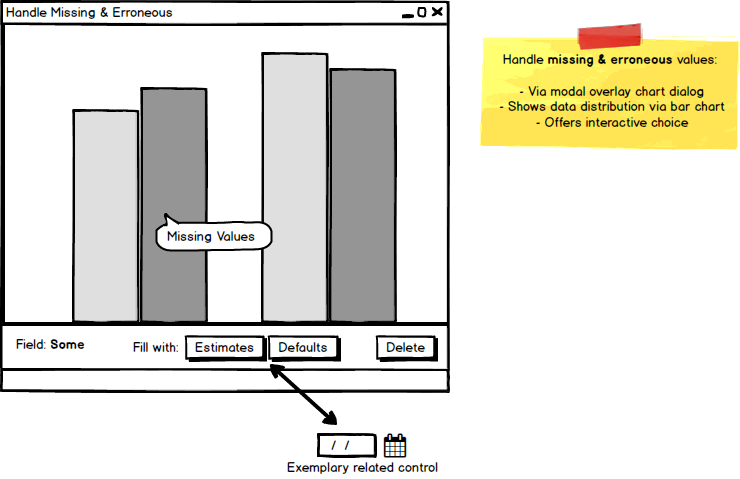
\includegraphics[width=1.12\textwidth]{figures/design/mockup-2}
  \caption{UI mockup of the missing values dialog.}
  \label{fig:mockup-2}
\end{figure}

The missing values dialog (see Figure~\ref{fig:mockup-2}) has been designed\index{design} to be opened from the table editor page via according menu access.

\begin{itemize}
  \item \textbf{Description}
  \begin{itemize}
    \item Concrete shape of chart not 100\% clear at this point
    \item Most probably, bar chart -- possibly, a horizontal one
    \item User is able to fill missing value entries or delete them
    \item Options provided are filling them with estimates or defaults
  \end{itemize}
  \item \textbf{Reasoning}
  \begin{itemize}
    \item Bar charts are capable of communicating distributions well
    \item Another possibility would be pie charts, but they are proven to be misleading
    \item To quote Tufte~\cite{Tufte2001}, p. 178: \emph{``Given
  their low density and failure to order numbers along a
  visual dimension, \textbf{pie charts should never be used}.''}\footnote{Cf. \textcolor{blue}{\href{https://www.edwardtufte.com/bboard/q-and-a-fetch-msg?msg\_id=00018S}{www.edwardtufte.com/bboard/q-and-a-fetch-msg?msg\_id=00018S}}}
  \end{itemize}
\end{itemize}


\subsubsection{Normalization Dialog}

\begin{figure}[h]
  \centering
  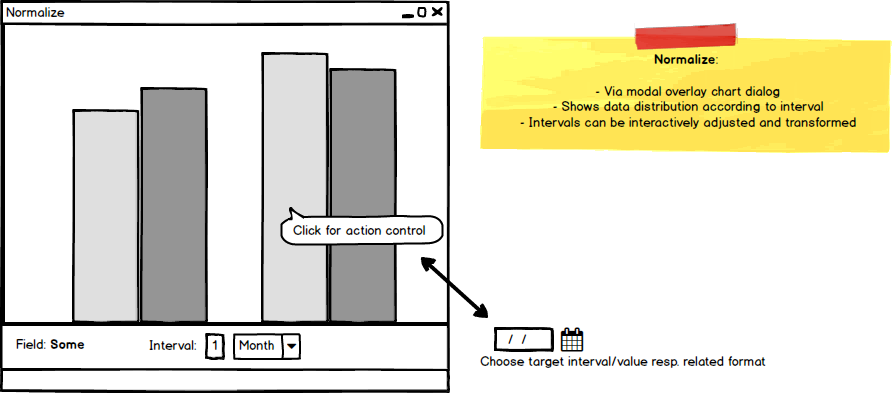
\includegraphics[width=1.2\textwidth]{figures/design/mockup-3}
  \caption{UI mockup of the normalization dialog.}
  \label{fig:mockup-3}
\end{figure}

The interval-focused normalization dialog (see Figure~\ref{fig:mockup-3}) is meant to be accessible via menu from the table editor page, too.

\begin{itemize}
  \item \textbf{Description}
  \begin{itemize}
    \item Its purpose is supposed to be enabling a user to normalize temporal intervals
    \item For batch-wise transforming\index{transformation} values of entries within a certain timespan
    \item Chart visualization is rather unclear at this stage
    \item Probably, bar chart as well -- but rather vertical one
    \item Interaction via point and click, including with chart
  \end{itemize}
  \item \textbf{Reasoning}
  \begin{itemize}
    \item The use case being worth covering became evident while gathering requirements
    \item Consequently, we will experiment with supporting it via meaningful interactive chart visualization
    \item Concrete characteristics will be shaped while iterative development itself
    \item Most probably, our color scheme of the chart visualization will be within neutral, plain gray to black range
    \item Since explicit coloring should only be used when it can communicate and, hence, convey meaning to the user, being intention-revealing, that is
    \item So, in the case of Figure~\ref{fig:mockup-2} it may make sense to use a noticeable color
  \end{itemize}
\end{itemize}


\subsubsection{Outlier Detection Alerting}

\begin{figure}[h]
  \centering
  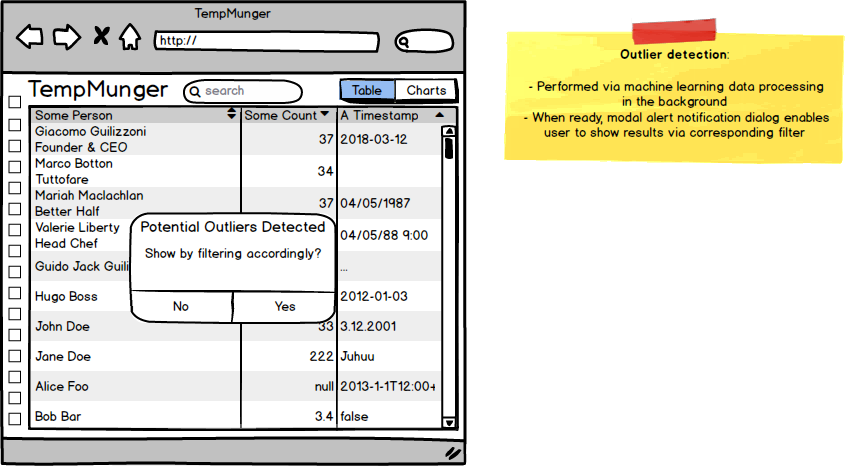
\includegraphics[width=1.1\textwidth]{figures/design/mockup-4}
  \caption{UI mockup of the outlier detection info alert.}
  \label{fig:mockup-4}
\end{figure}

When outliers are detected we need to show that to the user (see Figure~\ref{fig:mockup-4}).
As we intend to apply \glslink{ml}{machine learning} for this purpose, we need some way to do so without sacrificing good \gls{ux}.

\begin{itemize}
  \item \textbf{Description}
  \begin{itemize}
    \item Therefore, a simple modal dialog overlay is chosen
    \item It offers the user to display detected potential outliers
    \item When the user accepts, views are filtered accordingly
  \end{itemize}
  \item \textbf{Reasoning}
  \begin{itemize}
    \item Corresponding \gls{ml} processing has to happen in the background
    \item This is due to its potentially longer lasting computation time
    \item Consequently, informing the user about results has to be as unobtrusive as possible without interruption
    \item So, it should definitely not interfere with the current workflow, goals, and tasks of the user
    \item Thus, we intend to make use of an overlay which does not block the \gls{ui} and stays around for later use, more like an interactive notification-style message
  \end{itemize}
\end{itemize}


\subsubsection{Table Column Merging}

\begin{figure}[h]
  \centering
  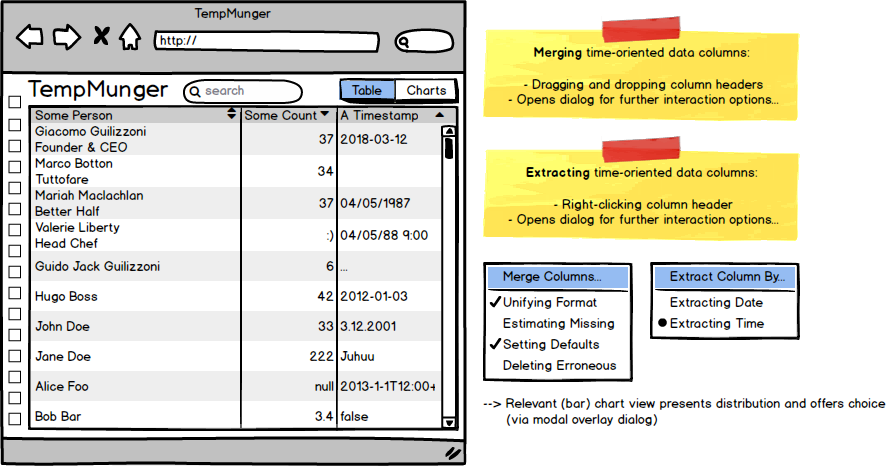
\includegraphics[width=1.175\textwidth]{figures/design/mockup-5}
  \caption{UI mockup of merging table columns via drag \& drop.}
  \label{fig:mockup-5}
\end{figure}

An interesting idea is to enable merging time-oriented\index{time-oriented} data columns via drag \& drop interaction metaphor (see Figure~\ref{fig:mockup-5}).

\begin{itemize}
  \item \textbf{Description}
  \begin{itemize}
    \item So when dragging a temporal column unto another, a related merging operation should be initiated
    \item The initial idea is to offer optional choice regarding the merge via a menu then
    \item Options like what to do with missing values and how to merge values in general
    \item Another idea is enabling column extraction via drag \& drop as well, still somewhat vague, though
  \end{itemize}
  \item \textbf{Reasoning}
  \begin{itemize}
    \item Many users are familiar with the basic kind of this interaction from spreadsheet applications like Excel
    \item Consequently, when indicating via according cursor on hover it is likely users will give it a spin
    \item Corresponding coloring of drop targets while dragging would be helpful to support the user with the interaction
  \end{itemize}
\end{itemize}


\subsubsection{Charts Page}

\begin{figure}[h]
  \centering
  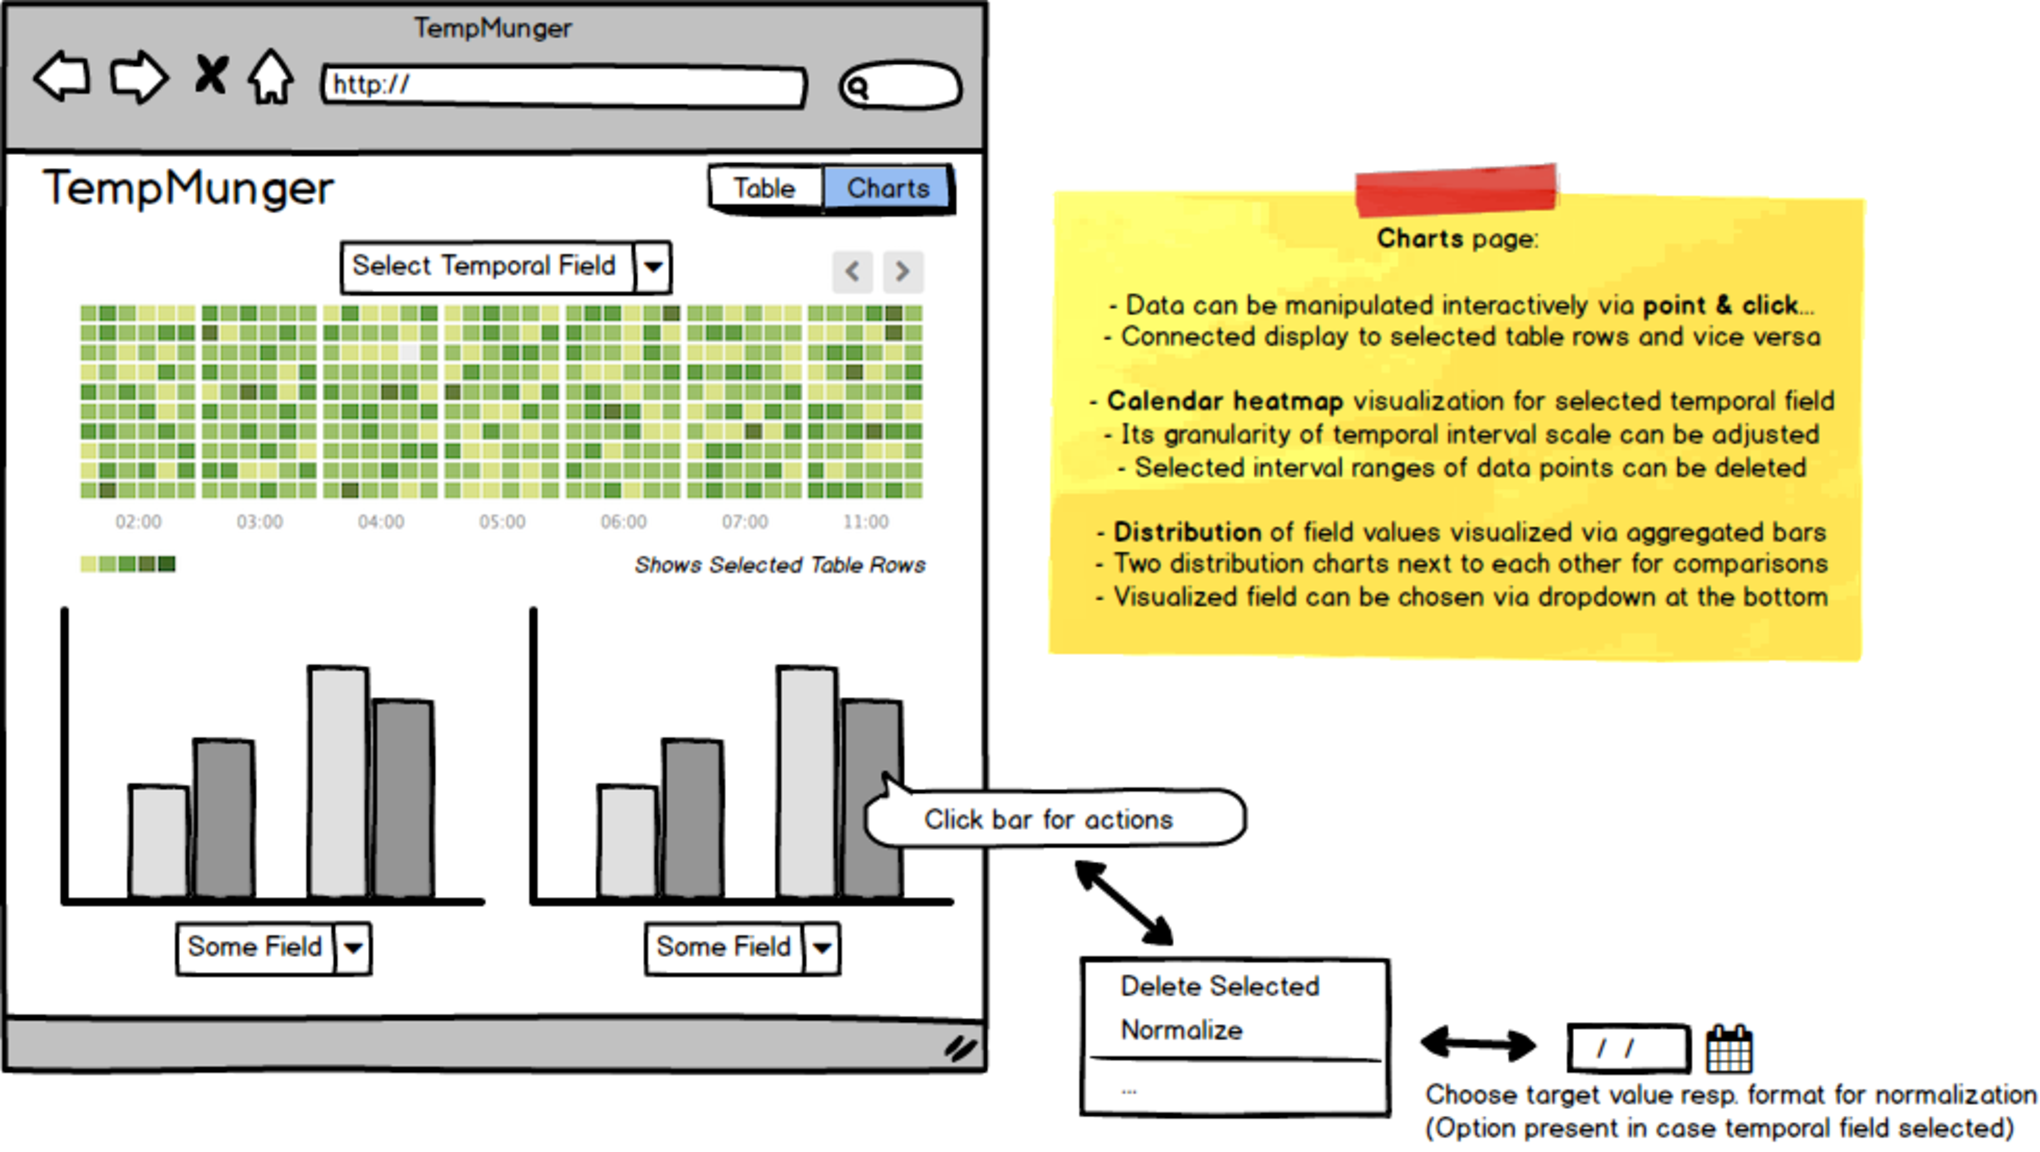
\includegraphics[width=1.1\textwidth]{figures/design/mockup-6}
  \caption{UI mockup of the charts page including calendar heatmap visualization.}
  \label{fig:mockup-6}
\end{figure}

The charts page is the second of the two main pages of the application, next to the initial table editor one.

\begin{itemize}
  \item \textbf{Description}
  \begin{itemize}
    \item It is headed by an interactive calendar heatmap visualization
    \item Below, two distribution bar charts are next to each other
    \item Controls allow interacting with the charts, plus their items should be interactive
    \item Table editor filtering is intended to be interconnected with charts page views
  \end{itemize}
  \item \textbf{Reasoning}
  \begin{itemize}
    \item Calendar heatmap visualizations are particularly useful for displaying time-oriented\index{time-oriented} data distributions
    \item Densities of data therein are usually visualized via appropriate color scheming, popularly ranging in the green spectrum
    \item Histogram-like bar charts are useful for viewing data distributions in general
    \item Having two of the latter next to each other is great for comparisons, interactive exploration, and discovery
  \end{itemize}
\end{itemize}


\section{Iterative Prototyping}

Following the creation of our \gls{ui} mockups and agreeing that a satisfiable state had been reached, we started with implementing the corresponding prototypical\index{prototype} software.

So, we developed in an agile manner, meaning close contact and collaboration with the ``client'', in this case the assisting thesis advisor.
Plus, developing respective parts of the application iteratively, chunk by chunk, preferably with short iteration cycles.
While developing new features there were also regular short phases in between, where focus was laid on bug fixing, cleanup, and polishing of existing things.

Therefore, we have set up a live testing environment, easily accessible for the client, regularly shipping changes, and gathering feedback to be incorporated as promptly as possible.
Technical details regarding the setup are described in Appendix~\ref{ch:appendix-a}.

As workflows in this project were particularly lean and lightweight, no special issue management software was used.
It generally sufficed to make use of simple tools like \emph{Wunderlist}\footnote{\textcolor{blue}{\href{https://www.wunderlist.com/}{www.wunderlist.com}}}, \emph{Simplenote}\footnote{\textcolor{blue}{\href{https://simplenote.com/}{simplenote.com}}}, and email communication for tracking, planning as well as discussing todos, tasks, and issues.
Additionally, from time to time when felt necessary and considered potentially fruitful, personal meetings were held.
Mainly for hands-on demoing and reviewing purposes, plus, talking about direction-giving decisions.

This process was followed until the prototype\index{prototype} eventually reached feature-completeness.


\section{TempMunger}

This section goes into some details regarding the implemented prototype\index{prototype} itself.
Extensive documentation of related software design\index{design} and architecture\index{architecture} can be found in Appendix~\ref{ch:appendix-a}.


\subsection{Implementation Details}

As \gls{ide}, \emph{IntelliJ IDEA\footnote{\textcolor{blue}{\href{https://www.jetbrains.com/idea/}{www.jetbrains.com/idea/}}}} was used. \\
For conveniently reloading compiled code on the backend without requiring server restarts, \emph{JRebel\footnote{\textcolor{blue}{\href{https://zeroturnaround.com/software/jrebel/}{zeroturnaround.com/software/jrebel/}}}} was employed.
On the frontend, a technique called \emph{\gls{hmr}} is fulfilling similar tasks.
\emph{Redux DevTools\footnote{\textcolor{blue}{\href{http://extension.remotedev.io/}{extension.remotedev.io}}}} is a useful Google Chrome browser extension when developing Redux/React apps, and \emph{PageSpeed\footnote{\textcolor{blue}{\href{https://developers.google.com/speed/pagespeed/}{developers.google.com/speed/pagespeed/}}}} for adhering to website performance best practices.
Cross-browser development as well as responsiveness for mobile devices were not part of the thesis prototype\index{prototype}. Though, at least basic support may be present due to libraries used.
So the application is primarily optimized and tested to run in a Google Chrome \textbf{desktop} browser.

The source code might be made public as open source software at some point in time, most likely on GitHub.


\subsubsection{Elasticsearch Aggregations}

Foundational background regarding \gls{ir} and the search engine technology used for our prototype\index{prototype} can be found in Appendix~\ref{ch:appendix-b}.
Its software architecture is covered in Appendix~\ref{ch:appendix-a}.
Aggregations are a powerful way in which \emph{Elasticsearch} supports real-time analytics.
They are used extensively throughout our application.
The general idea is to aggregate occurrences of certain values in buckets with corresponding counts.
Most of the charts implemented in our solution rely heavily on these. Moreover, Elasticsearch aggregations can be nested which renders lots of analytical variety possible.
Thus, we are storing field values non-analyzed for aggregation as well as analyzed for full-text search purposes.

\subsubsection{Our Data Model/Storage}

The basic data model is a rather schema-less one.
So, Elasticsearch is enabled to figure out data types automatically on first indexing of respective data when uploading a dataset to the application.
Uploading data issues wiping the index before storing it.
Generally, there are two data types made available to our solution, either text or temporal.
For recognizing temporal data, various related formats are specified for parsing attempts.
Our data model is also quite lenient when it comes to values which fail parsing, simply ignoring the failure and storing the value at hand anyway.
This way missing or erroneous values can be treated separately.
See Appendix~\ref{ch:appendix-c} for a list of supported formats.
Temporal values are uniformly stored in our Elasticsearch index in \emph{\gls{utc}} timezone respectively \emph{\gls{gmt}}.
When load as local date/time values on the frontend these are converted making use of timezone offset calculations.

\subsubsection{On Spark RDDs}

As explained in Appendix~\ref{ch:appendix-a}, \emph{Apache Spark} is operating on \gls{rdd}s.
In our prototype\index{prototype}, these are being filled with data by querying Elasticsearch.
Extensive caching and pre-loading of data is applied to boost performance.
More concretely, for instance, the use case can be to transform\index{transformation} all dataset entries within a certain timespan for a specific temporal field to a specified other temporal value.

\subsubsection{Via Elasticsearch Bridge}

This is being accomplished via an Elasticsearch/Spark bridge, as described in Section~\ref{sec:es-hadoop}.
Thus, a Spark context can be configured to connect to an Elasticsearch cluster.
In the end, one can transparently operate on \gls{rdd}s with Spark's functional programming model\footnote{\textcolor{blue}{\href{https://spark.apache.org/docs/latest/programming-guide.html\#transformations}{spark.apache.org/docs/latest/programming-guide.html\#transformations}}}.

\subsubsection{With Seamless Interop}

The interop is, all in all, quite seamless.
Especially also concerning Kotlin code calling the ES-Hadoop connector Java \textsc{API} as well as Spark's underlying Scala one when necessary.
Loading data from and writing it back to Elasticsearch is mostly transparent.

\begin{figure}[h]
  \centering
  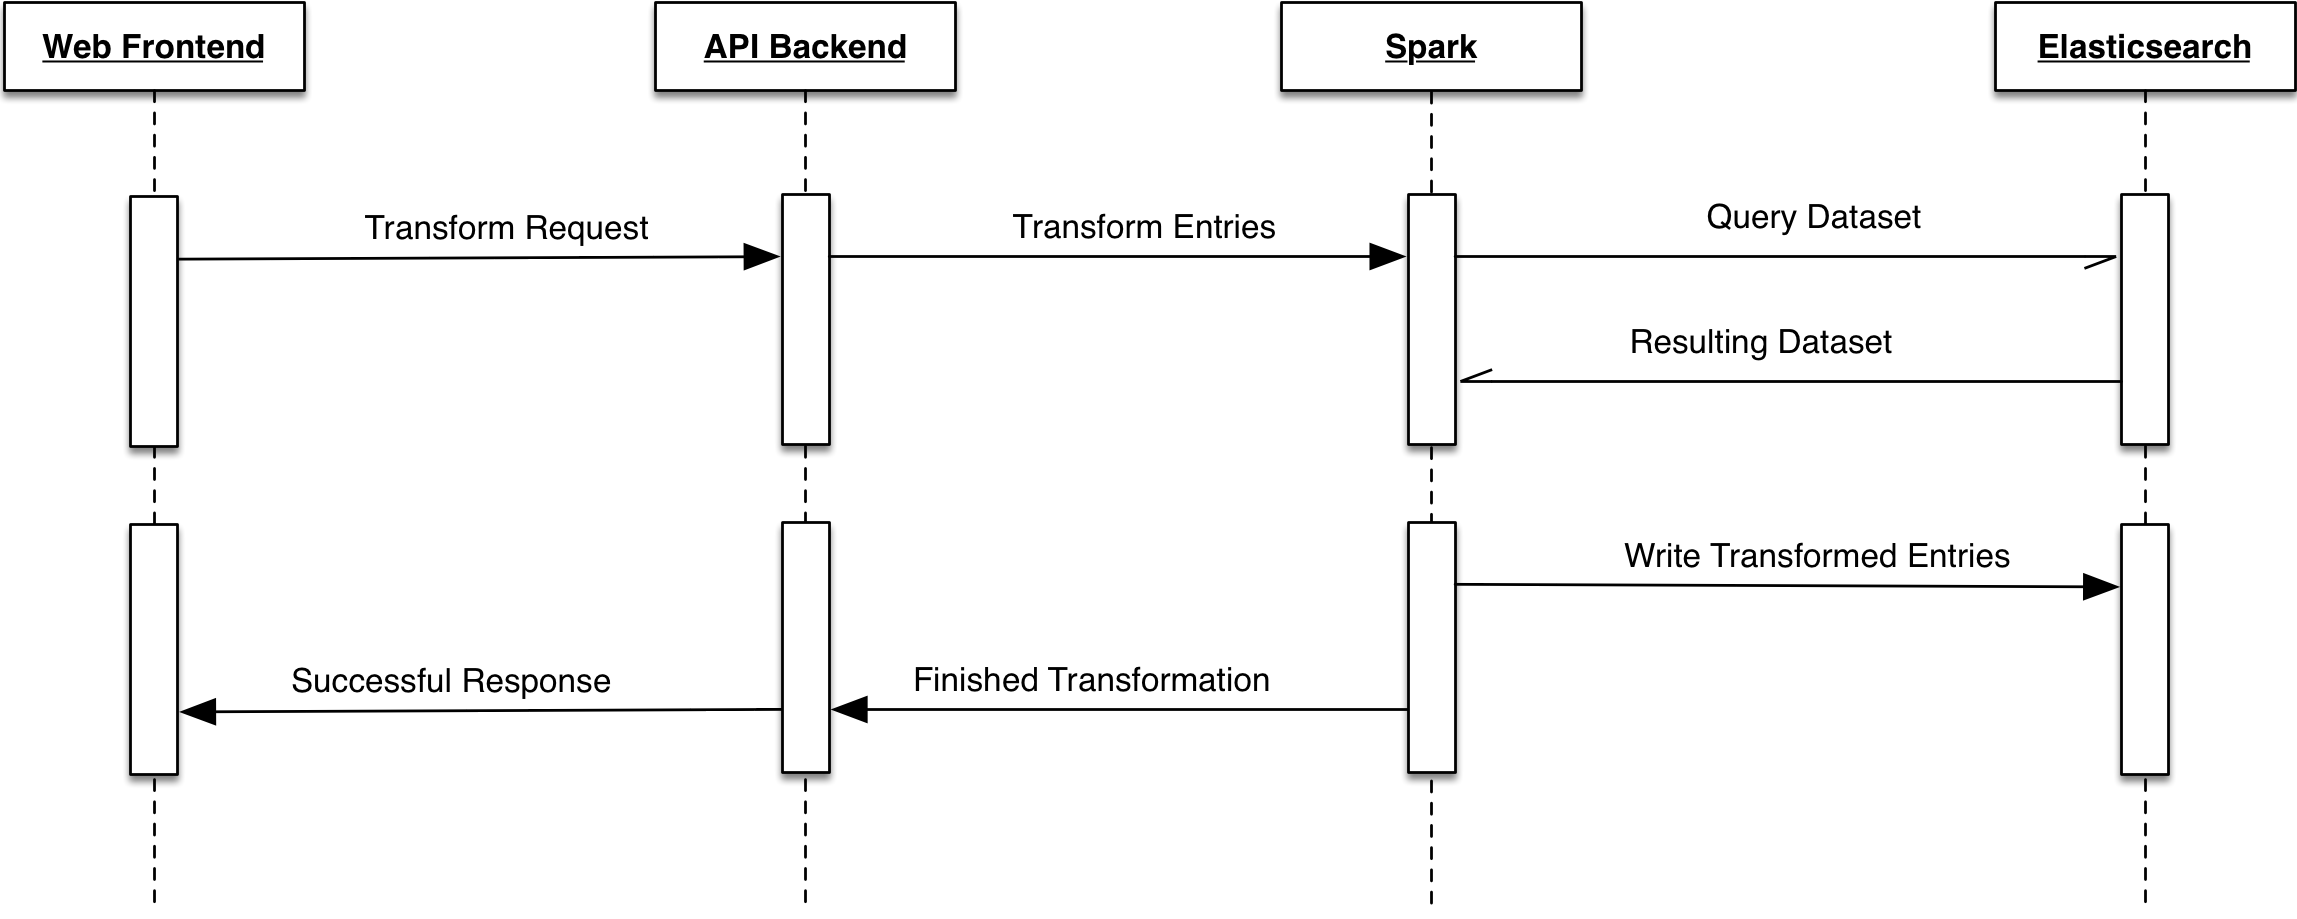
\includegraphics[width=1.05\textwidth]{figures/implementation/transformation-sequence}
  \caption{Sequence diagram showing the general data transformation flow.}
  \label{fig:transformation-sequence}
\end{figure}


\subsection{Features of TempMunger}

Our prototype\index{prototype} possesses the following main, high-level features regarding time-oriented\index{time-oriented} data, primarily focusing on visual-interactive\index{visual-interactive}, and particularly charting support:

\begin{itemize}
  \item \textbf{Transformations}\index{transformation}
  \begin{itemize}
    \item \textbf{Direct manipulation} via \gls{ui} controls
    \item \textbf{Cleaning} of missing and erroneous values
    \item \textbf{Normalization} concerning:
    \begin{itemize}
      \item Points in time
      \item Intervals
    \end{itemize}
    \item \textbf{Deletion} of rows
    \item \textbf{Merging} of columns
    \item \textbf{Formatting} cleanup
  \end{itemize}
  \item \textbf{Outlier detection}
  \item \textbf{Visual overview}
\end{itemize}

Furthermore, a more traditional \textbf{tabular editor} is available as known from spreadsheet applications like, most prominently, Microsoft Excel. Users are used to the underlying interaction metaphor and, consequently, it makes sense as a foundation to build upon.

\subsection{Transformations}

A central part of the approach\index{approach} is transformation\index{transformation} of time-oriented\index{time-oriented} data.
Generally, this is being achieved by making use of Apache Spark processing of Elasticsearch data.
As mentioned above, transformation\index{transformation} operations include \textbf{cleaning}, \textbf{normalization}, and \textbf{merging}.
Figure~\ref{fig:transformation-sequence} is presenting the general underlying flow via a sequence diagram.


\subsection{Outlier Detection}

Our prototype\index{prototype} applies some \gls{ml} techniques for its temporal outlier detection component.


\subsubsection{K-Means Clustering}

This is a popular algorithm of \emph{unsupervised learning}, i.e., \gls{ml} which does not rely on manual classification input, but rather classifies recognized patterns autonomously.

Formula~\ref{eq:k-means} represents its core principle, partitioning real vectorized observations $x$ into $k$ class cluster sets $S$ by calculating mean distances to respective centers ($\mu$ being the mean of points in $S_i$), generally computationally applying statistics\index{statistics} to pattern recognition:

\begin{equation}
\argmin_{S} \sum_{i=1}^{k} \sum_{x \in S_{i}} \|x - \mu_{i}\|^{2}
\label{eq:k-means}
\end{equation}

The following explains how this can be used for anomaly respectively outlier detection.

\subsubsection{Outlier Detection Usage}

The algorithm applied for our outlier detection component, basically, works as depicted in Algorithm~\ref{alg:temp-outlier-detection}.

A peculiar detail of our approach\index{approach} is that there is no dedicated test set of ``new'' data.
This is due to the fact there is only one dataset available at a time with no additional data coming in to extend it.
Thus, after training on a randomly split set, the whole dataset is used as test set, in the end, leading to overall satisfactory results.
Moreover, we are limiting the number of classes to be clustered to two.
Hence, our simple heuristic for determining an outlier class is to take the one of the two with fewer members.
When there is only one class, it is assumed no outliers could be detected.

\subsubsection{The Temporal Dimension}

Our use case revolves around finding outliers in time-oriented\index{time-oriented} data.
Figure~\ref{fig:outlier-detection-sequence} shows the basic, related flow with a sequence diagram.
In principle, we are using all time-oriented\index{time-oriented} data values available in the dataset at hand for vectorizing the observations to be input to clustering.
Therefore, the corresponding epoch millisecond values are used and if a certain value cannot be parsed it is substituted with a max. large number.
Consequently, missing and erroneous values are likely to be subsequently tagged as outliers as well.

\newpage


\begin{algorithm}
  \KwIn{A set of temporal field names $\varphi$ and a corresponding RDD (dataset) $\delta$}
  \KwOut{An RDD $\pi$ consisting of pairs of document ID to cluster class value}
  Vectorize dataset $\delta$ using field values via $\varphi$, see conditional (ll. 2-6)\;
  \eIf{a field value can be parsed as temporal}{
    Use its epoch milli value\;
  }{
    Use max. large number\;
  }
  Get training set $\tau$ from dataset $\delta$ via random split of $0.9 : 0.1$\;
  Create predictive model $\mu$ from vectors $\vec{x}$ of training set $\tau$\;
  $\to$ $k$-$means$ clustering yielding $2$ classes in $20$ iterations and $3$ parallel runs\;
  Predict points of dataset $\delta$ via model $\mu$, resulting in RDD $\pi$, see loop (ll. 11-14)\;
  \For{each point $\in$ dataset $\delta$}
  {
    Predict cluster class via model $\mu$\;
    Add result to RDD $\pi$\ via map op;
  }
  \Return{RDD $\pi$;}
  \caption{Temporal Outlier Detection}
  \label{alg:temp-outlier-detection}
\end{algorithm}

To further describe key points of the algorithm:\\
First, the dataset at hand is vectorized in order to enable applying it for clustering.
Then, a training set is generated from it via random split.
After that, a predictive model is created from the training set.
Afterwards, the dataset at hand is predictively clustered via model.
Finally, potential outliers are determined via aforementioned, simple heuristic.

\begin{figure}[h]
  \centering
  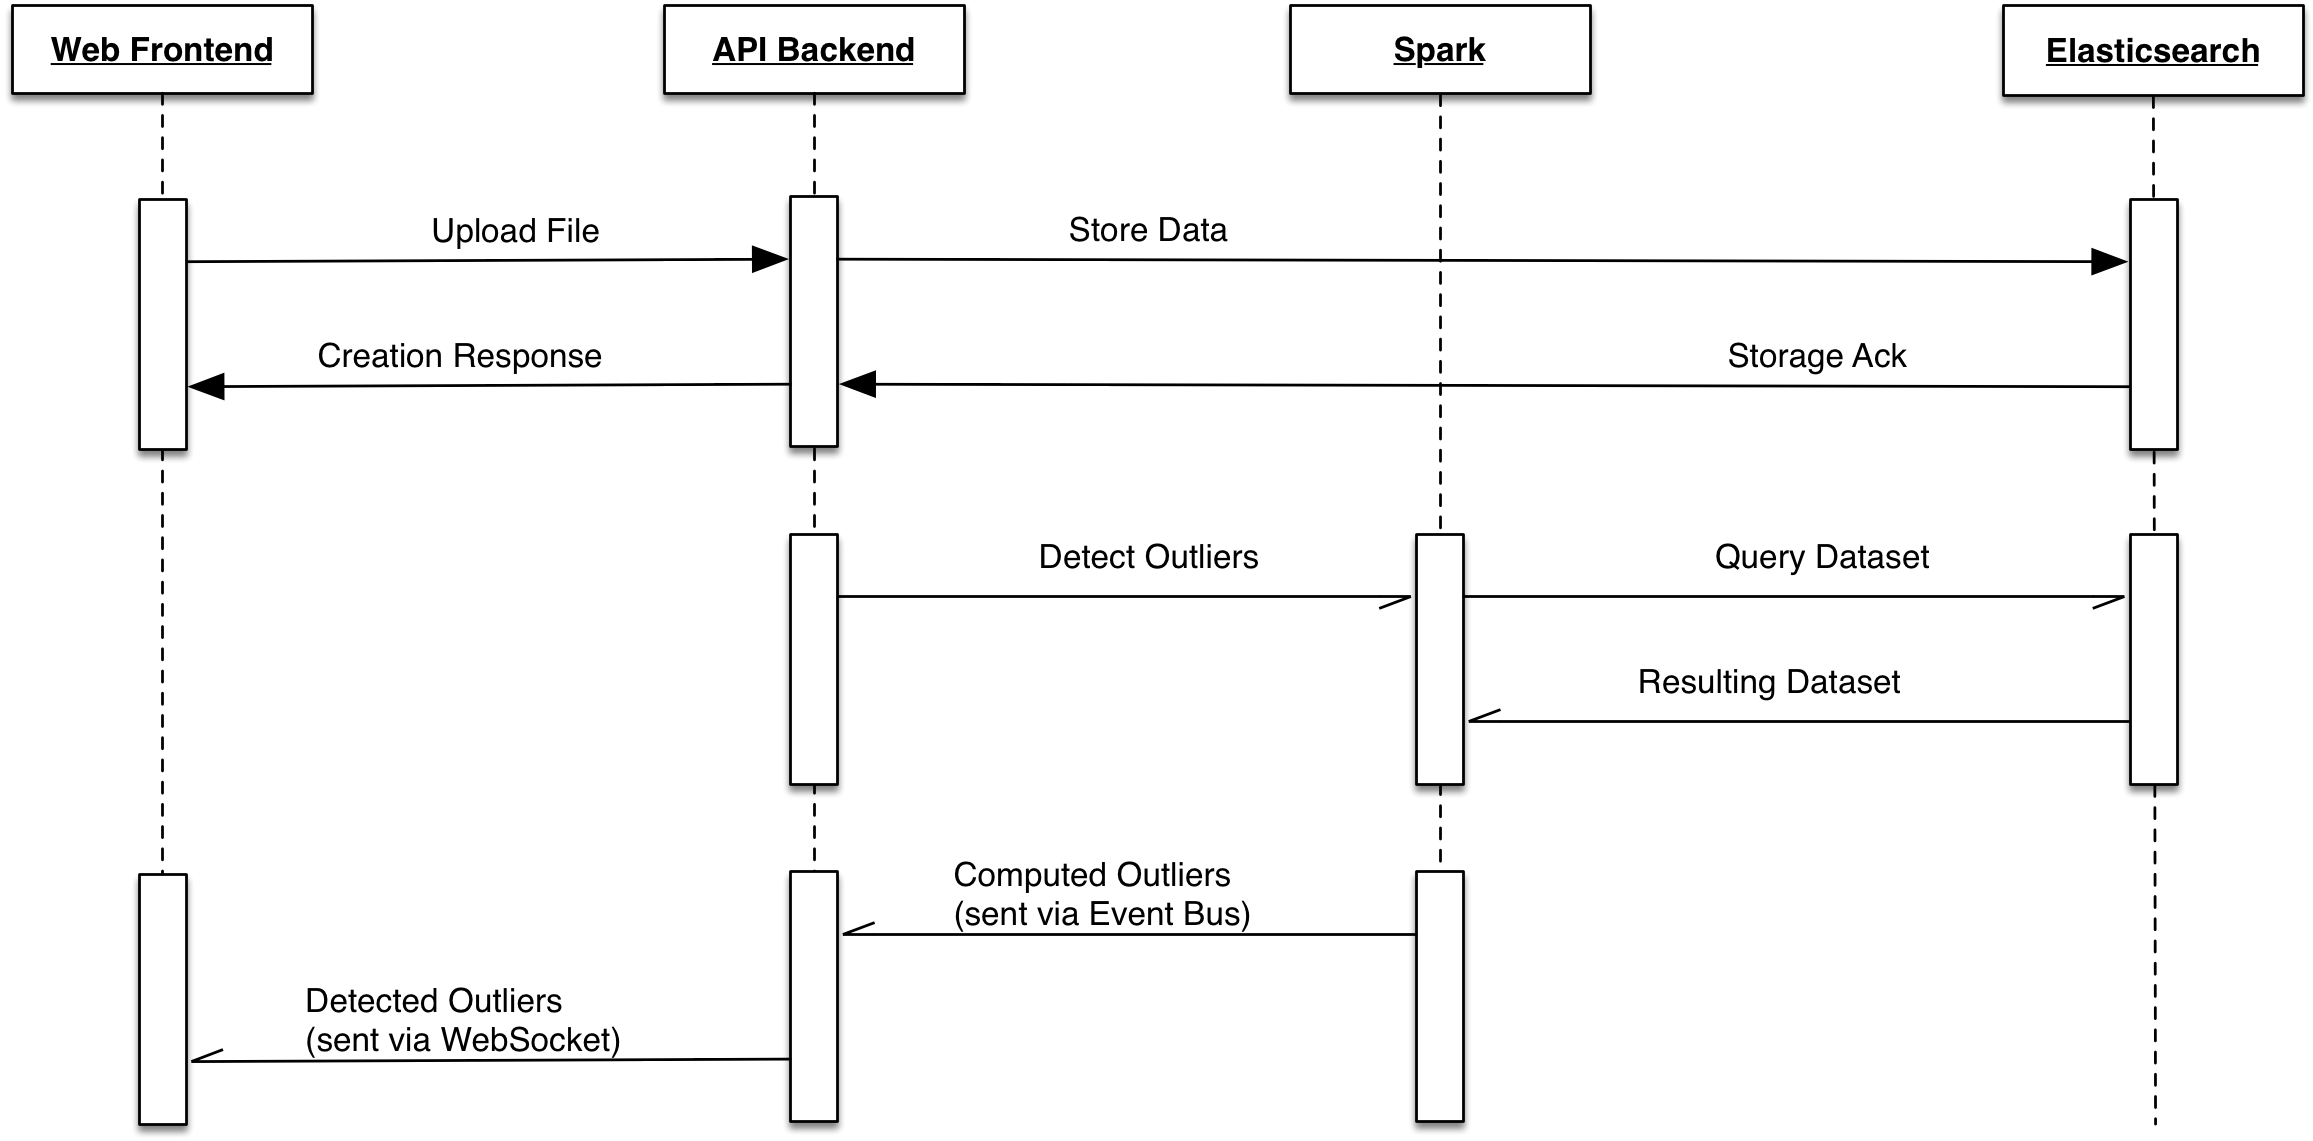
\includegraphics[width=1.025\textwidth]{figures/implementation/outlier-detection-sequence}
  \caption{Sequence diagram showing the general outlier detection on upload flow.}
  \label{fig:outlier-detection-sequence}
\end{figure}

\newpage


\subsection{Workflows and Screens}

In this section, workflows plus related screens of the implemented prototype\index{prototype} are described and explained.
Moreover, special emphasis is laid upon the reasoning behind the chosen path of the solution.


\subsubsection{Upload and Outlier Detection}

Initially, the user will want to upload some dataset to the application.
Therefore, a modal upload dialog is pretty conveniently reachable in the upper right corner of the screen.
This button is also visually especially noticeable via its peculiar coloring.
The upload dialog itself is designed\index{design} as simple as possible (see Figure~\ref{fig:screenshot-upload}).
One can either simply drag \& drop a file to it or select one via \gls{fs} dialog.
As soon as a file is selected, the upload begins and is indicating its progress via related animations.
In general, whenever data is being fetched respectively backend requests are issued, a spinning wheel effect is shown in the upper left corner of the screen.
When uploading is finished the dialog disappears and the user is free to interact with the data.

\begin{figure}[h]
  \centering
  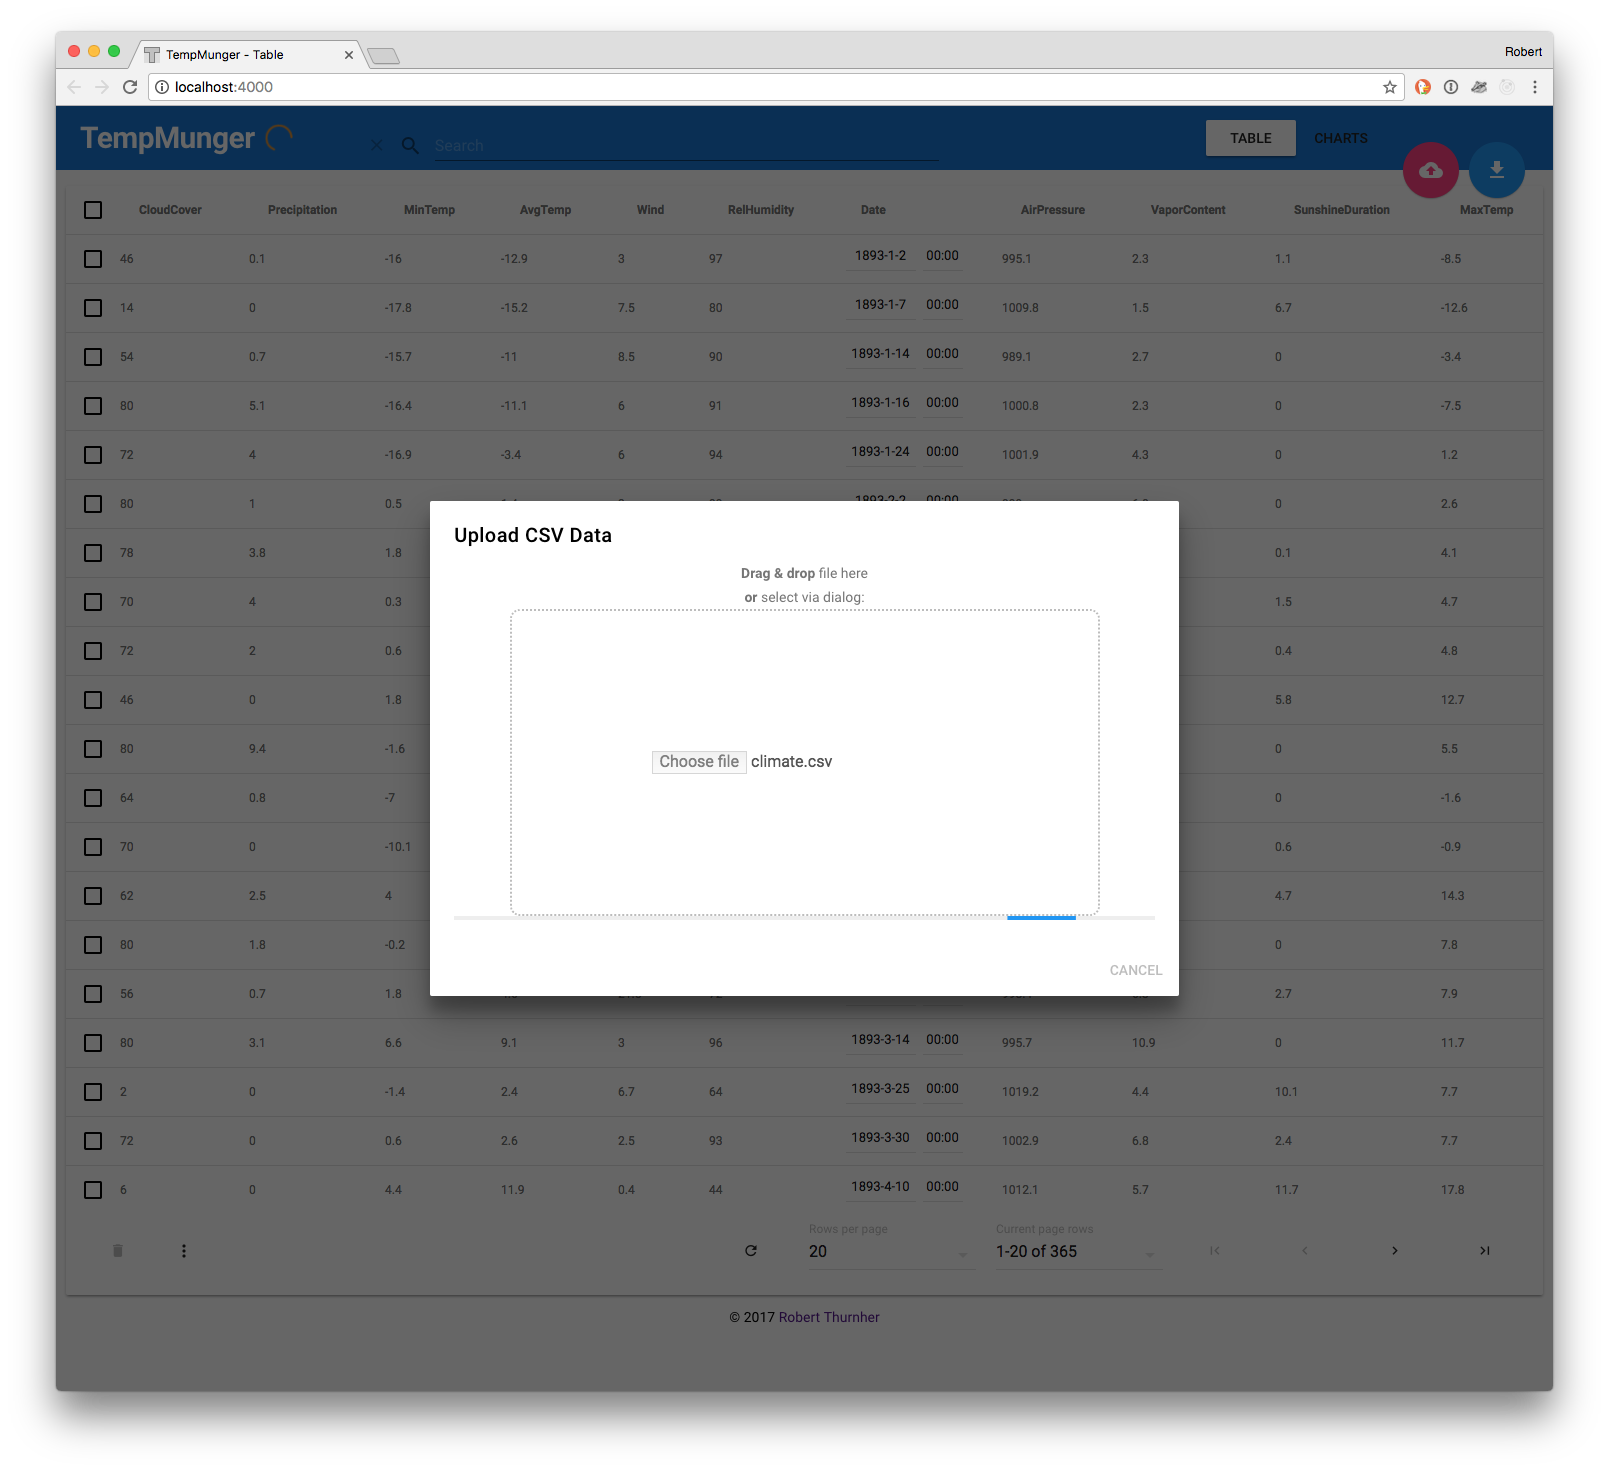
\includegraphics[width=1.0\textwidth]{figures/implementation/screenshot-upload}
  \caption{Screenshot showing upload with corresponding modal dialog and animated effects regarding progress indication.}
  \label{fig:screenshot-upload}
\end{figure}

As presented more from its technical side before, when uploading, an outlier detection mechanism is triggered.
On finished processing, the user is shown an according notification.
This message is sent as desktop browser respectively system notification\footnote{\textcolor{blue}{\href{https://developer.mozilla.org/en-US/docs/Web/API/Notifications_API}{developer.mozilla.org/en-US/docs/Web/API/Notifications\_API}}} (see Figure~\ref{fig:screenshot-notification}) as well as within the application itself as some sort of flashing notification from the bottom of the screen (see Figure~\ref{fig:screenshot-table-editor}).
The former stay around while the latter disappear.

When clicking a notification, an action is triggered filtering all dataset entries down to the potentially outlying ones.
The user may then proceed to act upon accordingly, having the potential outliers ready in sight and at her/his fingertips.
Presence of this filter is indicated via a chip-like control at the top of the screen (see Figure~\ref{fig:screenshot-search+filtering}).
It can be removed simply by clicking.

\begin{figure}[h]
  \centering
  
\includegraphics[width=0.66\textwidth]{figures/implementation/screenshot-notification}
  \caption{Screenshot showing desktop browser respectively system notification for interactive suggestive outlier detection indication.}
  \label{fig:screenshot-notification}
\end{figure}

\subsubsection{Table Editor}

A central component of the \gls{ui} is the table editor view page (see Figure~\ref{fig:screenshot-table-editor}).

There the user can directly manipulate the data at hand via editing corresponding cells.
Pagination controls at the bottom of the page allow for convenient paging through the data.
Page size can be adjusted as well as a particular page selected via related dropdowns.
Multi-row deletion is supported via selection checkboxes at the left side of the table.
It is possible to select rows one-by-one or (de)select all at once.
The connected deletion button is located at the bottom left of the table.

\subsubsection{Date/Time Picker}

Date and time picker \gls{ui} controls are used whenever an editable input field contains time-oriented\index{time-oriented} data.

The date picker allows the user to choose a date in an interactive way with the metaphor of a more traditional calendar (see Figure~\ref{fig:screenshot-date-picker}).
Whereas the time picker uses the metaphor of an analog clock for choosing a time value (see Figure~\ref{fig:screenshot-time-picker}).

\begin{figure}[h]
  \centering
  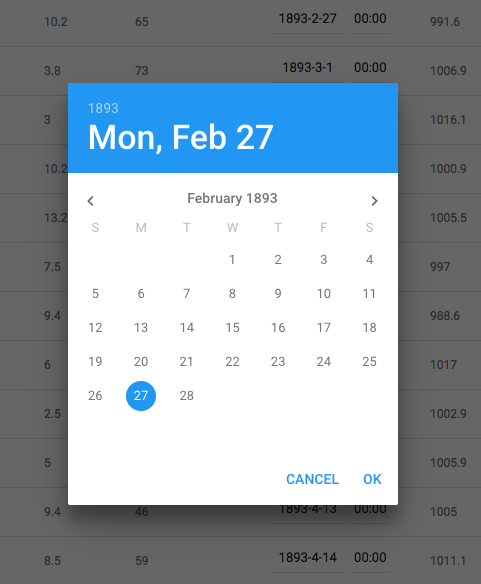
\includegraphics[width=0.525\textwidth]{figures/implementation/screenshot-date-picker}
  \caption{Screenshot showing exemplary modal date picker control with its calendar interaction metaphor.}
  \label{fig:screenshot-date-picker}
\end{figure}

\begin{figure}[h]
  \centering
  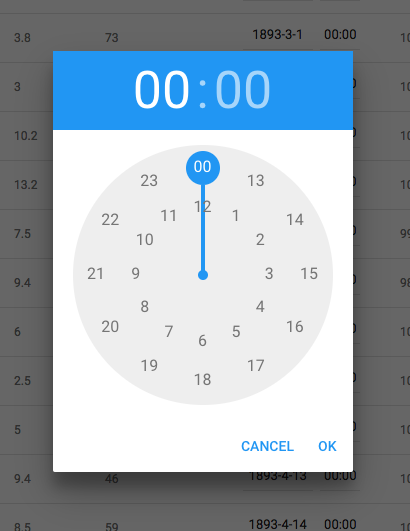
\includegraphics[width=0.525\textwidth]{figures/implementation/screenshot-time-picker}
  \caption{Screenshot showing exemplary modal time picker control with its clock interaction metaphor.}
  \label{fig:screenshot-time-picker}
\end{figure}

Both of these controls are commonly used throughout the application and normally in cooperation.
For instance, the table editor employs the controls for editing temporal column row values.

\subsubsection{Search and Filtering}

There are various ways in which filtering, slicing, and dicing the dataset is supported:

\begin{itemize}
  \item First of all, a search box is placed quite prominently at the top of the screen.
This enables the user to filter data down via full-text search.
  \item Additionally, as mentioned above, multiple rows can be selected.
Filter presence is indicated via aforementioned chip-like control.
The filter affects displayed data in the charts view page as well.
  \item Rows can be sorted by column values in ascending or descending order.
For this a simple click on the respective column header suffices.
  \item Furthermore, on the table view page there is a pagination available, see above.
\end{itemize}

All of these filtering options are working together correspondingly (see Figure~\ref{fig:screenshot-search+filtering}).

\subsubsection{Missing Values Cleanup}

It is possible to clean up missing and/or erroneous values via a modal dialog overlay (see Figure~\ref{fig:screenshot-missing-values}).
Missing respectively erroneous in this context means that the values were not able to be parsed as temporal.
The dialog can be accessed from the table editor view page at the bottom left via menu.
Its menu option is only available when the currently loaded dataset contains at least one time-oriented\index{time-oriented} data field.

On the modal dialog there is a dropdown to select one of the available temporal fields.
Below it there is a horizontal multi-bar chart consisting of two bars.
One of them represents all rows, and the other, missing values.
The former are colored in a neutral gray, while the latter are colored orange.
Consequently, a visual emphasis on the missing values is established.
The bars can be displayed grouped or stacked to get a better feel of the quantities at hand.
Below the chart there is a date and a time picker control for choosing a target value to fill the missing values with.
It is originally set to the average value of all values of the respective field (excluding missing ones).
At the bottom of the dialog there are action buttons to either apply the fill operation as described or to delete all rows with missing values.

\begin{figure}[h]
  \centering
  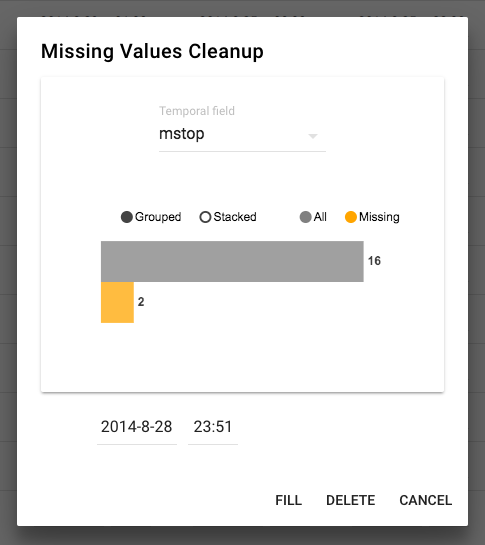
\includegraphics[width=0.7\textwidth]{figures/implementation/screenshot-missing-values}
  \caption{Screenshot showing missing values cleanup modal dialog overlay with charts.}
  \label{fig:screenshot-missing-values}
\end{figure}

\subsubsection{Temporal Normalization}

There are, basically, two types of temporal normalization operations supported by the prototype\index{prototype} -- this is not representing normalization in the strictest mathematical sense:

\begin{enumerate}
  \item Transform\index{transformation} all values within a certain timespan or at a certain point in time to a specified date/time
  \item Transform\index{transformation} all values within a certain interval, effectively ``moving'' them in time
\end{enumerate}

The former can be accessed either by clicking on a calendar heatmap or a distribution chart bar item on the charts view page (see Figure~\ref{fig:screenshot-charts-dialog}).
It is generally showing the selected timespan or point in time and enabling the user to set a target value via date and time picker controls for transforming\index{transformation} all affected values to.
Alternatively, the user can choose to delete all rows within the temporal selection.

\begin{figure}[h]
  \centering
  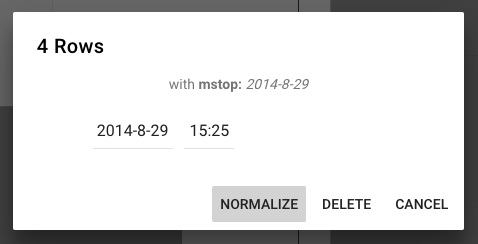
\includegraphics[width=0.66\textwidth]{figures/implementation/screenshot-charts-dialog}
  \caption{Screenshot showing charts page modal dialog on bar or heatmap item click.}
  \label{fig:screenshot-charts-dialog}
\end{figure}

The latter is accessible via a dedicated menu item at the bottom of the table editor view page, next to the one for missing values cleanup (see Figure~\ref{fig:screenshot-normalization}).
There the user can select a temporal field and interval, offering year or month.
When month is chosen at max. 10 bars in a chart are displayed each representing a month.
When year is chosen the bars represent years.
This is an aggregated view visualizing distribution of values with respective amounts sorted in descending order.
Again, bars are colored in a neutral gray. When selecting a bar its color changes to black, signalizing the selection. Plus, temporal input field controls show up. In the case of year interval being selected, there is a numeric text input for a target year.
In the case of month interval selection, there is additionally a dropdown with the 12 months of a year.
In addition to transforming\index{transformation} values accordingly, the user can also choose to delete selected rows instead.

\begin{figure}[h]
  \centering
  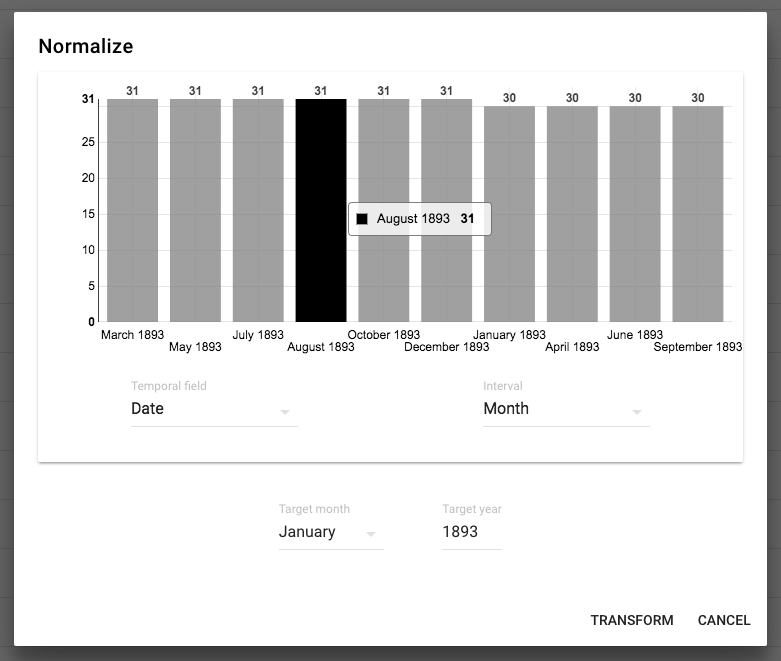
\includegraphics[width=1.0\textwidth]{figures/implementation/screenshot-normalization}
  \caption{Screenshot showing interval normalization modal dialog overlay with interactive bar charts and controls.}
  \label{fig:screenshot-normalization}
\end{figure}

\subsubsection{Table Column Merging}

It is possible to merge time-oriented\index{time-oriented} data columns via drag \& drop of table editor headers (see Figure~\ref{fig:screenshot-column-merge}).
Only columns containing temporal data are able to be drag \& dropped.
Interaction flow, generally, works as follows:

\begin{itemize}
  \item When starting to drag a header, possible drop targets (i.e., other temporal column headers) are highlighted in light yellow background color
  \item When dragging over a possible drop target, the hovered column header is highlighted in light green to signalize the drop possibility to the user
  \item When dragging over a non-temporal column header, it is highlighted in light orange color indicating that it is not a possible drop target
  \item When the user drops the dragged header on a possible target, a corresponding modal dialog overlay opens
\end{itemize}

This dialog asks the user to confirm merging columns as specified or cancel otherwise.
Merging, basically, works in the following way:

\begin{itemize}
  \item If both column values contain a temporal one, an average of these is used for the merged value
  \item If only one column value contains a temporal one, the missing one is substituted with the existing
  \item If both column values contain missing ones, an overall average of all values of the two columns is used
\end{itemize}

An alternative implementation could have given the user options to choose in a more fine-grained way.
Yet, we have found that these sensible defaults should make sense in many cases and the user can still apply further refinements of the column data after merge, if desired.
Naturally, on finished operation, the merge respectively drag source column is removed.

\begin{figure}[h]
  \centering
  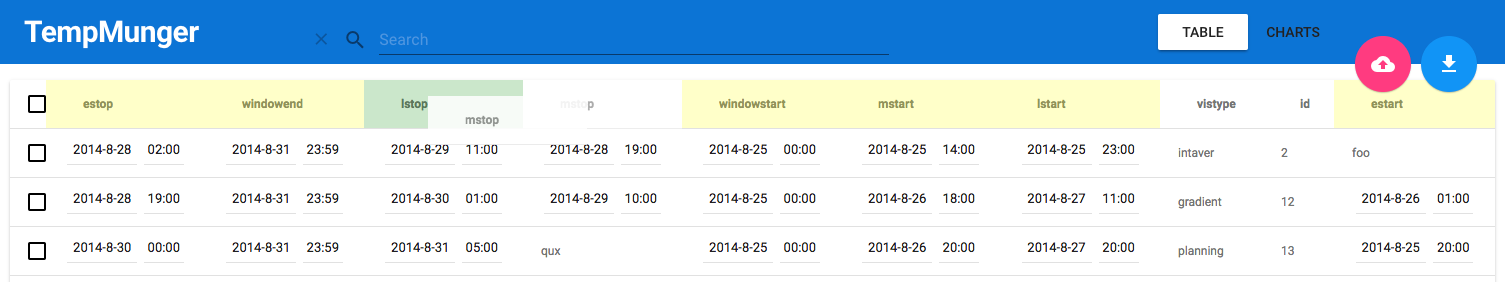
\includegraphics[width=1.0\textwidth]{figures/implementation/screenshot-column-merge}
  \caption{Screenshot showing table column merging via drag \& drop interaction.}
  \label{fig:screenshot-column-merge}
\end{figure}

\subsubsection{Charts Page}

The central \gls{ui} component regarding charts is kind of a dashboard page (see Figure~\ref{fig:screenshot-charts-page}).

When there are time-oriented\index{time-oriented} fields present in the respective dataset, it is headed by an interactive calendar heatmap visualization. It gives the user the opportunity to understand the temporal dimension of the data as well as transforming\index{transformation} it. Temporal fields can be selected via dropdown.

In any case and below there are two distribution bar charts next to each other.
These charts enable the user to get a grasp of the present data, plus transforming\index{transformation} it, too.
Again, fields can be selected via dropdown.

\subsubsection{Calendar Heatmap}

The calendar heatmap visualization, generally, allows four temporal scales \\(see Figure~\ref{fig:screenshot-calendar-heatmap}):

\begin{enumerate}
  \item Year
  \item Month (default)
  \item Week
  \item Day
\end{enumerate}

\begin{figure}[h]
  \centering
  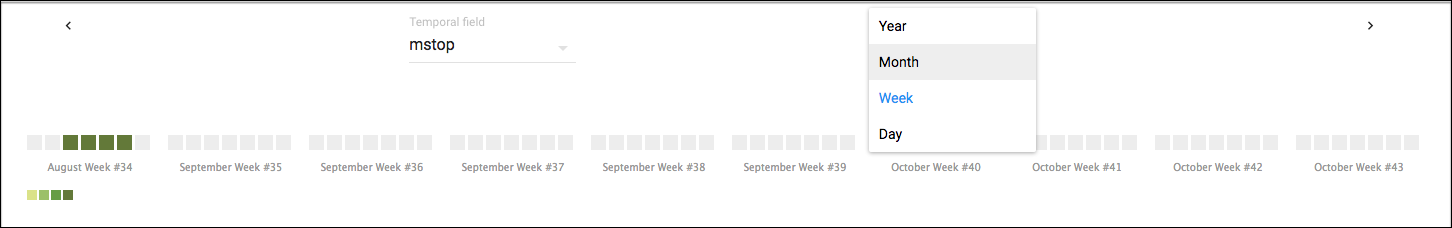
\includegraphics[width=1.0\textwidth]{figures/implementation/screenshot-calendar-heatmap}
  \caption{Screenshot showing calendar heatmap visualization with interactive controls.}
  \label{fig:screenshot-calendar-heatmap}
\end{figure}

Depending on the chosen scale the calendar view adjusts accordingly.
So, for instance, in the case of month scale, it is showing days of each month as boxes.
Furthermore, a color scale from gray via light to dark green indicates the amount of dataset entries associated with a certain temporal value represented by such a calendar item box.
On click of an item box, a modal dialog is shown, giving the user transform\index{transformation} options.

\subsubsection{Distribution Charts}

The two distribution bar charts can be seen as some sort of histogram visualizations, showing top aggregations.
They are mainly pointed at enabling the user to understand general data distribution qualities of the dataset at hand.
Plus, making it possible to easily compare these (see Figure~\ref{fig:screenshot-bar-charts}).
Again, clicking a bar opens a modal dialog for further interactive transformation\index{transformation} operations, like deletion or time-oriented\index{time-oriented} normalization.

\subsubsection{Export}

At the end of the day, the user wants to export the wrangled\index{wrangle} data.
Therefore, a button is quite prominently placed in the upper right corner of the application.
When there is no time-oriented\index{time-oriented} data included, a button click simply initiates a \textsc{CSV} file export download.
Otherwise, a modal dialog overlay is presented first.
This dialog lets the user choose a format to apply to all time-oriented\index{time-oriented} data of the to be exported dataset (see Figure~\ref{fig:screenshot-export-dialog}).

\begin{figure}[h]
  \centering
  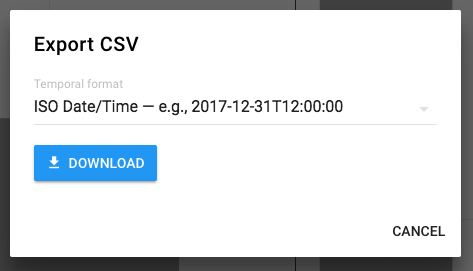
\includegraphics[width=0.66\textwidth]{figures/implementation/screenshot-export-dialog}
  \caption{Screenshot showing modal export dialog with temporal format dropdown.}
  \label{fig:screenshot-export-dialog}
\end{figure}

Three options are implemented and, consequently, available:

\begin{enumerate}
  \item \textsc{ISO}\footnote{\textcolor{blue}{\href{http://www.iso.org/iso/iso8601}{www.iso.org/iso/iso8601}}} date/time (e.g., \emph{2017-12-31T12:00:00})
  \item \textsc{ISO} date (e.g., \emph{2017-12-31})
  \item Epoch millis (e.g., \emph{1485037113334})
\end{enumerate}

Since all time-oriented\index{time-oriented} data is formatted on export in a unified way as well as uniformly stored in \gls{utc}/\gls{gmt} timezone on upload, there is no need to support formatting during previous editing and transformation\index{transformation} interactions.

\begin{sidewaysfigure}[h]
  \centering
  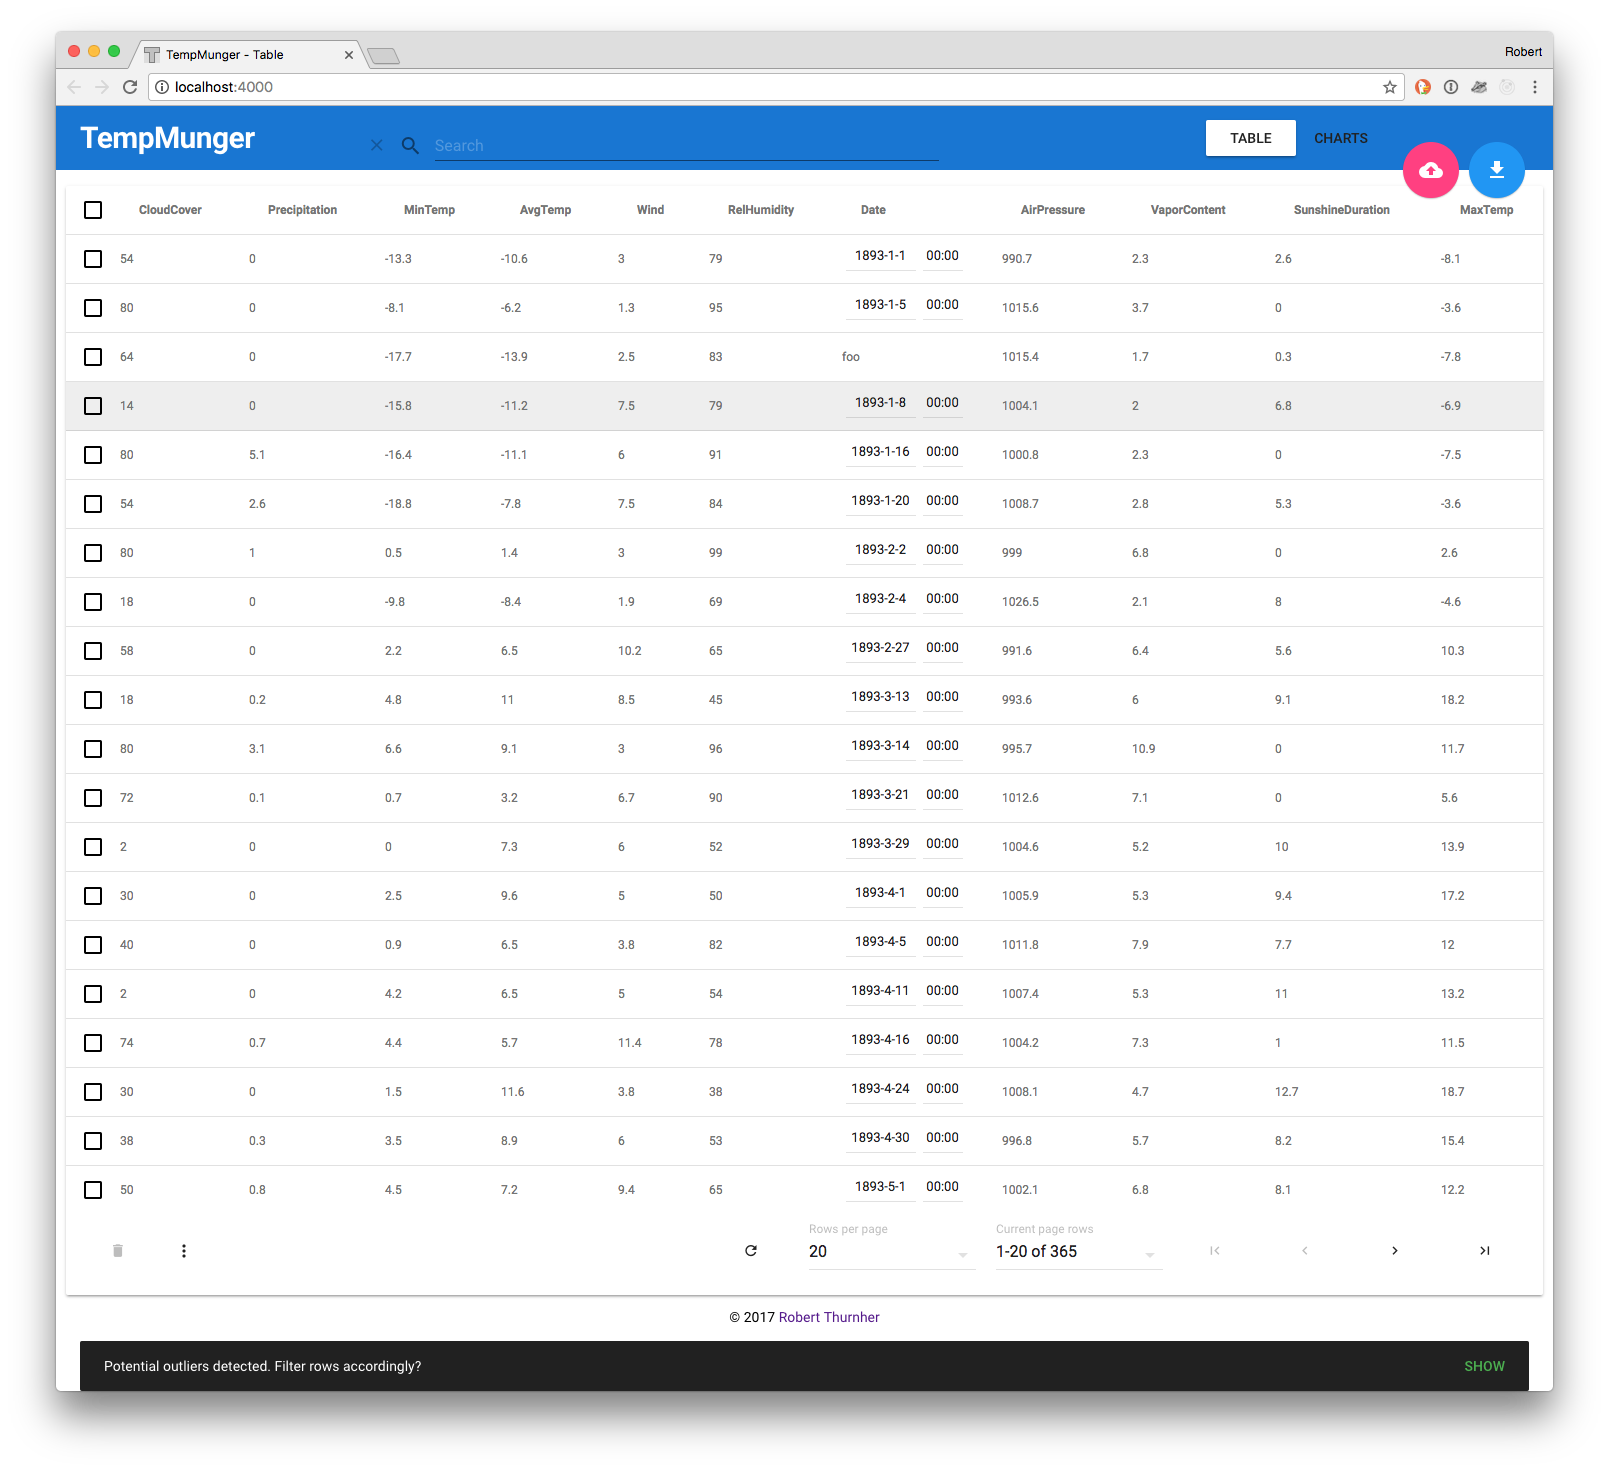
\includegraphics[width=0.9\textwidth]{figures/implementation/screenshot-table-editor}
  \caption{Screenshot showing table editor respectively main page including outlier detection info alert.}
  \label{fig:screenshot-table-editor}
\end{sidewaysfigure}

\begin{sidewaysfigure}[h]
  \centering
  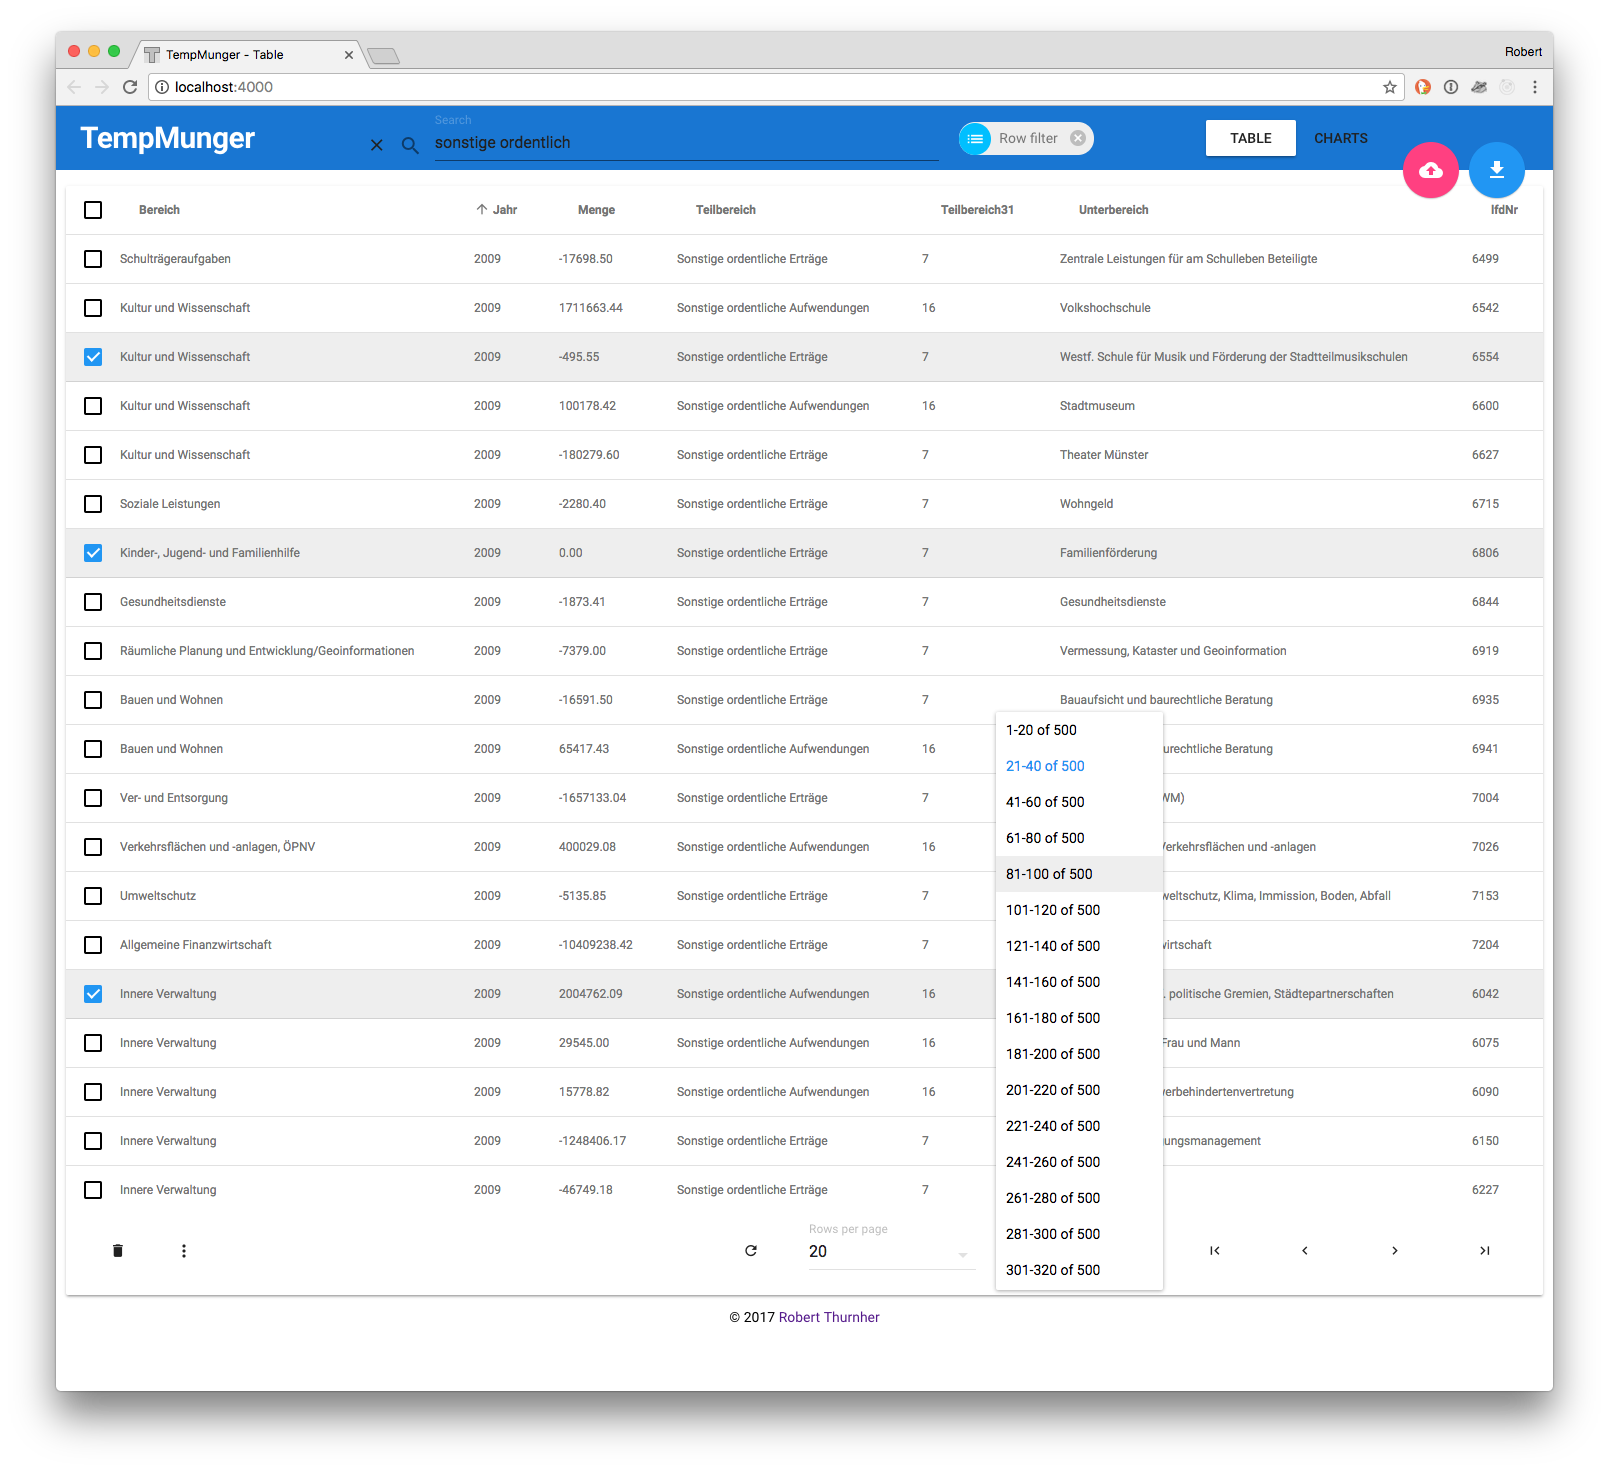
\includegraphics[width=0.9\textwidth]{figures/implementation/screenshot-search+filtering}
  \caption{Screenshot showing various navigational, search, and filtering options with table editor view.}
  \label{fig:screenshot-search+filtering}
\end{sidewaysfigure}

\begin{figure}[h]
  \centering
  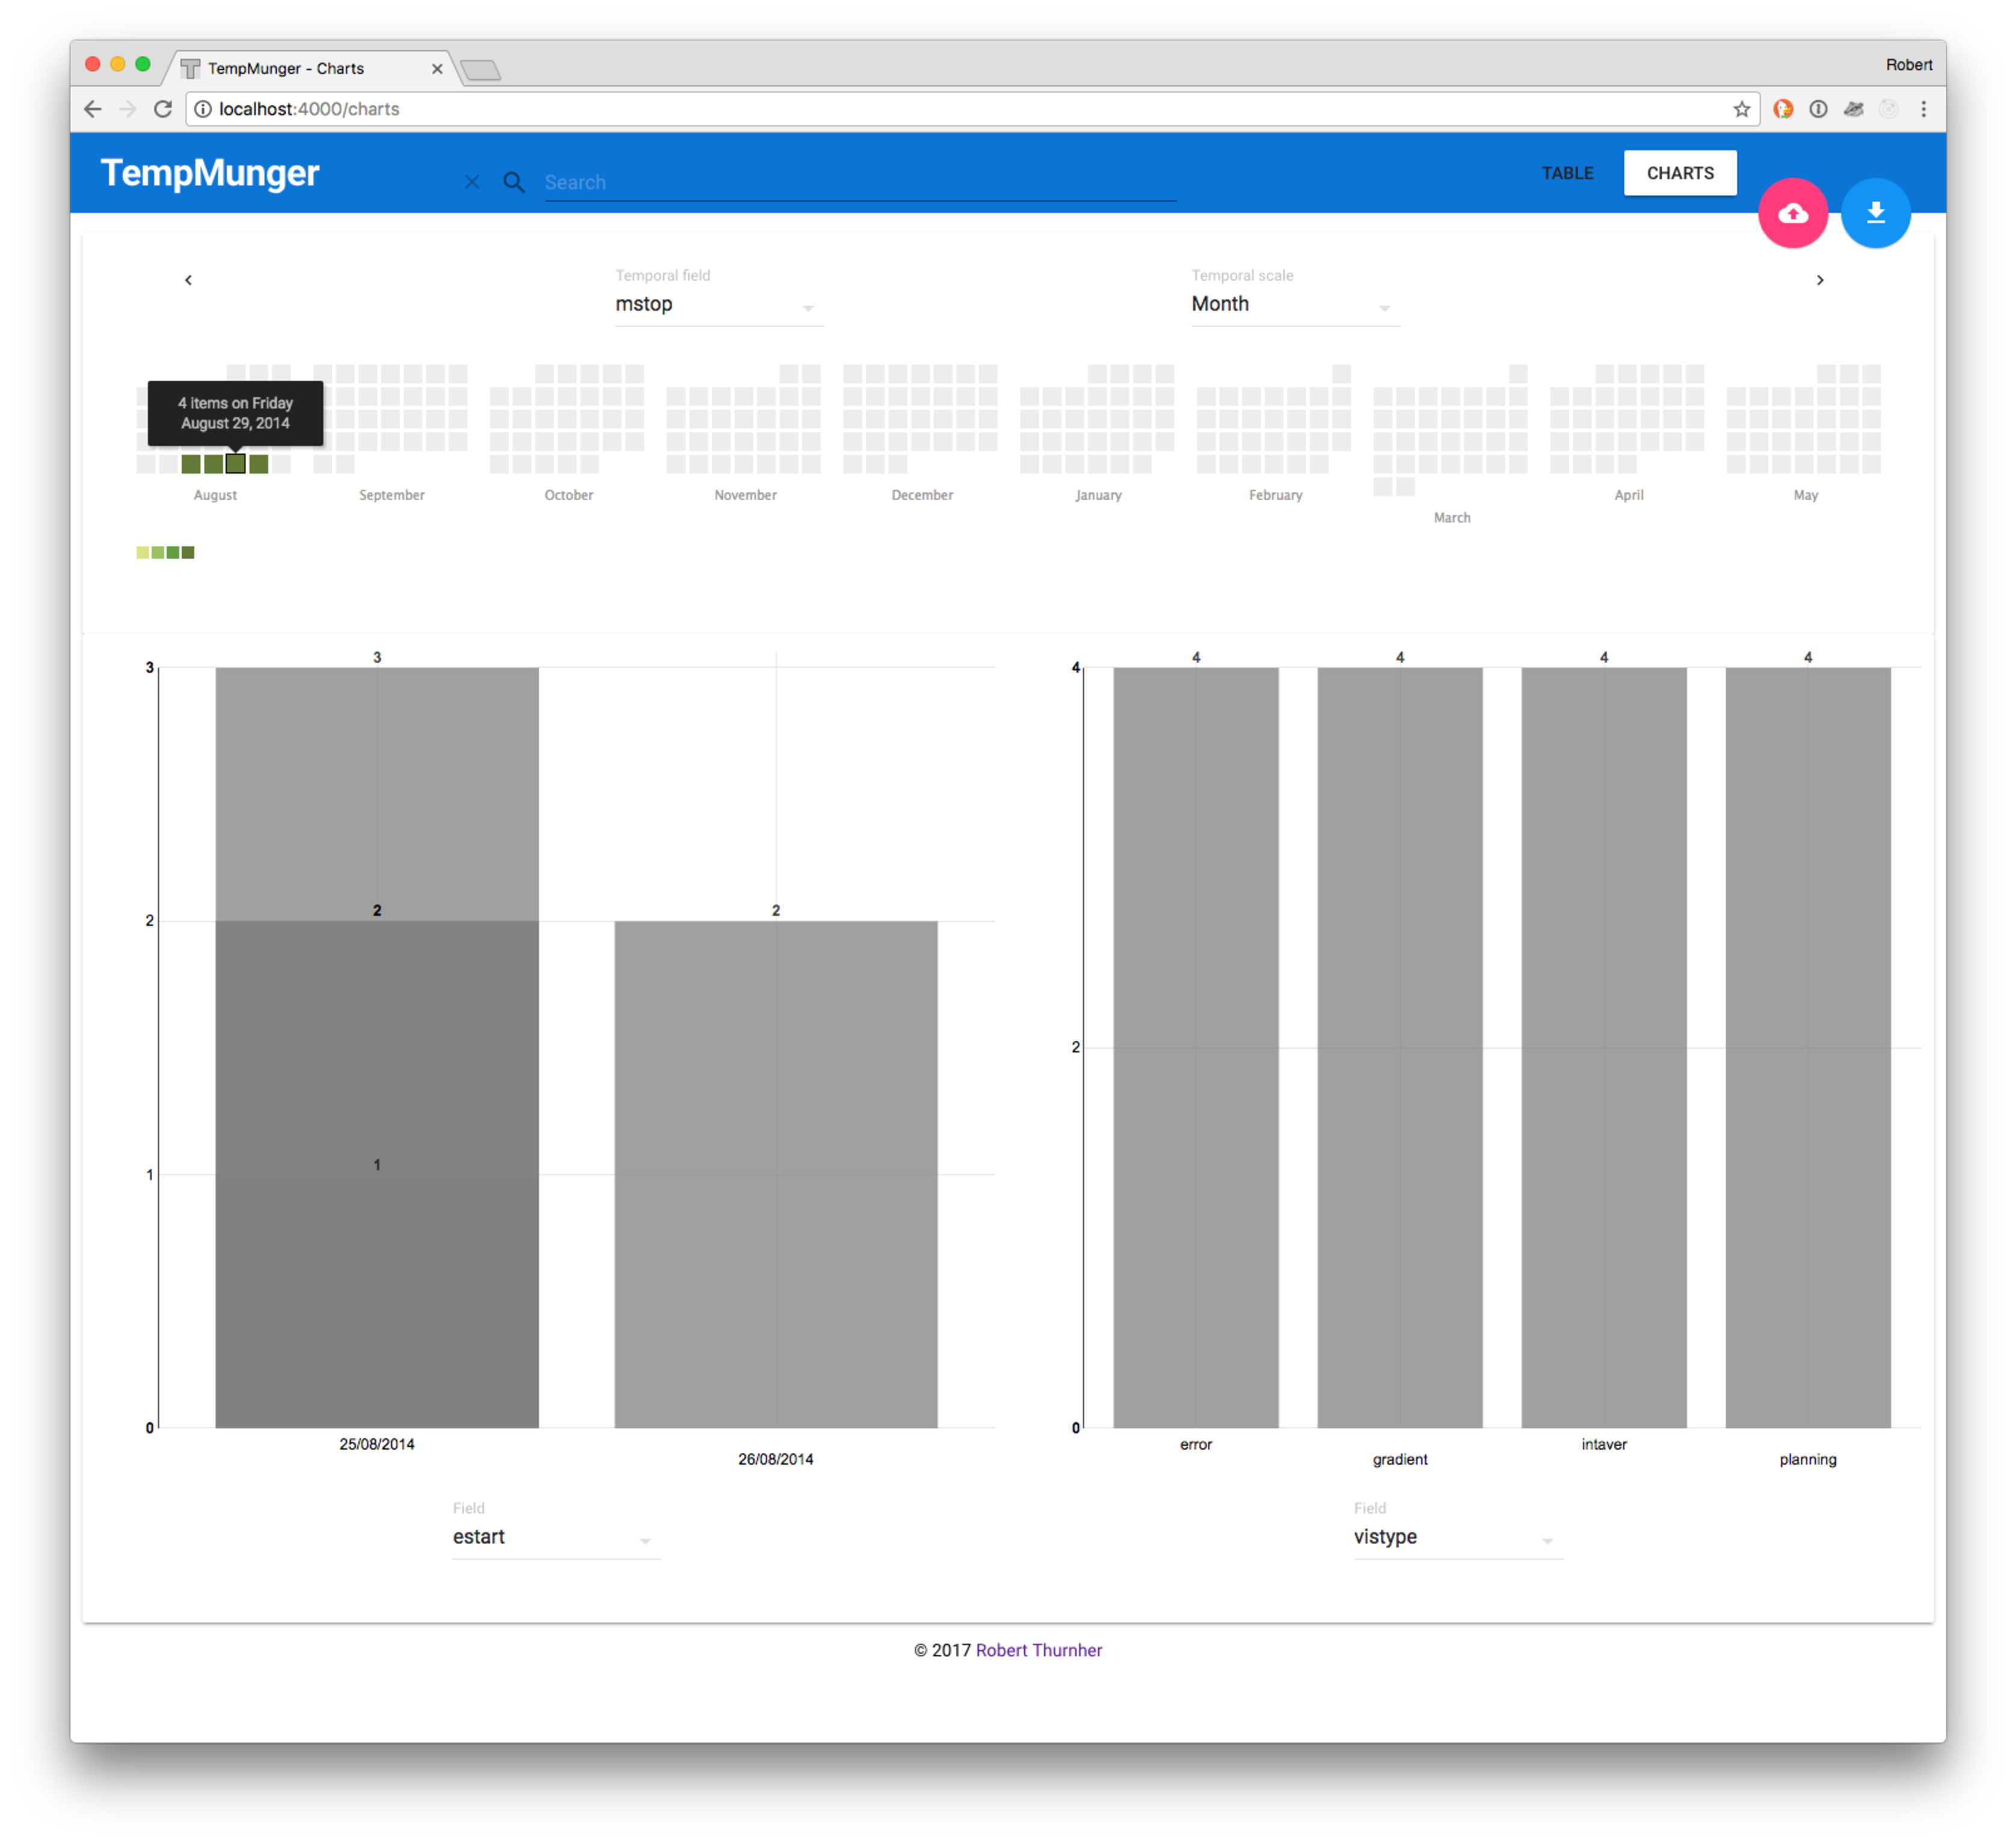
\includegraphics[width=0.9\textwidth]{figures/implementation/screenshot-charts-page}
  \caption{Screenshot of charts page with calendar heatmap, offering visual overview.}
  \label{fig:screenshot-charts-page}
\end{figure}

\begin{figure}[h]
  \centering
  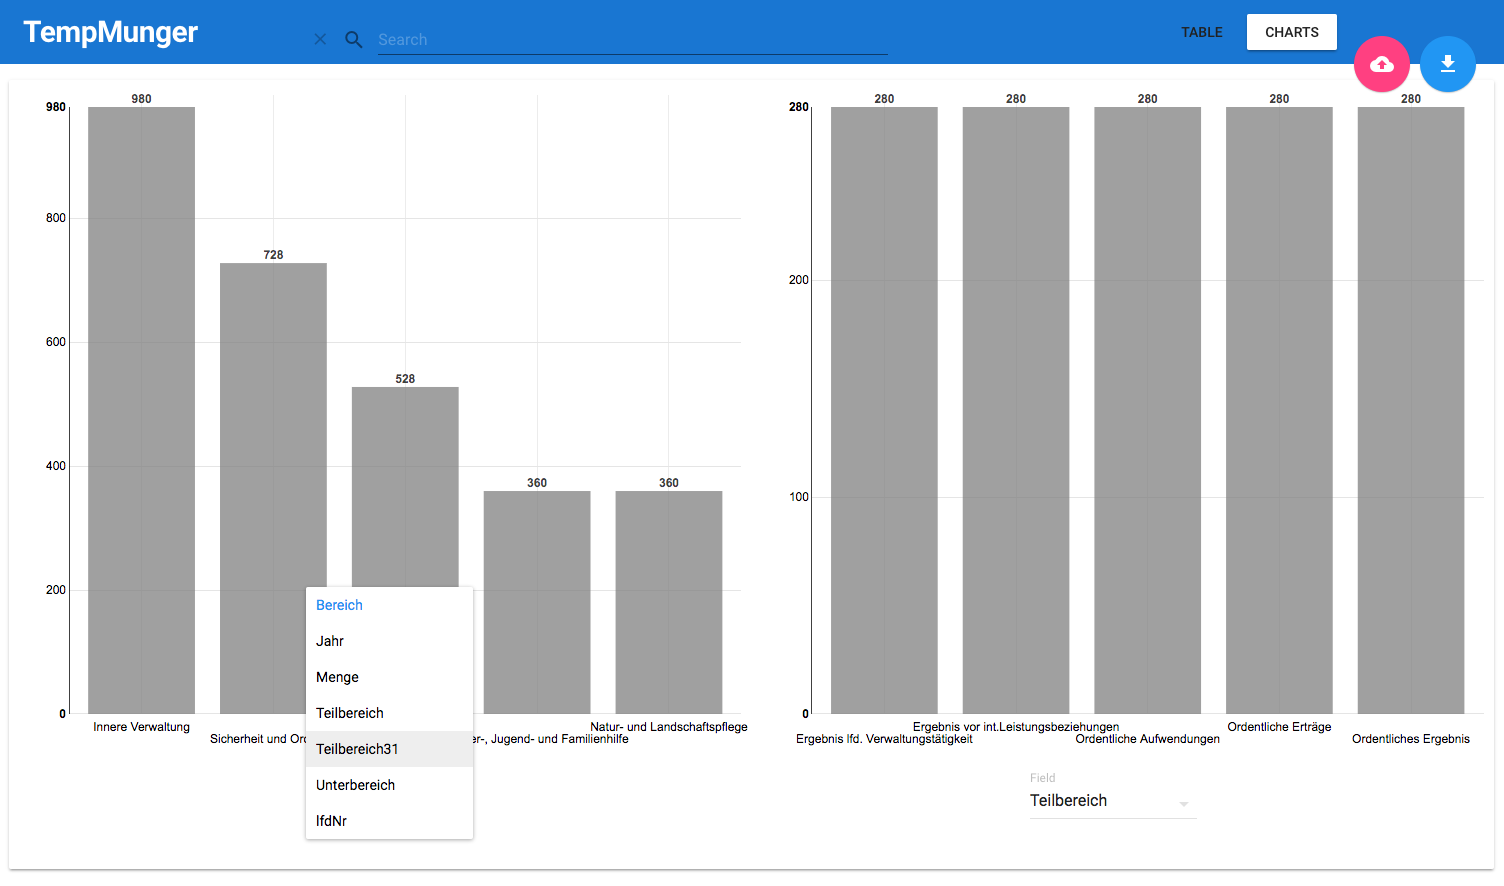
\includegraphics[width=0.777\textwidth]{figures/implementation/screenshot-bar-charts}
  \caption{Screenshot showing distribution bar charts with their dropdown controls.}
  \label{fig:screenshot-bar-charts}
\end{figure}


\section{Qualitative Evaluation} \label{sec:qualitative-evaluation}

Eventually, the results had to be evaluated.
For that matter, we have employed two well-known approaches\index{approach} and tools from the domain of usability engineering.
Both of which are introduced and extensively explained in \cite{Nielsen1993}:

\begin{enumerate}
  \item \textbf{Heuristic evaluation}
  \item \textbf{User/usability tests}
\end{enumerate}

The former basically means that an application and especially its \gls{ui} is being evaluated by a group of usability experts, step by step examining the to be evaluated system.
According to Holzinger~\cite{Holzinger2005} three to five usability experts are sufficient for this type of evaluation.
Therefore, we have conducted an heuristic evaluation with three experts.
Each of the experts should, further, evaluate independently from the others.
The evaluation is generally based on heuristics related to usability.
The classic ones as described by Nielsen~\cite{Nielsen1993} are:

\begin{itemize}
  \item \emph{Visibility of system status}
  \item \emph{Match between system and the real world}
  \item \emph{User control and freedom}
  \item \emph{Consistency and standards}
  \item \emph{Error prevention}
  \item \emph{Recognition rather than recall}
  \item \emph{Flexibility and efficiency of use}
  \item \emph{Aesthetic and minimalist design\index{design}}
  \item \emph{Help users recognize, diagnose, and recover from errors}
  \item \emph{Help and documentation}
\end{itemize}

Forsell and Johansson~\cite{Forsell2010} identified heuristic sets which are especially useful when dealing with applications in the realm of \gls{infovis}.
Therefore, we are adding the following:

\begin{itemize}
  \item \emph{Information coding}
  \item \emph{Spatial organization}
  \item \emph{Remove the extraneous}
\end{itemize}

For the evaluation itself each expert is asked to perform a given set of tasks.
Before that, a session going through the application and \gls{ui} in general is conducted.
An observer is present at the evaluation, who is familiar with the application and can be asked related questions.
The respective evaluator should note all issues.
At the end, found results are gathered and summarized.

These are the tasks we have established for our evaluation:

\begin{enumerate}
  \item Upload a dataset using a given \textsc{CSV} file
  \item Edit time-oriented\index{time-oriented} data via table editor
  \item Find potential outliers in the given dataset
  \item Identify missing respectively erroneous values
  \item Fill these with actual temporal values and/or delete their entries
  \item Normalize all entries in a certain month, moving them to another one
  \item Move all entries on a specific day to another point in time
  \item Delete all entries within a certain timespan or on a certain date
  \item Merge time-oriented\index{time-oriented} data columns on the table editor view page
  \item Export data as \textsc{CSV}, choosing a format for time-oriented\index{time-oriented} values
\end{enumerate}

User or usability tests, on the other hand, are usually performed in some sort of lab environment.
That is, users are given tasks to execute for reaching certain goals with the application and are being observed while doing so.
Typically, the test participants should be actually potential users.
We have performed such tests with two users, thus, in addition to the previous heuristic evaluation which we have conducted with three different usability and visualization experts.
The users of the user/usability tests were given the same tasks to perform as the experts from heuristic evaluation before.
Meanwhile testing and particularly afterwards they were interviewed regarding their experience, impressions, and opinions.
Finally, we have analyzed and abstracted connected findings.

The main questions all such user test participants as well as heuristic evaluation ones were asked:

\begin{enumerate}
  \item What is your overall impression?
  \item What are the strengths of TempMunger?
  \item What are the shortcomings of TempMunger?
  \item Do you believe TempMunger can be useful for you?
  \item If not, what do you think is needed to make it so?
\end{enumerate}

Combined results of the heuristic evaluation and user tests are as follows, listing found issues and linking them to their respective related, violated heuristics:

\begin{enumerate}
  \item Insufficient immediate and intuitive visual feedback regarding performed actions, e.g., on missing values cleanup ($\rightarrow$ \emph{visibility of system status})
  \item Findability of modal dialogs for missing values cleanup and interval-based normalization is suboptimal ($\rightarrow$ \emph{spatial organization})
  \item Separation of the two normalization dialogs as well as connected semantics are not intuitive and could be refined ($\rightarrow$ \emph{consistency and standards})
  \item Granularity of temporal scale is partially incomplete ($\rightarrow$ \emph{user control and freedom})
  \item Temporal scale coloring in calendar heatmap visualization is sometimes misleading ($\rightarrow$ \emph{information coding})
  \item No dedicated highlighting of concrete outlier values, for instance, via corresponding coloring ($\rightarrow$ \emph{recognition rather than recall})
  \item Outlier detection action could be made repeatable via button ($\rightarrow$ \emph{flexibility and efficiency of use})
  \item Merging operation could be made more useful by offering options and information regarding algorithm ($\rightarrow$ \emph{user control and freedom})
  \item Distribution charts for exploratory comparison on charts page could be enhanced, e.g., by adding drilling functionality ($\rightarrow$ \emph{information coding})
  \item In some places labels could be added to make controls and respective intention clearer ($\rightarrow$ \emph{remove the extraneous})
  \item Missing values cleanup dialog visualization could be refined, for instance, by making stacked charts view the default ($\rightarrow$ \emph{information coding})
  \item Calendar heatmap visualization could be enabled to make use of drag \& drop interaction ($\rightarrow$ \emph{flexibility and efficiency of use})
  \item Time-oriented\index{time-oriented} data could be displayed localized in controls and related input fields ($\rightarrow$ \emph{information coding})
  \item Multi-delete action button could be moved to the top of screen or made contextual ($\rightarrow$ \emph{user control and freedom})
  \item Large number of columns could lead to displaying glitches on the table editor view ($\rightarrow$ \emph{spatial organization})
\end{enumerate}

The heuristic category which was noted most often is \emph{information coding}, followed by \emph{user control and freedom}.
After that, \emph{spatial organization} as well as \emph{flexibility and efficiency of use} both got an equal amount of mentions.
Other categories scored only once each.
Hence, one can deduct a relative order concerning areas for possible improvements accordingly.

Generally, the approach\index{approach} and prototype\index{prototype} was perceived positively and as moving into the right direction.
In its current state it was rather seen as a nice proof of concept.
To make it a real-world applicable tool it would mainly need to be completed regarding coverage of data types, apart from its focus on time-oriented\index{time-oriented} one now.
Additionally, the currently provided set of transformation operations should be completed.
Furthermore, the present chart visualizations could be refined and including additional ones was encouraged.
Most frequently, possibly dotted, line charts were referred to in the context of time series data visualization as a potentially useful addition.
A central issue to address is scalability of the visualizations, also in regard to data granularity.

Aspects of our prototype most praised were the general visual design, the good visually interactive\index{visual-interactive} overview offered with charting aid, and smoothness regarding \gls{ux}.
On the other hand, usability was also one of the most controversially discussed topics as it is by its nature a highly subjective and opinionated one.
Moreover, an area for future work identified to be desirable would be to provide more transformation\index{transformation} suggestions interactively, in a proactive way.
Also, additional focus could be laid on further increasing interactive data filtering and drilling capabilities.
An interesting idea mentioned was that it could also be useful to some users being able to export visualizations in addition to the raw \textsc{CSV} data which is currently downloadable.
Finally, a feedback given by one of the test participants, which we especially appreciate, was \emph{``it does what it's supposed to do''}.

Regarding our interview questions more concretely and in detail:
answers to the first question connected to overall impression can be summarized as TempMunger being seen as a nice tool for the use case of working with time-oriented data visual-interactively\index{visual-interactive}.
Concerning strengths, most commonly pleasantness of general design, \gls{ux}, and quality of present visualizations were mentioned.
The interactive calendar heatmap as well as histogram-like bar chart visualizations were mostly seen as basically fitting for their purpose of conveniently visualizing data distribution focusing on time-oriented aspects and, therefore, useful.
Weaknesses were mainly identified to be related to lack of completeness of supported transformation operations and visualizations.
Thus, mainly coverage of varied specificity was found to have to be completed in order to make TempMunger a really versatile tool, outgrowing being merely a research prototype.

Further discussion of open issues and future work can be found in the conclusion sections following this one.



%%%%%%%%%%%%%%%%%%%%%%%%%%%%%%%%%%%%%%%%%
\chapter{Critical Reflection}
\label{ch:reflection}
%%%%%%%%%%%%%%%%%%%%%%%%%%%%%%%%%%%%%%%%%

It is time to reflect on our solution and its results.

\section{Comparison with Related Work}

Therefore, we first conduct a comparison with related work.

Our aim with \emph{\textbf{TempMunger}} was to extend mainly the approaches\index{approach} from \emph{DataWrangler} and \emph{OpenRefine}, adding our ideas for improved \gls{ux} and focusing on time-oriented\index{time-oriented} data support, specifically.

Generally, we believe that we did reach these goals.
TempMunger supports wrangling\index{wrangle} time-oriented\index{time-oriented} datasets, both with the traditional spreadsheet-like \gls{ui} as well as special, visually interactive charting aids.
Evaluation has proven the prototypically\index{prototype} implemented approach\index{approach} to be overall useful.
Consequently, it can be seen as an advance in the field, at least to some extent.
Table~\ref{tab:reflective-comparison} offers a reflective comparison overview.

Nevertheless, there are some open issues which are being addressed in the next section.

\begin{table}
  \centering
  \begin{tabular}{cccccc}
    \toprule
                      & \emph{DataWrangler}  & \emph{OpenRefine}  & \emph{Timelion}  & \emph{Jupyter}  & \emph{\textbf{TempMunger}}  \\
    \midrule
    Time-Oriented     & No                   & Yes                & Focus                  & Supported               & Focus      \\
    Charting          & Little               & Some               & Extensive              & Extensive               & Focus      \\
    Approach          & Spreadsheet          & Spreadsheet        & \gls{cli} + \gls{dsl}  & \gls{cli} + \gls{repl}  & Dashboard  \\
    \bottomrule
  \end{tabular}
  \caption{Reflective comparison of our solution with related work.}
  \label{tab:reflective-comparison}
\end{table}

\section{Discussion of Open Issues}

So, some issues were found during evaluation which can be subsumed as follows:

\begin{itemize}
  \item The usage and behavior of the software is not always intuitive
  \item Immediate visual feedback of system state is partially lacking
  \item Sometimes possible actions are not completely clear to the user
  \item Generally, usability can be improved in some parts of the prototype\index{prototype}
  \item Moreover, interactive chart visualizations can be further augmented
  \item Scalability of visualizations should be addressed more
  \item The supported transformation operations could be enhanced
  \item Some aspects are either incomplete or could, at least, be refined
\end{itemize}

More detailed information concerning evaluation design\index{design}, process, and tests revealing these issues can be found in the corresponding Section~\ref{sec:qualitative-evaluation}.

As mentioned above, evaluation has proven the approach\index{approach} to be overall useful, though.
Furthermore, feedback regarding and inspiration for future work has been given while conducting qualitative evaluation of the approach\index{approach} and implemented prototype\index{prototype}.
To sum it up, it appears our achieved results are, all in all, heading towards the right direction.


\section{Requirements Fulfillment}

With our approach\index{approach} and prototype\index{prototype} TempMunger we think to, in general, have fulfilled the requirements as derived and listed in Section~\ref{sec:requirements-list}.

That is, it is capable of loading and working with diverse datasets (\textbf{R1}).
This is being achieved via easily uploading arbitrary \textsc{CSV} data files.
Moreover, it has proven to be, generally, intuitive for casual users (\textbf{R2}), while offering some shortcuts for rather power users (\textbf{R3}).
Focus is indeed on visual-interactive\index{visual-interactive} charting aid (\textbf{R4}) centering on applying time-oriented\index{time-oriented} data transformations\index{transformation} (\textbf{R5}).
There are numerous interactive chart visualizations provided for this purpose.
A visual overview of datasets containing time-oriented\index{time-oriented} data is offered (\textbf{R6}).
For instance, a special, interactive calendar heatmap visualization is available.
We have put emphasis on choosing most effective and efficient visualizations (\textbf{R7}).
Therefore, we have focused on employing different kinds of bar charts.
Interactively exploring datasets is convenientely possible (\textbf{R8}).
This is backed by various navigational, search, and filtering capabilities.
A more traditional tabular editor is supported as well (\textbf{R9}).
Editing time-oriented\index{time-oriented} data is enhanced with specific date and time picker controls (\textbf{R10}).
Addressing data quality issues (\textbf{R11}) like cleaning missing and erroneous values, normalizing data, and spotting outliers (\textbf{R12}) are all supported via visual-interactive\index{visual-interactive} tools and techniques.
All the identified data transformation\index{transformation} operations we have originally defined in our requirements list are supported, including merging table editor columns via easy drag \& drop interaction (\textbf{R13}).


\section{Answering the Research Questions}

Consequently, returning to our initial research questions:

\begin{enumerate}
  \item \emph{\textbf{Which data transformations\index{transformation} are best supported by analytical methods and for which transformations\index{transformation} is visual support beneficial?}}

  We have answered this with our approach\index{approach} supporting data quality cleaning, normalization, and merging operations.
  That is, we have determined these general transformations\index{transformation} to be best suited while visual support being benefecial.
  More in-depth, we are, consequentially, supporting the following transformation operations:
  \begin{itemize}
    \item Cleanup of missing and erroneous values, allowing fill and deletion
    \item Normalization of values regarding points in time and intervals
    \item Merging of time-oriented data columns, using average calculations
  \end{itemize}
  Generally, data transformations which require some sort of statistical querying and/or computation are, naturally, best supported by analytical methods.
  Moreover, whenever data has to be analyzed and/or manipulated in batches or even considering a dataset as a whole, visual support is beneficial for granting necessary overview and insights.
  The larger and diverse the dataset, the more this comes into effect.
  Fully automated techniques, on the contrary, make most sense when the transformations to apply are rather straightforward.
  Our research and design\index{design} process led to these findings, and our qualitative evaluation confirmed the results.
  \item \emph{\textbf{How do concrete \gls{datawrangling} workflow processes look like and how can these processes be supported by \gls{va} methods?}}

  We have answered this question extensively with the state of the art review and analysis\index{analysis} as well as, particularly, through the design\index{design} of our approach\index{approach} and prototype\index{prototype}.
  More concretely, such processes are oftentimes of exploratory nature.
  Thus, we are supporting them visual-interactively\index{visual-interactive}.
  Plus, especially repetitive actions, being applied to batches of data via bulk operations, are ones where support by \gls{va} methods can shine.

  This way users working on the data can focus on achieving task goals at hand most effectively and efficiently, empowered with superior interactive visualization of the respective dataset.
  That is, instead of fiddling around with the data manually, mainly being in the dark and applying hand-crafted scripts, clear and direct views of the data, plus its possible as well as plausible transformations, are conveniently presented and at the fingertips of the user.
  \item \emph{\textbf{What \gls{datawrangling} tasks need to be tackled in particular when dealing with time-oriented\index{time-oriented} data and how can we support them with \gls{va} methods?}}

  Again, through the support we have implemented in our prototype\index{prototype} for cleaning, normalization, and merging operations we have answered this.
  I.e., supporting direct manipulation via dedicated \gls{ui} controls as well as offering interactive charts for the aforementioned operations in a reasonable and intuitive way.
  The visualizations which we found to be most suitable are mainly bar charts for displaying distributions, think histograms, and calendar heatmap inspired ones.

  Common transformation operations which need to be addressed for \gls{datawrangling} purposes, in general, are:
  directly editing single values, deleting rows, also in batches, unifying formats, cleaning up missing and erroneous values, spotting anamolies respectively outliers for subsequent cleanup via according highlighting mechanisms, transforming values of certain fields batch-wise, possibly ``normalizing'' these to some other specified value, and merging columns according to some algorithm.

  Now, as mentioned above, we have addressed each of these with adequate \gls{va} methods, focusing on application to time-oriented data:
  direct manipulation through dedicated date and time picker \gls{ui} controls.
  Bulk deletion of rows via tabular editor controls as well as interactive aggregated charts.
  Unified formatting is guaranteed via uniform storage and display regarding timezone, plus by export capabilities.
  Missing values cleanup is, again, supported by histogram-like distribution bar charts.
  Outlier detection suggestions are enabled via interactive filtering notifications.
  Batch-wise transformation concerning normalization is backed by interactive bar charts as well as calendar heatmap based interaction.

  Visualizing data distribution via bar charts in a histogram-inspired way and time-oriented data via calendar heatmaps are especially powerful tools in this context.
  The general usefulness of these visualizations was underpinned by our evaluation.

\end{enumerate}

Therefore, we can conclude that, all in all, we have answered our main research question satisfactorily.
The question having been:

\emph{\textbf{How can we support \gls{datawrangling} with \gls{va} techniques?}}

To sum it all up, we can support \gls{datawrangling} this way mainly by focusing on tasks which are, on the one hand, related to batched data transformation operations as well as of rather complex nature and, on the other hand, thus requiring special attention and oversight.
These are tasks where fully automated approaches fall short, as a human adequately empowered through \gls{va} techniques can, still, perform better.
Thus, the sweet spot is most probably located somewhere in between, augmenting an interactive interface driven by powerful visualizations with semi-automatic suggestions, reasonably.



%%%%%%%%%%%%%%%%%%%%%%%%%%%%%%%%%%%%%%%%%
\chapter{Summary and Future Work}
\label{ch:summary}
%%%%%%%%%%%%%%%%%%%%%%%%%%%%%%%%%%%%%%%%%

This thesis explored applying \gls{va} to \gls{datawrangling}, focusing on time-oriented\index{time-oriented} data.

Hence, after deepened study, presentation, and analysis\index{analysis} of related state of the art, an approach\index{approach} has been designed\index{design} and prototypically\index{prototype} implemented.
\gls{ux} personas and \gls{ui} mockups were valuable tools for our design\index{design} process.
Iteratively developing the prototype\index{prototype} in an agile manner was worthwhile as well.
As evaluation showed, there are still some issues mainly relating to usability, which can be further improved.
Nonetheless, the approach\index{approach} proved to be overall useful.

Our prototype\index{prototype} mainly offers interactive dashboard visualizations as a web-based application.
Special emphasis was put on crafting the \gls{ui} as well as applying \gls{va} methods reasonably.
Therefore, we have built visual-interactive\index{visual-interactive} charts supporting time-oriented data transformations\index{transformation}.
To make this all work well, we have also invested considerable effort in a sound underlying software design\index{design} and architecture.

Future work should focus on extending the amount of available transformations\index{transformation} supported via such visually interactive charting aids.
Specifically, giving the user more fine-grained control in some of the already present operations, plus adding completely new ones.
Also, additional attention should be paid to addressing scalability issues of the visualizations.
Particularly, in terms of data granularity as well as related coverage.
Moreover, enabling undo of operations, plus repetition of them via some sort of user-controlled history mechanism and/or storable scripts, somewhat similar to how DataWrangler does it, would be a reasonable addition.

Also, the inference aspect of the approach\index{approach}, interactively providing transform\index{transformation} suggestions, could be emphasized more and, thus, enhanced.
The outlier detection component we have integrated in our approach\index{approach} was generally well received in evaluation and tests, indicating this is leading into the right direction.
Moreover, as it is currently just a quite basic way of applying \gls{ml} techniques to the problem, there is definitely room for more.

While conducting the qualitative evaluation of our prototype quite some positive statements regarding the overall visual design, smooth \gls{ux}, and general quality of implemented interactive visualizations were made.
Things like \emph{``good overview''}, \emph{``can be easily done''}, and \emph{``it does what it's supposed to do''} come to mind.
Consequently, it appears our approach and prototype was generally perceived as well done and valuable.

In our opinion, wrangling\index{wrangle} time-oriented\index{time-oriented} data being supported by \gls{va} methods is an interesting field of research where \emph{TempMunger} just scratched the surface, delivering some input and, hopefully, inspiration to advance it further.



\appendix

%%%%%%%%%%%%%%%%%%%%%%%%%%%%%%%%%%%%%%%%%
\chapter{Software Design and Architecture}
\label{ch:appendix-a}
%%%%%%%%%%%%%%%%%%%%%%%%%%%%%%%%%%%%%%%%%

\newglossaryentry{bigdata}
{
  name={big data},
  description={is a buzzword term primarily referring to data exceeding volume and size so that it cannot be properly handled with more traditional approaches and technologies anymore}
}


In this appendix, design\index{design} and architecture\index{architecture} of the software prototype\index{prototype} is presented.
First of all, a general overview of the system is given.
Followed by more in-depth dives into various parts and components of the solution.
Moreover, technical foundations of the implementation are described and their interplay explained.


\subsection{System Overview}

The prototypically\index{prototype} implemented, proposed solution is basically a web application.
It can be run locally as well as deployed to a hosted server environment.
This hosting is possible to be conveniently performed via \emph{Docker}\footnote{\textcolor{blue}{\href{https://www.docker.com/what-docker}{www.docker.com/what-docker}}} containerization.
The system consists of a web frontend and an \textsc{API} backend.
Both of which can be hosted as separate Docker containers.
The application is targeting and, hence, optimized for desktop browser clients.
So, the frontend mainly emits \textsc{HTML}/\textsc{CSS}/\textsc{JS} and communicates with its respective client via \textsc{HTTP(S)}.

The frontend is a \emph{Node.js}\footnote{\textcolor{blue}{\href{https://nodejs.org/en/about/}{nodejs.org/en/about/}}} application and the backend a \emph{\gls{jvm}} one.
On the frontend, the \gls{ui} is (pre-)rendered server-side in addition to client-side.
This technique is called isomorphic or universal rendering.
On the backend, data is stored and queried via \emph{Elasticsearch}\footnote{\textcolor{blue}{\href{https://www.elastic.co/products/elasticsearch}{www.elastic.co/products/elasticsearch}}}, a high-performance search and real-time analytics engine as well as document store, while transformed\index{transformation} and analyzed via \emph{Apache Spark}\footnote{\textcolor{blue}{\href{https://spark.apache.org/}{spark.apache.org}}}.

The latter is an engine for large-scale, near real-time data processing with convenient access to \gls{ml} algorithms via its \emph{MLlib} extension library.
Communication between backend and frontend is conducted with \gls{rest}, cf. \cite{Fielding2000}, and WebSockets\footnote{\textcolor{blue}{\href{https://tools.ietf.org/html/rfc6455}{tools.ietf.org/html/rfc6455}}}.
Figure~\ref{fig:system-overview} is presenting this system overview from a bird's eye view.


\subsubsection{In a Nutshell}

\begin{figure}[h]
  \centering
  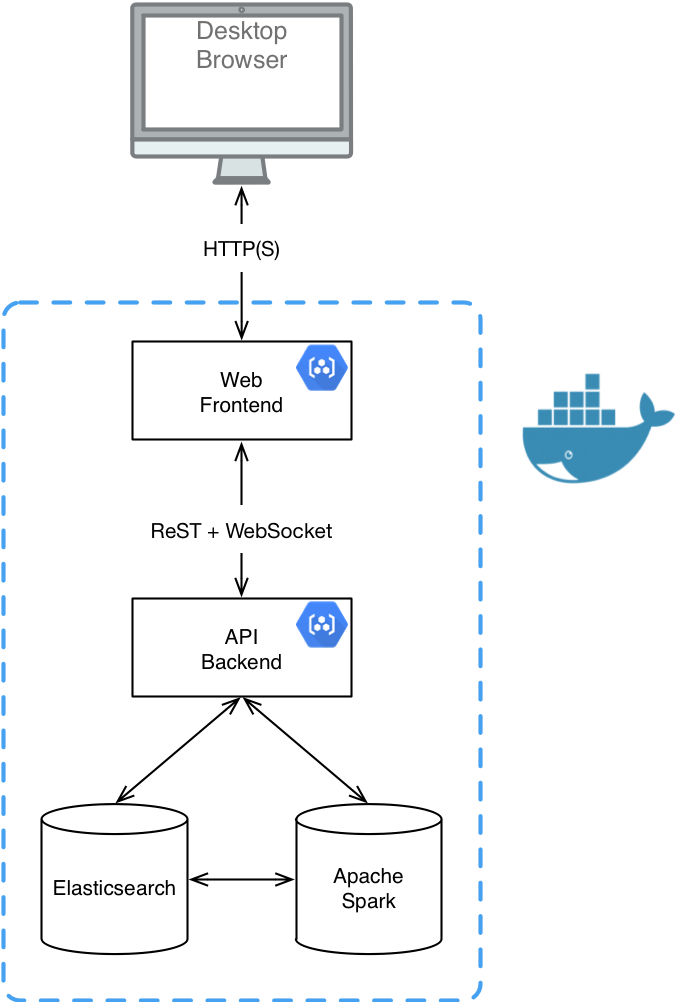
\includegraphics[width=0.75\textwidth]{figures/architecture/system-overview}
  \caption{High-level diagram of our SW architecture.}
  \label{fig:system-overview}
\end{figure}
\index{architecture}

\subsubsection{Going Live with Docker}

As mentioned above, the system is basically ``dockerized'' for container-based hosting.
I.e., the frontend as well as backend are each equipped with a fitting \emph{Dockerfile}.
Container images are based on the lightweight \emph{Alpine Linux}\footnote{\textcolor{blue}{\href{https://www.alpinelinux.org/about/}{www.alpinelinux.org/about/}}} distribution which is particularly well suited for that purpose.
In order to support an agile development process, it is easy to build and deploy the application.
More concretely, there is a \emph{Makefile} set up which allows for quick deployment of Docker images (incl. building and publishing these via private Docker repositories) to a virtual host.
The author chose in this example \emph{DigitalOcean}\footnote{\textcolor{blue}{\href{https://www.digitalocean.com/}{www.digitalocean.com}}} as hosting service provider due to the convenient \emph{\gls{dx}} it offers.

Multiple host nodes as well as multiple instances of either backend or frontend container were not relevant for the purpose of this prototype\index{prototype}.
It is generally possible to set this up and basically supported, though.
Moreover, Elasticsearch and Spark are simply being run in embedded mode within the backend component.
Again, it is generally possible to configure connection to real dedicated clusters of each.
Yet, the point of this prototype\index{prototype} was not really geared towards proving \emph{``\gls{bigdata}''} load capabilities.

On the virtual host an \emph{Nginx}\footnote{\textcolor{blue}{\href{https://nginx.org/en/}{nginx.org/en/}}} web server is configured to proxy the local containerized application servers to the public Internet.
Access to the web application is then restricted via \textsc{HTTP} basic authentication.
\textsc{HTTPS} is enabled through \emph{Let's Encrypt}\footnote{\textcolor{blue}{\href{https://letsencrypt.org/about/}{letsencrypt.org/about/}}}. \\
The interested reader may ask the author for a link with credentials.

\subsubsection{Project Structure and Setup}

In general, the system is comprised of three software projects.
One for the backend application, one for the frontend, and sort of an ``umbrella'', the master one.
The latter pulls the former ones in, via \emph{Git} submodule setup.
So, Git is used as \gls{vcs}, respectively for \gls{scm} with private \emph{Github} repositories, owned by the developer.
\gls{fs} structure of this master one also loosely resembles \emph{\glslink{cvast}{CVAST}} research group guidelines\footnote{\textcolor{blue}{\href{http://www.cvast.tuwien.ac.at/node/27}{www.cvast.tuwien.ac.at/node/27}}}.
Furthermore, it contains aforementioned Makefile for convenient builds and deployments.
The \gls{ci} tooling of choice is \emph{CircleCI}\footnote{\textcolor{blue}{\href{https://circleci.com/}{circleci.com}}}, a \gls{saas} provider with a good \gls{dx}.
Build tool of the backend project is \emph{Gradle}\footnote{\textcolor{blue}{\href{https://gradle.org/}{gradle.org}}}.
The frontend uses a combination of \emph{Yarn}\footnote{\textcolor{blue}{\href{https://yarnpkg.com/en/}{yarnpkg.com/en/}}} dependency management and \emph{Gulp}\footnote{\textcolor{blue}{\href{http://gulpjs.com/}{gulpjs.com}}} task scripts. Source code documentation is generated with \emph{Dokka}\footnote{\textcolor{blue}{\href{https://kotlinlang.org/docs/reference/kotlin-doc.html}{kotlinlang.org/docs/reference/kotlin-doc.html}}} for the backend, and \emph{ESDoc}\footnote{\textcolor{blue}{\href{https://esdoc.org/}{esdoc.org}}} for the frontend.


\subsection{Backend}

The backend mainly consists of the high-level components as laid out in Figure~\ref{fig:backend-components}.
It is basically a \emph{Spring\footnote{\textcolor{blue}{\href{projects.spring.io/spring-framework/}{projects.spring.io/spring-framework/}}} Boot\footnote{\textcolor{blue}{\href{https://projects.spring.io/spring-boot/}{projects.spring.io/spring-boot/}}}} application using \emph{Spring MVC} for its \gls{rest} controller layer.
\emph{Spring Messaging} is used for transparent WebSocket communication, and \emph{Reactor\footnote{\textcolor{blue}{\href{https://projectreactor.io/}{projectreactor.io}}} Event Bus} for reactive messaging within the outlier detection implementation.
The Elasticsearch data layer is based on \emph{Spring Data Elasticsearch\footnote{\textcolor{blue}{\href{http://projects.spring.io/spring-data-elasticsearch/}{projects.spring.io/spring-data-elasticsearch/}}}}.
Connection between Elasticsearch data storage and Apache Spark processing is done via \emph{ES-Hadoop} connector libraries\footnote{\textcolor{blue}{\href{https://www.elastic.co/guide/en/elasticsearch/hadoop/current/spark.html}{www.elastic.co/guide/en/elasticsearch/hadoop/current/spark.html}}}.

\begin{figure}[h]
  \centering
  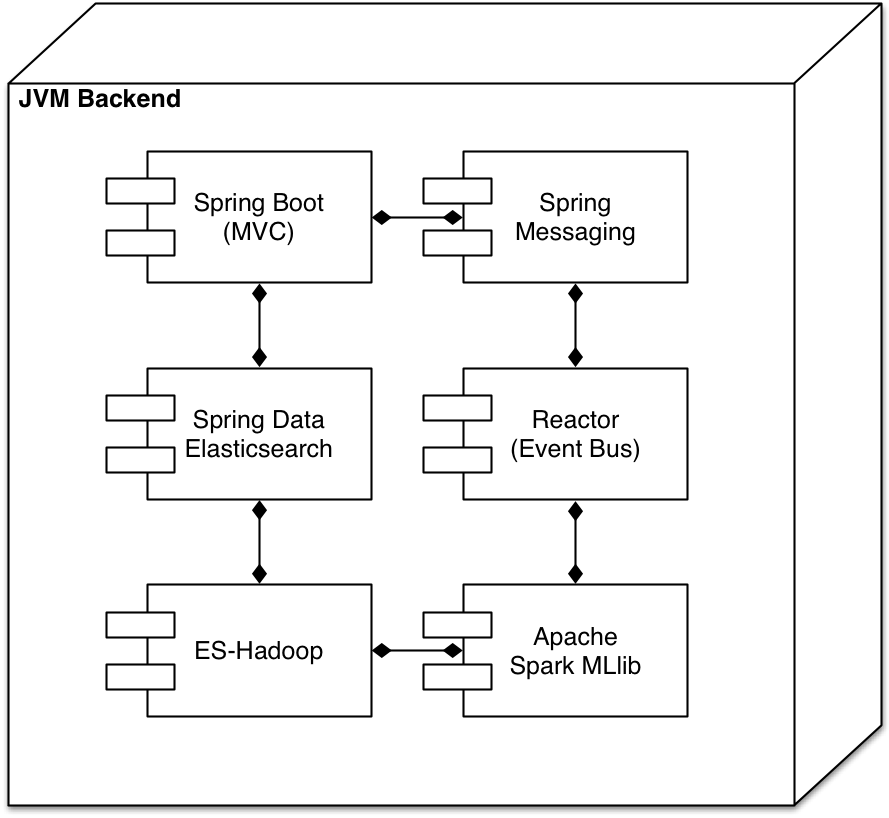
\includegraphics[width=0.75\textwidth]{figures/architecture/backend-components}
  \caption{Backend components diagram.}
  \label{fig:backend-components}
\end{figure}

Documentation of the \gls{rest} \textsc{API} is generated via \emph{Spring REST Docs\footnote{\textcolor{blue}{\href{https://projects.spring.io/spring-restdocs/}{projects.spring.io/spring-restdocs/}}}}.
This integrates nicely into the automated testing infrastructure of the project.
Thus, it can be seen as a superior solution compared to the en-vogue \emph{Swagger\footnote{\textcolor{blue}{\href{http://swagger.io/}{swagger.io}}}} in respect of it is possible to combine automated documentation generation with manually written one via
\emph{Asciidoctor\footnote{\textcolor{blue}{\href{http://asciidoctor.org/}{asciidoctor.org}}}}.

The backend project itself prefers structuring its top-level packages semantically.
E.g., there is a top-level package \emph{\textbf{importexport}} containing \emph{\textbf{dao}} (as in \emph{Data Access Object}) and \emph{\textbf{service}} sub-level packages -- not the other way round, as it would be more traditional fashion.
Unit and integration tests are present, written with state-of-the-art libraries.

Some deeper dive into the technologies employed for the backend follows.


\subsubsection{Kotlin on the JVM}

The \emph{Kotlin}\footnote{\textcolor{blue}{\href{https://kotlinlang.org/}{kotlinlang.org}}} programming language, by \emph{JetBrains}, is used on the backend.

It is a relatively young, statically typed, and concise \gls{jvm}-based language with seamless Java interoperability.
Mainly, it is adding quite some syntactic sugar, reasonably, as well as increased type inference support.
Plus, it is resolving some of Java's pain points, such as reference nullability -- a.k.a. the \emph{``billion-dollar mistake''\footnote{\textcolor{blue}{\href{http://lambda-the-ultimate.org/node/3186}{lambda-the-ultimate.org/node/3186}}}}.
Generally, it is taking a pragmatic stance and focuses on industrial software development needs.
As opposed to, e.g., Scala which can be seen as quite similar in various aspects, while being more computer science and particularly research focused, though.

Figure~\ref{fig:kotlin-sample} shows an exemplary code snippet.

\begin{figure}[h]
  \centering
  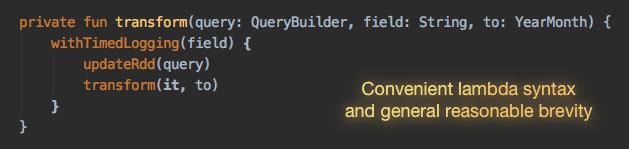
\includegraphics[width=1.0\textwidth]{figures/architecture/kotlin-sample}
  \caption{Kotlin sample demonstrating some of its useful features.}
  \label{fig:kotlin-sample}
\end{figure}

\subsubsection{Microservices with Spring Boot}

Spring Boot offers a useful approach\index{approach} to developing and running microservices. \\
It was, originally, heavily inspired by the \emph{Dropwizard}\footnote{\textcolor{blue}{\href{http://www.dropwizard.io/}{www.dropwizard.io}}} project.

The topic of building microservices itself is covered well in \cite{Newman2015}.
The basic idea here is to develop small, self-contained, and purpose-focused services with corresponding monitoring, provisioning, and orchestration capabilities.
This stands in rather stark contrast to the more traditional approach\index{approach} of building monolithic applications.
So, in general, Spring Boot provides a lot of features and abstractions with little necessary configuration out-of-the-box.
Furthermore, it integrates well with Kotlin, both sharing a pragmatic paradigm of software development philosophy.

\subsubsection{From Elasticsearch to ES-Hadoop} \label{sec:es-hadoop}

At the heart of data storage and querying, Elasticsearch is in use. \\
Spring Data Elasticsearch is providing some convenient abstractions.

As mentioned above, data processing, i.e., transformation\index{transformation} operations and outlier detection, is performed via Apache Spark and its MLlib.
Native bridging of these two popular \gls{bigdata} technologies is provided via ES-Hadoop connector libraries.
This is, basically, rooted in the fact that Apache Spark was born within the Apache Hadoop\footnote{\textcolor{blue}{\href{https://hadoop.apache.org/}{hadoop.apache.org}}} ecosystem.
Spark can be run completely independent from Hadoop infrastructure, though.
The connector libraries are officially supported and developed by \emph{Elastic\footnote{\textcolor{blue}{\href{https://www.elastic.co/}{www.elastic.co}}}}, the company behind Elasticsearch and related products.
In addition to the Scala \textsc{API}, since Spark is written in Scala, a Java \textsc{API} is available which is used in our project.

\subsubsection{Apache Spark \& MLlib}

As aforementioned, Spark is at the heart of data processing.

Its foundational construct is called \emph{\gls{rdd}}.
That is, the main concept is to provide a scalable solution for loading large datasets into memory, utilizing distributed computing.
One then can easily perform transformational\index{transformation} operations, like the common functional \emph{map} routine, on such an \gls{rdd}.
The underlying complexities are transparently hidden beneath by the abstraction.
This can be seen as fitting nicely into the philosophy of \emph{``\textbf{simple made easy}''}, as advocated by \emph{Rich Hickey}\footnote{\textcolor{blue}{\href{https://www.infoq.com/presentations/Simple-Made-Easy}{www.infoq.com/presentations/Simple-Made-Easy}}}.

Additionally, extension libraries have been built enhancing processing capabilities.
One of them is MLlib which provides convenient access to \gls{ml} algorithms.
This is used in our project for its temporal outlier detection implementation.

\subsubsection{Reactive Messaging}

Reactive programming is rather popular these days. \\
At its core stands the so-called \emph{Reactive Manifesto}\footnote{\textcolor{blue}{\href{http://www.reactivemanifesto.org/}{www.reactivemanifesto.org}}}.

It is a term for event-based programming.
That is, publish/subscribe mechanisms for message-driven communication.
Historically, it is build upon the notions from the classic \emph{Observer} pattern enhanced with functional programming techniques.
This paradigm fits especially well with the requirement of asynchronous notifications for the outlier detection component of our system. \\
Consequently, it is employed therein.

Concrete library used is Reactor and its implementation of the \emph{Event Bus} abstraction.
The former is, generally, a modern high-level take on the \emph{ReactiveX}\footnote{\textcolor{blue}{\href{http://reactivex.io/}{reactivex.io}}} approach\index{approach}.


\subsection{Frontend}

The frontend is a modern Node.js application. It is based on \emph{Este.js}\footnote{\textcolor{blue}{\href{https://github.com/este/este}{github.com/este/este}}}, a useful assembly of libraries and best practices for easily bootstrapping a universal \emph{Redux/React} project.

Its further refined stack for our project, basically, comprises of \emph{Isomorphic Fetch}\footnote{\textcolor{blue}{\href{https://github.github.io/fetch/}{github.github.io/fetch/}}} for \gls{rest} layer communication, \emph{STOMP over WebSocket}\footnote{\textcolor{blue}{\href{http://jmesnil.net/stomp-websocket/doc/}{jmesnil.net/stomp-websocket/doc/}}} with \emph{SockJS}\footnote{\textcolor{blue}{\href{http://sockjs.org/}{sockjs.org}}} for communicating with the corresponding Spring Messaging interface on the backend, a Redux\footnote{\textcolor{blue}{\href{http://redux.js.org/}{redux.js.org}}} layer containing business logic, a React\footnote{\textcolor{blue}{\href{https://facebook.github.io/react/}{facebook.github.io/react/}}} \gls{ui} as well as related URL path routing, plus \gls{ui} toolkits including \emph{D3.js}\footnote{\textcolor{blue}{\href{https://d3js.org/}{d3js.org}}} charting or common respectively extensible \gls{ui} components, and all running on an \emph{Express}\footnote{\textcolor{blue}{\href{http://expressjs.com/}{expressjs.com}}} web framework based server (see Figure~\ref{fig:frontend-components}).

\begin{figure}[h]
  \centering
  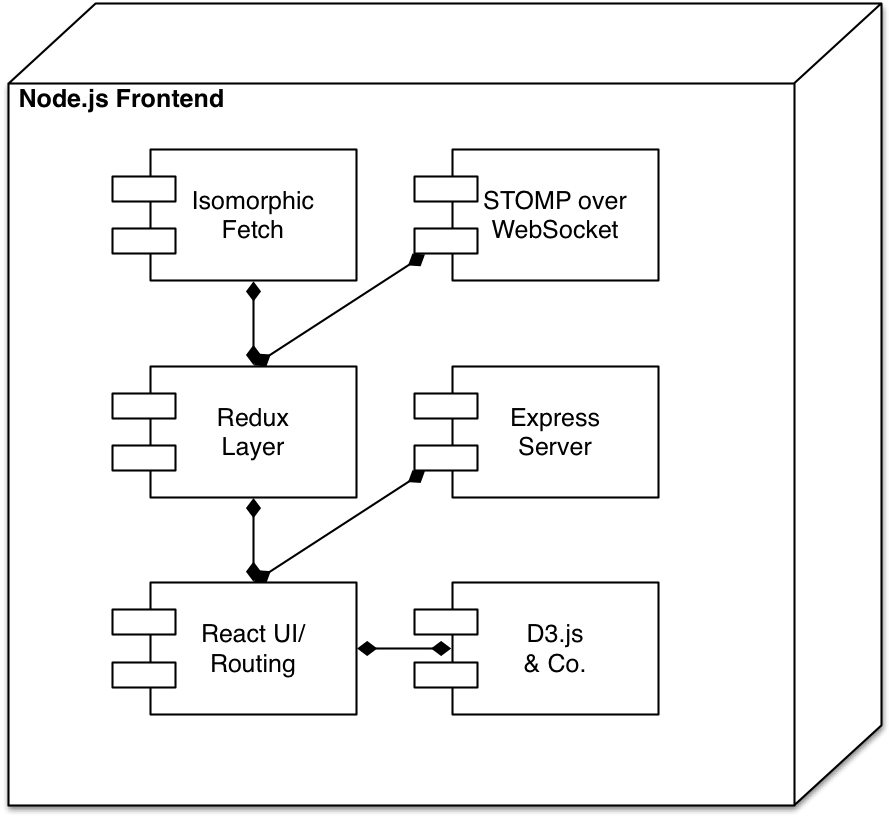
\includegraphics[width=0.75\textwidth]{figures/architecture/frontend-components}
  \caption{Frontend components diagram.}
  \label{fig:frontend-components}
\end{figure}

Project structure outlines an adapted Este scaffold. Automated testing is based on \emph{Jest}\footnote{\textcolor{blue}{\href{https://facebook.github.io/jest/}{facebook.github.io/jest/}}}.


\subsubsection{Contemporary JavaScript}

The frontend application is written in contemporary JS, that is, \emph{flow-typed\footnote{\textcolor{blue}{\href{https://flowtype.org/}{flowtype.org}}} ES6+}.

Figure~\ref{fig:react-flow-sample} is demonstrating some useful features as well as techniques when used together with Redux/React. Static type-checking is especially valuable for detecting bugs and errors early, at compile time. Compilation to common ES5 is performed via \emph{Babel}\footnote{\textcolor{blue}{\href{https://babeljs.io/}{babeljs.io}}} plus a \emph{Webpack}\footnote{\textcolor{blue}{\href{https://webpack.js.org/}{webpack.js.org}}} toolchain is in place -- minifying, optimizing, and bundling web app assets.
In addition, \emph{ESLint\footnote{\textcolor{blue}{\href{http://eslint.org/}{eslint.org}}}} helps keeping the code clean and adhering to good practices.

\subsubsection{React with Material Design}

As mentioned, the \gls{ui} is based on React.
A technology and library created at \emph{Facebook Engineering}.
It enables one to build composable \gls{ui} components in a declarative way, clearly reasoning about their state via cleanly applied \emph{\gls{soc}} pattern.
Templating is achieved with so-called \emph{JSX\footnote{\textcolor{blue}{\href{https://facebook.github.io/react/docs/introducing-jsx.html}{facebook.github.io/react/docs/introducing-jsx.html}}}}.
That is, \textsc{XML}-like syntax embedded directly in \textsc{JS} code.
Moreover, its performance is really good as partial re-rendering of to-be-updated \gls{dom} tree nodes is supported transparently.

The React programming model usually takes a bit to get accustomed to, but its benefits do pay off, especially in the long run.
Particularly, clear separation of application state and \gls{dom} is a big leap forward in this space.

General \gls{ux} of the \gls{ui} of our application is based on the \emph{Material Design\index{design}}\footnote{\textcolor{blue}{\href{https://material.io/}{material.io}}} approach\index{approach} and specification by Google.
As implementing components kit, \emph{React Toolbox}\footnote{\textcolor{blue}{\href{http://react-toolbox.com/}{react-toolbox.com}}} is used. It provides a quite comprehensive, carefully crafted set of common \gls{ui} controls and elements.
For \textsc{CSS} needs, transpiled \emph{Sass\footnote{\textcolor{blue}{\href{http://sass-lang.com/}{sass-lang.com}}}} is employed, which is pretty popular for this use case.

As mentioned before, the application is rendered client-side, as commonly expected from a \gls{spa}, yet, initially also server-side.
This isomorphic pre-rendering on the server improves the \gls{ux} by minimizing potential, irritating ``flicker'' effects on initial page load.
In particular, when loading a page with an URL which requires routing.
Additionally, it helps with \gls{seo} if applicable.
Routing is built on client \emph{HTML5 History API}\footnote{\textcolor{blue}{\href{http://diveintohtml5.info/history.html}{diveintohtml5.info/history.html}}} for clean, universal URL path layout.

\subsubsection{From Flux to Redux}

The \emph{Flux} architecture\index{architecture} was introduced by Facebook Engineering as an approach\index{approach} to better structuring \gls{spa}s.
It is based on the idea of strictly one-way data flow and binding.

This makes it much simpler to reason about an \gls{ui} system, and therefore less error-prone.
The basic concepts are shown in Figure~\ref{fig:flux-architecture} which stems from official documentation material\footnote{\textcolor{blue}{\href{https://facebook.github.io/flux/docs/in-depth-overview.html\#structure-and-data-flow}{facebook.github.io/flux/docs/in-depth-overview.html\#structure-and-data-flow}}}.
So, generally, actions are triggering system state changes and, consequently, \gls{ui} updates in a unidirectional manner.
Redux took theses concepts and further simplified them, iterating upon in its implementation.
Solutions for handling asynchronous events, as they are common in \gls{spa}s, include injecting a promise middleware into Redux as well as extending it with reactive processing via \emph{redux-observable\footnote{\textcolor{blue}{\href{https://redux-observable.js.org/}{redux-observable.js.org}}}} plus \emph{RxJS\footnote{\textcolor{blue}{\href{http://reactivex.io/rxjs/}{reactivex.io/rxjs/}}}}.
Both approaches\index{approach} are used in the prototype\index{prototype} to varying degrees with an emphasis on the former one, to get a feel for them.
A real product would most probably rather focus on one of them then.
ES6+ \emph{async/await} is helpful for coding with promises sequentially, saving one from \emph{``callback hell''}.
Immutable data structures and collections provided by \emph{Immutable.js\footnote{\textcolor{blue}{\href{https://facebook.github.io/immutable-js/}{facebook.github.io/immutable-js/}}}} are also commonly used.
Plus, \emph{Ramda\footnote{\textcolor{blue}{\href{http://ramdajs.com/}{ramdajs.com}}}} fits in well as a functional programming utilities library.
Speaking of utility libraries in our project, ones centered on temporal data processing are \emph{date-fns\footnote{\textcolor{blue}{\href{https://www.npmjs.com/package/date-fns}{www.npmjs.com/package/date-fns}}}} and \emph{js-joda\footnote{\textcolor{blue}{\href{https://js-joda.github.io/js-joda/}{js-joda.github.io/js-joda/}}}} (a \emph{java.time}-compliant \textsc{JS} port).

\begin{figure}[h]
  \centering
  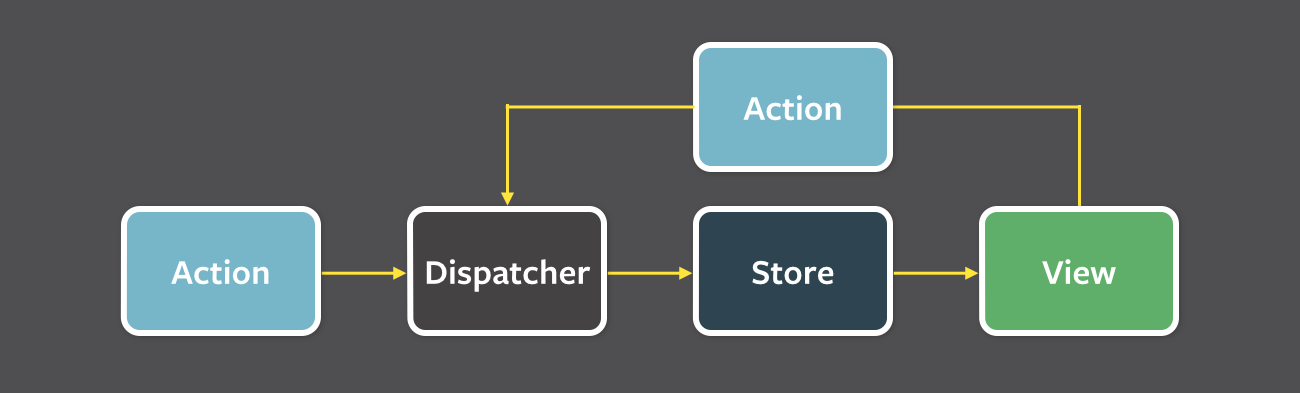
\includegraphics[width=1.0\textwidth]{figures/architecture/flux-simple}
  \caption{Simple Flux architecture diagram from Facebook Engineering.}
  \label{fig:flux-architecture}
\end{figure}
\index{architecture}

\subsubsection{Fetch API \& WebSockets}

The \emph{Fetch API} is a modern approach\index{approach} to \emph{Ajax} communication.
That is, asynchronous client/server communication of a browser application via \textsc{HTTP}.
This, traditionally, is based on usage of the so-called \emph{XMLHttpRequest} browser \textsc{JS} \textsc{API}.
The rather young Fetch \textsc{API} takes the basic concepts of async browser \gls{rest} calls and pours it into a contemporary form, conveniently usable.

\emph{WebSockets} allow for bidirectional communication.
That is, instead of solely pulling from a server, a browser client app is also able to get data pushed by the server.
It is especially useful in event-based systems, such as messaging-related ones.

\subsubsection{D3.js Charting}

\emph{D3.js} (as in \emph{Data-Driven Documents}) is a very popular \textsc{JS} library, primarily used for interactive charting.
Originally, it was developed at \emph{Stanford Vis Group} (see \cite{Bostock2011}).
It is based on \gls{svg} and surrounded by an ecosystem of components as well as extensions.

For most of the charts in our application, \emph{NVD3\footnote{\textcolor{blue}{\href{http://nvd3.org/}{nvd3.org}}}} is used.
It is a useful repository of various ready-to-use charts, all conveniently customizable.
Plus, they are nicely crafted with appealing default look \& feel, supporting decent animations.
Figure~\ref{fig:nvd3-gallery} shows an overview gallery from their documenting website.
Our calendar heatmap visualization component is based on \emph{cal-heatmap\footnote{\textcolor{blue}{\href{http://cal-heatmap.com/v2/}{cal-heatmap.com/v2/}}}}.
It is a widely used implementation with a multitude of customization and tweaking options.
Integration of D3 with React works, all in all, relatively straightforward. Yet, some resorting to direct \gls{dom} manipulation and event handling is required, unfortunately, due to legacy reasons inflicted by the former.

\begin{figure}[h]
  \centering
  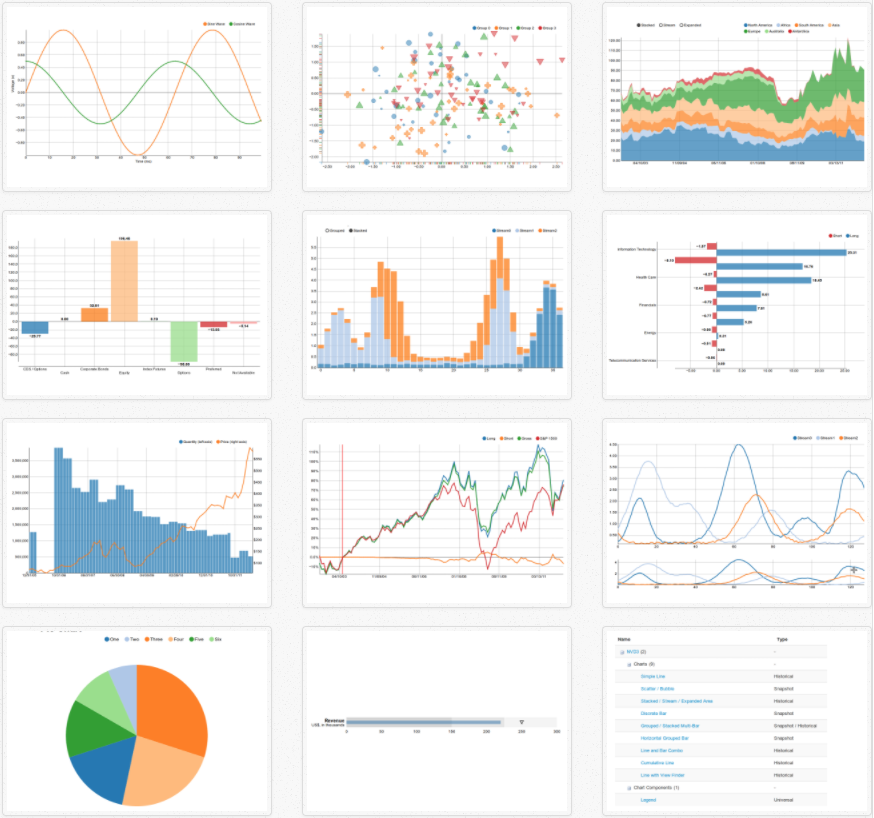
\includegraphics[width=0.825\textwidth]{figures/architecture/nvd3-gallery}
  \caption{A screenshot of an NVD3 charts gallery, as presented on nvd3.org.}
  \label{fig:nvd3-gallery}
\end{figure}

\begin{figure}[h]
  \centering
  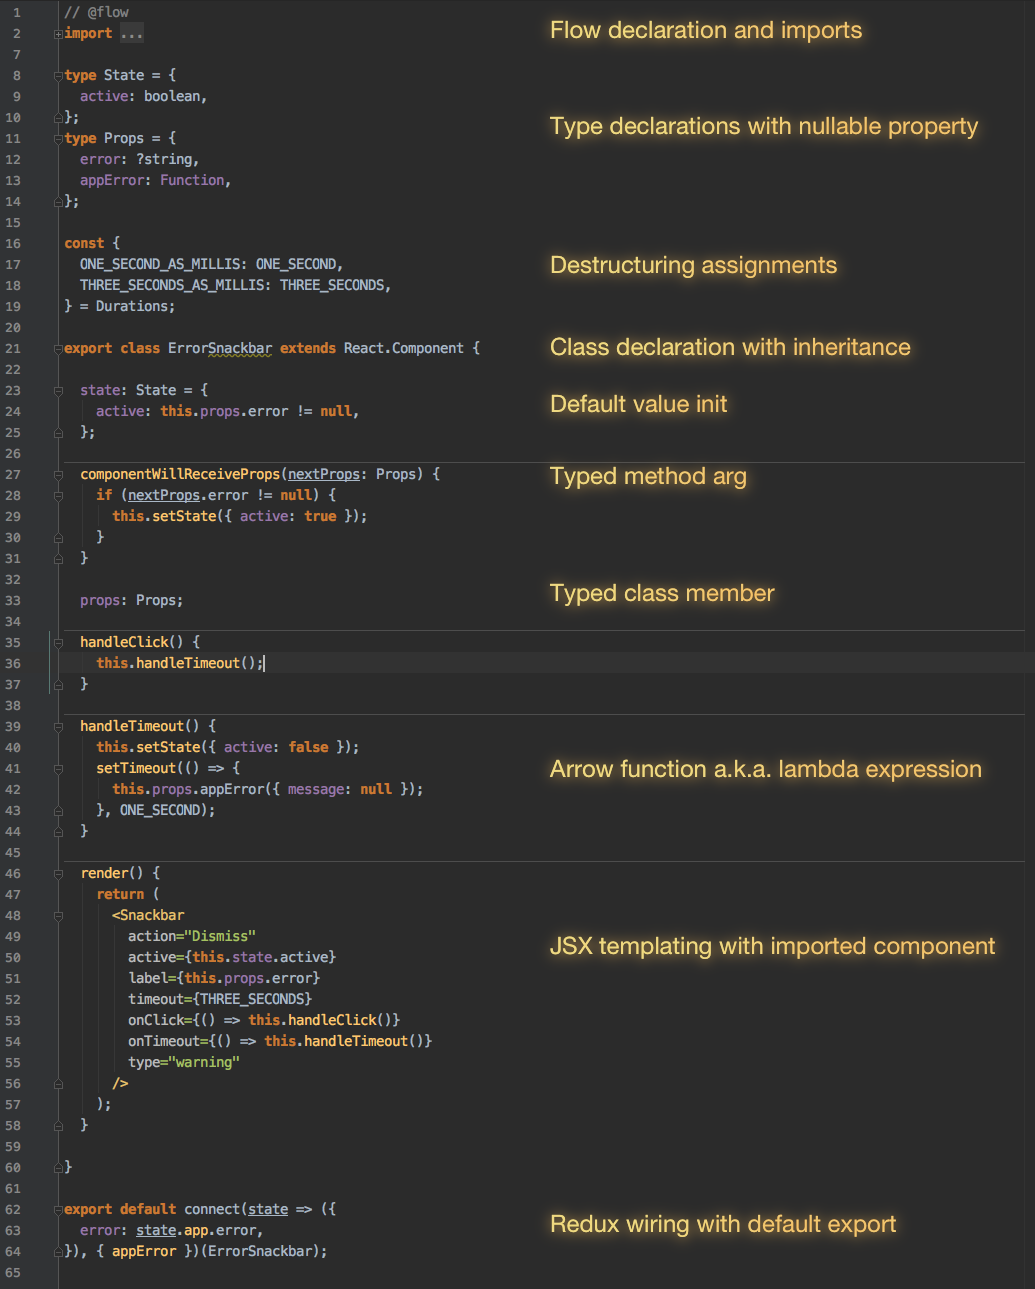
\includegraphics[width=1.05\textwidth]{figures/architecture/react-flow-sample}
  \caption{Flow-typed ES6+ Redux/React \gls{ui} component showing some useful features.}
  \label{fig:react-flow-sample}
\end{figure}



%%%%%%%%%%%%%%%%%%%%%%%%%%%%%%%%%%%%%%%%%
\chapter{Information Retrieval Background}
\label{ch:appendix-b}
%%%%%%%%%%%%%%%%%%%%%%%%%%%%%%%%%%%%%%%%%

In this appendix some \gls{ir} background is presented, as core data storage and querying of our prototype\index{prototype} is based on.

\subsubsection{TF-IDF \& Apache Lucene}

The equations~\ref{eq:ir-tf-1} to~\ref{eq:ir-tf-idf} lay out some of the most fundamental concepts behind \gls{ir}.

\begin{equation}
\text{tf}(t, d) = f_{t,d}
\label{eq:ir-tf-1}
\end{equation}

\begin{equation}
f_{t,d} =
\begin{cases}
  1 \quad \text{if } t \text{ occurs in } d \\
  0 \quad \text{otherwise} \\
\end{cases}
\label{eq:ir-tf-2}
\end{equation}

\begin{equation}
\text{idf}(t, D) = \log\frac{N}{|\{d \in D : t \in d\}|}
\label{eq:ir-idf}
\end{equation}

\begin{equation}
\text{tf-idf}(t, d, D) = \text{tf}(t, d) \times \text{idf}(t, D)
\label{eq:ir-tf-idf}
\end{equation}

It is \emph{\gls{tf-idf}}\footnote{\textcolor{blue}{\href{https://en.wikipedia.org/wiki/Tf-idf}{en.wikipedia.org/wiki/Tf-idf}}}.
Basically, this is an effective as well as efficient way to score term query search hits based on term occurrences in a corpus of documents.
The illustrated formula set uses a simple boolean frequency.

A popular and high-quality search engine implementation in Java is \emph{Apache Lucene\footnote{\textcolor{blue}{\href{https://lucene.apache.org/}{lucene.apache.org}}}}.
It is also the foundation on which Elasticsearch is built upon~\cite{Gormley2015}.



%%%%%%%%%%%%%%%%%%%%%%%%%%%%%%%%%%%%%%%%%
\chapter{Supported Date/Time Formats}
\label{ch:appendix-c}
%%%%%%%%%%%%%%%%%%%%%%%%%%%%%%%%%%%%%%%%%

Our data model, generally, supports following date/time formats\footnote{Cf. \textcolor{blue}{\href{https://docs.oracle.com/javase/8/docs/api/java/time/format/DateTimeFormatter.html}{docs.oracle.com/javase/8/docs/api/java/time/format/DateTimeFormatter.html}}} for automatic parsing:

\begin{itemize}
  \item \emph{ISO\_ORDINAL\_DATE}
  \item \emph{BASIC\_ISO\_DATE}
  \item \emph{ISO\_DATE}
  \item \emph{ISO\_DATE\_TIME}
  \item \emph{ISO\_ZONED\_DATE\_TIME}
  \item \emph{yyyy/MM/dd}
  \item \emph{yyyy/MM/dd HH:mm[:ss[.SSS]]}
  \item \emph{MM/dd/yyyy}
  \item \emph{MM/dd/yyyy HH:mm[:ss[.SSS]]}
  \item \emph{dd/MM/yyyy}
  \item \emph{dd/MM/yyyy HH:mm[:ss[.SSS]]}
  \item \emph{dd.MM.yyyy}
  \item \emph{dd.MM.yyyy HH:mm[:ss[.SSS]]}
  \item \emph{EPOCH\_MILLIS}
\end{itemize}



\backmatter

% Use an optional list of figures.
\listoffigures % Starred version, i.e., \listoffigures*, removes the toc entry.

% Use an optional list of tables.
\cleardoublepage % Start list of tables on the next empty right hand page.
\listoftables % Starred version, i.e., \listoftables*, removes the toc entry.

% Use an optional list of alogrithms.
\listofalgorithms
\addcontentsline{toc}{chapter}{List of Algorithms}

% Add an index.
\printindex

% Add a glossary.
\printglossaries

% Add a bibliography.
\bibliographystyle{alpha}
\bibliography{references}

\end{document}
